% !TEX encoding = IsoLatin

%%%%%%% La riga soprastante serve per configurare gli editor TeXShop, TeXWorks
%%%%%%% e TeXstudio per gestire questo file con la codifica IsoLatin o Latin 1
%%%%%%% o ISO 8859-1. Se si vuole usare un'altra codifica si veda sotto.
%%%%%%%
\documentclass[12pt,classica, italian]{toptesi}

%%%%%%%%%%%%%%%%%%%%%%%%%%%%%%%%%%%%%%%%%%%%%%%%%%%%%%%%%%%%%%%

% INCLUSIONE PACCHETTI
\usepackage[utf8]{inputenc} %utf8
\usepackage[italian]{babel}
\usepackage[T1]{fontenc}
\usepackage{blindtext}
\usepackage{graphicx,wrapfig}
\usepackage{booktabs}
\usepackage{lmodern}
\usepackage{varioref}
\usepackage{url}
\usepackage{array}
\usepackage{paralist}{\obeyspaces\global\let =\space}
\usepackage{verbatim} 
\usepackage{subfig}
\usepackage{tabularx}
\usepackage{amsmath}
\usepackage{amsfonts}
\usepackage{float}
\usepackage{amssymb}
\usepackage{multicol}
\usepackage{multirow}
\usepackage{listings}
\usepackage[pass]{geometry}
\usepackage[figuresright]{rotating}
\usepackage{algorithm}
\usepackage{algorithmic}
\usepackage{amsmath}
\usepackage[babel]{csquotes}
\usepackage{hyperref}


\usepackage[backend=bibtex]{biblatex}

%%%%%%%%%%%%%%%%%%%%%%%%%%%%%%%%%%%%%%%%%%%%%%%%%%%%%%%%%%%%%%%

\def\myfig#1{Figura~#1\xspace}

%%%%%%%%%%%%%%%%%%%%%%%%%%%%%%%%%%%%%%%%%%%%%%%%%%%%%%%%%%%%%%%

% CONFIGURAZIONE LINK E RIFERIMENTI
\hypersetup{%
    pdfpagemode={UseOutlines},
    bookmarksopen,
    pdfstartview={FitH},
    colorlinks,
    linkcolor={black}, %COLORE DEI RIFERIMENTI AL TESTO
    citecolor={blue}, %COLORE DEI RIFERIMENTI ALLE CITAZIONI
    urlcolor={blue} %COLORI DEGLI URL
}

%%%%%%%%%%%%%%%%%%%%%%%%%%%%%%%%%%%%%%%%%%%%%%%%%%%%%%%%%%%%%%%

% CONFIGURAZIONE LISTATI/CODICE - CANCELLARE SE NON NECESSARIO
% PYTHON - BIANCO E NERO
\lstset{%
	captionpos=b,
	language=Python,
	basicstyle =\small\ttfamily,
	keywordstyle=\color{black}\bfseries,
	breaklines=true,
	breakatwhitespace=true,
	frame=lines,
	numbers=left,
	numberstyle=\footnotesize,
}

%%%%%%%%%%%%%%%%%%%%%%%%%%%%%%%%%%%%%%%%%%%%%%%%%%%%%%%%%%%%%%%

% FRENCHSPACING ABILITATO - CANCELLARE PER SPAZIATURA ALL'INGLESE
%\frenchspacing

%%%%%%%%%%%%%%%%%%%%%%%%%%%%%%%%%%%%%%%%%%%%%%%%%%%%%%%%%%%%%%%

%DEFINIZIONE SEZIONI IN NUMERAZIONE ROMANA
%ELENCO DEI LISTATI/CODICI
\makeatletter
\newcommand\listofcodes{%
 \iffrontmatter\else\frontmattertrue\fi
 \if@openright\cleardoublepage\else\clearpage\fi
 % change the meaning of \chapter in a group
 \begingroup\def\chapter##1{\@schapter}
 \phantomsection % for the hyperlink
 \lstlistoflistings 
 \endgroup
} 
\makeatother

%%%%%%%%%%%%%%%%%%%%%%%%%%%%%%%%%%%%%%%%%%%%%%%%%%%%%%%%%%%%%%%

% INFORMAZIONI PDF - PERSONALIZZARE
\pdfinfo{%
  /Title    (Design e sviluppo di un Serious Game in ambito museale)
  /Author   (Corrado Raffaelli)
  /Author   (Dario Randazzo)
}


% LISTA DEI CAPITOLI DA INCLUDERE - PERSONALIZZARE
\includeonly{%
	chapters/Introduzione,
	chapters/ContestoDiRiferimento,
	chapters/StatoDellArte,
	chapters/GameDesign,
	chapters/GameDevelopment,
	chapters/Risultati
	%	appendixes/appendix,
}

% FILE DI BIBLIOGRAFIA
\bibliography{bibliography, bibliographyDario} 
%\bibliography{bibliographyDario} 

%%%%%%%%%%%%%%%%%%%%%%%%%%%%%%%%%%%%%%%%%%%%%%%%%%%%%%%%%%%%%%%
\begin{document}
% FRONTESPIZIO - PERSONALIZZARE
% ELIMINATE LE VOCI CHE NON VI SERVONO

% UNIVERSITA - NOME
\ateneo{Politecnico di Torino}

% FACOLTA - DICITURA
\FacoltaDi{III Facoltà di }
% FACOLTA - NOME
\facolta{Ingegneria}

% CORSO DI LAUREA - DICITURA (MANTENERE LO SPAZIO)
\CorsoDiLaureaIn{Corso di Laurea in }
% CORSO DI LAUREA - NOME
\corsodilaurea{Ingegneria Informatica}

% TIPOLOGIA TESI
\TesiDiLaurea{Tesi di Laurea Magistrale}

% TITOLO
\titolo{Design e sviluppo di un Serious Game in ambito museale}

% SOTTOTITOLO
%\sottotitolo{How to write meaningful titles}

% RELATORE/I - DICITURA
\AdvisorName{Relatore}
% RELATORE - PROF. NOME E COGNOME
\relatore{prof.\ Andrea Bottino}
% RELATORE AGGIUNTIVO - PROF NOME E COGNOME
% SE SI HA SOLO UN RELATORE ELIMINARE E CAMBIARE Advisors in Advisor
%\secondorelatore{prof.\ Neo Cortex}

% TUTORE AZIENDALE - TITOLO NOME E COGNOME
%\tutoreaziendale{Ing. Pug Dog}
% TUTORE AZIENDALE - DICITURA//AZIENDA
%\NomeTutoreAziendale{Company tutors\\FeelGood Inc}

% CANDIDATO - DICITURA (MANTENERE I DUE PUNTI)
\CandidateName{Candidati:}
% SECONDO CANDIDATO - ELIMINARE O DECOMMENTARE
%secondocandidato{Bombo de Bombis}

% CANDIDATO - NOME E COGNOME
\candidato{Corrado Raffaelli}
\secondocandidato{Dario Randazzo}

% LOGO UNIVERSITA
\logosede{images/logo_polito}

% DATA - MESE ANNO
\sedutadilaurea{Ottobre 2015}

%%%%%%%%%%%%%%%%%%%%%%%%%%%%%%%%%%%%%%%%%%%%%%%%%%%%%%%%%%%%%%%




%%%%%%%%%%%%%%%%%%%%%%%%%%%%%%%%%%%%%%%%%%%%%%%%%%%%%%%%%%%%%%%

% INIZIO DOCUMENTO
%\begin{document}
%\english

\frontespizio

%\paginavuota




%%%%%%%%%%%%%%%%%%%%%%%%%%%%%%%%%%%%%%%%%%%%%%%%%%%%%%%%%%%%%%%

%INTERLINEA - DEFAULT 1 - NON ESAGERATE, NON SUPERATE MAI 1.3 ;)
\interlinea{1.3}

%%%%%%%%%%%%%%%%%%%%%%%%%%%%%%%%%%%%%%%%%%%%%%%%%%%%%%%%%%%%%%%

\frontmatter
\begin{comment}
% DEDICA - PERSONALIZZARE
% VSPACE - PROPORZIONE USATA PER CENTRATURA VERTICALE DEL TESTO
% FLUSHRIGHT - ALLINEAMENTO ORIZZONTALE A DESTRA
\vspace*{\stretch{1}}
\begin{flushright}
\noindent
grazie a tutti
\end{flushright}
\vspace*{\stretch{6}}
\cleardoublepage
\end{comment}
% CITAZIONE - PERSONALIZZARE
% VSPACE - PROPORZIONE USATA PER CENTRATURA VERTICALE DEL TESTO
% FLUSHRIGHT - ALLINEAMENTO ORIZZONTALE A DESTRA
\vspace*{\stretch{1}}
\begin{flushright}
\noindent


\textit{Games shouldn't only be fun.} 
	
\textit{They should teach or spark an interest in other things.}

Hideo Kojima
\end{flushright}
\vspace*{\stretch{6}}
\cleardoublepage

%

%%%%%%%%%%%%%%%%%%%%%%%%%%%%%%%%%%%%%%%%%%%%%%%%%%%%%%%%%%%%%%%
% added by Matteo, used to modify the depth of 
% numbering the subsections
\setcounter{secnumdepth}{4}
% listing the subsections in the table of contents
\setcounter{tocdepth}{3}
\newcommand{\servecitazione}[1]{\textcolor{blue}{\textbf{citare qualcosa : #1}}}
\newcommand{\needsrevision}[1] {\textcolor{green}{\textbf{needs revision: #1}}}
\newcommand{\matteo}[1] {\textcolor{green}{\textbf{Matteo: #1}}}
\newcommand{\matteodubbio}[1] {\textcolor{red}{\textbf{questa Matteo non l'ha capita "#1"}}}
\newcommand{\fabiodubbio}[1] {\textcolor{red}{\textbf{Fabio non riesce a capire perche' ha scritto queste vaccate "#1"}}}
\newcommand{\imageneeded}[1] {\textcolor{blue}{\textbf{Image is needed "#1"}}}
\newcommand{\fabio}[1] {\textcolor{green}{\textbf{Fabio: #1}}}

\newcommand{\manclass}[1]{\emph {#1} }

%%%%%%%%%%%%%%%%%%%%%%%%%%%%%%%%%%%%%%%%%%%%%%%%%%%%%%%%%%%%%%%

% RINGRAZIAMENTI - PERSONALIZZARE
\ringraziamenti
There are a lot of people who deserve to be named. First of all, all the guys in ``Lab 9'', especially Ivano Cerrato and Alex Palesandro, each of them has helped me in these eight months of thesis, and from whom I learned a lot. Thank you to Matteo Tiengo, for staying up late at night with me in the laboratory, and thank you to the annoying alarm of ``Politecnico di Torino'', for reminding us the ending of the canonical hours. Thank you to my university supervisor Fulvio Risso for all the precious advice and continuous support. 

Thank you to Andrea and Corrado, without whom I would never have come to Torino.
Thank you to my cousin Catia, that supported me in difficult moments in a city far from home. 
Thank you to my parents, who gave me this fantastic opportunity.

I would thank all my friends in my hometown Cupra Marittima, that every time I come home they make me feel as if I never left. 
I would also thank all people I met during the years in Torino.


%%%%%%%%%%%%%%%%%%%%%%%%%%%%%%%%%%%%%%%%%%%%%%%%%%%%%%%%%%%%%%%
\begin{comment}
% ABSTRACT - PERSONALIZZARE
\sommario
Abstract, pleased to meet you. Ah, it's not funny anymore.
\end{comment}
%%%%%%%%%%%%%%%%%%%%%%%%%%%%%%%%%%%%%%%%%%%%%%%%%%%%%%%%%%%%%%%

% INDICI - ELIMINARE GLI INDICI NON NECESSARI

% INDICE GENERALE
\tableofcontents

% INDICE DELLE FIGURE
\listoffigures

% INDICE DELLE TABELLE
\listoftables

% INDICE DEI CODICI
%\listofcodes

%\paginavuota

%%%%%%%%%%%%%%%%%%%%%%%%%%%%%%%%%%%%%%%%%%%%%%%%%%%%%%%%%%%%%%%

\mainmatter

% INCLUSIONE FILE CAPITOLI - PERSONALIZZARE - TENERE COERENTE CON LISTA IN ALTO
\chapter{Introduzione}
\label{chap:intro}

Il lavoro di Tesi si pone come obiettivo il design e lo sviluppo di un prototipo di videogioco, della tipologia \textit{Serious Game}, che possa aiutare l’avvicinamento dei ragazzi in età adolescenziale al contesto museale.

È stato svolto presso l’azienda \textit{e-Mentor}, nata a Torino nel 2004 per iniziativa dell’Ing. Manuela Martini, caratterizzata negli anni per lo sviluppo di soluzioni innovative per istituzioni, organizzazioni e aziende in ambito \textit{e-learning}, \textit{web \& mobile design}, \textit{edutainment} e \textit{software engineering} (Capitolo~\ref{sec:azienda}).

Il Museo del Cinema di Torino, da tempo pone l’attenzione al problema della poca affluenza di ragazzi in età adolescenziale, cercando soluzioni originali che possano invertire questa tendenza. Un'analisi più approfondita è fornita nel Capitolo~\ref{sec:situazione_museale}.

La collaborazione tra e-Mentor e Museo del Cinema nasce, nel 2013, per provare a porre rimedio a questo problema.
Tra le prime soluzioni proposte c’è quella di sviluppare un videogioco che avvicini i ragazzi a tematiche trattate all’interno del Museo. In seguito a mesi di lavoro e riunioni tra esperti dell’ambito \textit{learning}, artistico e del videogame, viene prodotto un documento di Design, che contiene idee di meccaniche, ambientazioni e scenari di gioco. Le tematiche che si è deciso di trattare sono quelle del \textit{pre-Cinema}, caratterizzato da tecnologie, oggettistica e curiosità per lo più ignoti al pubblico.
Il documento di Design viene presentato al bando \textit{Creative Europe, MEDIA Sub-programme, Support for Concept and Project Development of Video Games}, del Marzo 2014 (Capitolo~\ref{sec:azienda_precedente}).
L’idea di Design viene accolta positivamente, ma la domanda viene scartata perché il progetto viene considerato poco definito, con alcuni elementi di gameplay non adatti ad essere finanziati e quindi lanciati sul mercato.

Il progetto, ormai denominato \textit{The Magic Lantern}, è stato momentaneamente accantonato, fino al nostro inserimento nel Dicembre del 2014.
Il nostro lavoro è nato con lo scopo di creare un prototipo di gioco funzionante, con cui poter testare idee di design, meccaniche e tecniche di fruizione di contenutistica efficaci.
Le riunioni preliminari si sono quindi focalizzate nel formare un team di lavoro, oltre che stabilire una timeline per organizzare le varie fasi dello sviluppo, approfondibili nel Capitolo~\ref{sec:dev_fasi_sviluppo}.
L’attività svolta può quindi essere divisa in due grandi momenti:

\begin{itemize}
	\item \textbf{Pre-Production}. Durante la quale ci siamo occupati di una revisione del concept iniziale, aggiornandolo e arricchendolo di elementi interessanti, oltre che della prototipazione delle varie soluzioni proposte così da poterle validare.
	\item \textbf{Production}. Caratterizzata da un raffinamento del design fatto nella fase di pre-production, sviluppo del prototipo, accompagnato dall’art ed audio production e quindi la nascita della First Playable.
\end{itemize}

Per la fase di sviluppo ci siamo avvalsi di \textit{Unity3D}, motore di gioco gratuito per la creazione di videogiochi e contenuti interattivi e di \textit{GIT}, come sistema di \textit{versioning}, per la sincronizzazione del lavoro tra i membri del team (Capitolo~\ref{sec:dev_strumenti}).

Il design del gioco è quindi iniziato con l’idea di sviluppare un prodotto adatto ad un pubblico della fascia di età compresa tra i 12 ed i 16 anni. Le tematiche trattate e le metafore di gioco sarebbero quindi dovute essere coerenti con ragazzi in periodo adolescenziale.
I prodotti sviluppati, in ambito museale, con finalità di intrattenimento, possono porsi in tre differenti momenti in relazione alla visita al museo, approfonditi nel Paragrafo~\ref{sec:piattaforma_di_riferimento}, che vengono definiti come:

\begin{itemize}
	\item \textbf{Pre-Visita}.
	\item \textbf{Visita}.
	\item \textbf{Post-Visita}.
\end{itemize}

Abbiamo quindi inizialmente scartato l’idea di sviluppare un prodotto finalizzato al momento della Visita, perché non coerente con l’obiettivo primario di avvicinamento dei giovani della fascia di età di riferimento. Ci si è quindi focalizzati alla produzione di una soluzione adatta sia ai momenti precedenti che successivi all’ingresso al museo. Questa scelta ha permesso di ideare un prodotto con la funzione di incuriosire i ragazzi nei confronti di tematiche a loro abbastanza sconosciute, così da indurli ad approfondire tali argomenti attraverso una visita al Museo, oltre che adatto a mantenere contatto con i temi eventualmente già apprezzati durante una precedente visita.

Risulta importante specificare come, anche su richiesta del Museo del Cinema, le tematiche non sarebbero dovute essere affrontate in maniera didascalica e didattica, per non rischiare di annoiare o frustrare il giocatore, ma anzi, lo scopo sarebbe dovuto essere esclusivamente quello di incuriosire nei confronti di temi non molto noti.

In seguito all’analisi del contesto ci siamo quindi dedicati al vero design di gioco, scegliendo in primo luogo le principali tipologie di meccaniche da utilizzare, argomento trattato nel Capitolo~\ref{sec:meccaniche}. Abbiamo valutato la possibilità di usare elementi tipici di videogiochi \textit{platform}, molto intuitivi e familiari, così da facilitare l’immediatezza del prodotto (Capitolo~\ref{platform}). Il gioco è inoltre basato su una importante componente \textit{puzzle}, che ci ha permesso di utilizzare in maniera originale alcune tecnologie del pre-Cinema come metafore di gioco (Capitolo~\ref{sec:meccaniche_serious}).
Secondo quello che si è stabilito durante il design di gioco, questo dovrebbe essere caratterizzato, nel prodotto finito, da ambientazioni caratteristiche, che richiamino gli spettacoli dell’epoca. Poiché, come già specificato, lo scopo del progetto è la creazione di un prototipo atto a verificare l’efficacia di alcune scelte e tecniche usate, la componente artistica si è limitata a quegli elementi che avrebbero potuto influire sulla comprensibilità del \textit{gameplay}.

Per quando riguarda la componente di gioco \textit{Serious}, si è deciso di fare uso di una meccanica principale, dominante sulle altre, quella della Lanterna Magica, da cui il progetto prende il nome. La Lanterna è considerata l’antenato del proiettore. Generava proiezioni a colori ed in movimento, con un effetto così stupefacente da far credere, al pubblico del ‘600, che le immagini prodotte fossero reali. La meccanica sviluppata è quindi quella di far utilizzare uno strumento capace di cambiare lo scenario con le proiezioni, sulla base dei vetrini disponibili. Si può fare riferimento al Capitolo~\ref{sec:precinema} per maggiori informazioni sulle tecnologie del pre-cinema.

Oltre alla meccanica della Lanterna Magica, ne sono state aggiunte altre che rappresentano metafore delle tecnologie del pre-Cinema. Tra queste ci sono le lenti, utilzzate nel gioco per ingrandire e rimpicciolire il personaggio e la Camera Oscura che, al momento dell’interazione, ruota la camera di 180 gradi, così da dare la sensazione che il mondo sia invertito. L’utilizzo di tali meccaniche è stato limitato a piccole porzioni di gioco, in quanto fornire un numero eccessivo di possibilità al giocatore, rischia di confonderlo e sviare l’attenzione verso obiettivi non previsti.

Oltre alle meccaniche di gioco elencate, sono stati inseriti alcuni elementi estetici coerenti con il pre-Cinema, come Lanterne Magiche che generano nemici, o proiezioni caratteristiche.

Per quanto riguarda la fruizione di contenuti, questa è permessa attraverso la lettura di schede informative, ottenibili dal raccoglimento di oggetti nello scenario, dal dialogo con personaggi non giocabili o con il semplice proseguire con l’avventura. L'analisi delle schede informative è trattata nel Capitolo~\ref{sec:schede_informative}.
I personaggi non giocabili permettono anche di ottenere oggetti collezionabili tramite dei semplici questionari. Questo permette un maggiore interessamento dei giocatori alle schede informative, soprattutto di quelli più portati al completamento dell’avventura in ogni sua componente.

La validazione dello soluzioni sviluppate è avvenuta tramite due sessioni di testing, la prima nel Luglio 2015, presso un oratorio salesiano, la seconda, nell' Ottobre 2015, presso l’ITIS Majorana di Grugliasco (riferimento).
In seguito all’analisi dei risultati ottenuti dal primo test, abbiamo notato un generale apprezzamento del gameplay e delle meccaniche di gioco, ma un basso interesse verso la tematica del pre-Cinema, sottolineato sia dalla bassa percentuale di apertura delle schede informative, che dalle risposte fornite al questionario anonimo che abbiamo ritenuto utile far compilare a fine sessione (riferimento).
Abbiamo quindi studiato ed implementato delle soluzioni per risolvere questi problemi, tra cui i già citati personaggi non giocabili e le sezioni con lenti e camera oscura. Oltre questo, abbiamo dato la possibilità di osservare contenuti delle schede informative nelle schermate di caricamento e in alcune sezioni particolari dello scenario di gioco (Capitolo~\ref{sec:contestualizzazione_elementi}).
I risultati ottenuti dal secondo test hanno confermato che le soluzioni adottate sono state efficaci. I tester infatti, hanno mostrato un discreto interesse nell’approfondire argomenti presentati tramite meccaniche o solo dal punto di vista estetico, tramite l’apertura e la lettura delle schede informative.

Ora che il prototipo e le soluzioni proposte sono state validate, il passaggio successivo sarà quello di una nuova sessione di Design che porti alla definizione del prodotto finale che dovrà raggiungere il mercato, mirata anche ad una ristrutturazione dell’idea, sulla base di un’attenta analisi per ingegnerizzazione del prodotto.


\chapter {Contesto di riferimento}
\label{chap:contesto}

\section{Tematiche e contesto museale}
\label{sec:contesto_museale}

\subsection{Pre-Cinema}
\label{sec:precinema}

Il Cinema è un media di comunicazione di grandissimo impatto. È da lungo tempo un’arte che attira un grande numero di appassionati e di esperti. È soggetto di studi, di analisi e di approfondimenti.
Purtroppo però, le ricerche che hanno portato alla nascita del Cinema sono per lo più sconosciute al pubblico. 
Con il termine \textit{pre-cinema} si fa quindi riferimento a tutti quegli studi e tecnologie antecedenti la nascita del Cinema, datata 28 Dicembre 1895, con la prima proiezione ufficiale dei fratelli Lumière.

L’idea di sfruttare la tematica del pre-cinema per il progetto sviluppato nasce quindi dalla convinzione di poter generare curiosità riguardo una tematica non molto nota, ma verso cui esiste una base di conoscenza radicata.
Secondo Wikipedia \cite{precinema_wikipedia} “col termine pre-cinema si intendono tutti quegli esperimenti e intrattenimenti legati alla proiezione di immagini ed al movimento illusorio databili dall’antichità fino alla prima proiezione pubblica di cinematografo, organizzata dai fratelli Lumière il 28 Dicembre 1895”. 

Si parla quindi di proiezioni e dispositivi ottici, che nascono come semplici studi, per poi essere portati ad essere spettacoli per vasti pubblici. Gli spettatori erano affascinati dalle immagini e dalle esperienze che stavano vivendo, da arrivare a considerare magici gli strumenti e le tecnologie che le producevano.
Di seguito vengono analizzate alcune tecnologie e spettacoli che si sono rivelati interessanti per lo sviluppo del nostro prototipo, molte informazioni riportate sono state tratte dal libro “Quando il cinema non c’era” di Donata Pesenti Campagnoni \cite{quando_il_cinema_non_cera}:

\begin{itemize}
	\item \textbf{Camera Oscura.}
	\label{contesto_camera_oscura}
	È un dispositivo ottico basato su una scatola con un piccolo foro su di una faccia ed un piano di proiezione dell’immagine sulla faccia opposta. La luce, entrando dal foro, proietta sulla faccia opposta della scatola l’immagine capovolta di quello che si trova di fronte al foro.
	
	Il fenomeno empirico della Camera Oscura è in realtà noto sin dall’antichità, riferimenti si possono trovare già in autori come Euclide e Aristotele.
	Per molto tempo è utilizzata per osservare eclissi solari, e solo dal ‘400 in poi se ne sottolinea il potere di riprodurre immagini di ciò che ci circonda. “Leonardo da Vinci mette in luce l’analogia tra camera oscura ed occhio umano […] e da lì in poi il processo fisiologico della visione verrà spiegato sempre più spesso facendo ricorso a questo particolare fenomeno empirico a tal punto da farlo diventare, nel corso del Seicento e del Settecento, il modello più utilizzato nel campo dell’ottica fisica, la metafora per definizione dell’occhio e del suo funzionamento.
	
	\begin{figure}%[h]
		\centering
		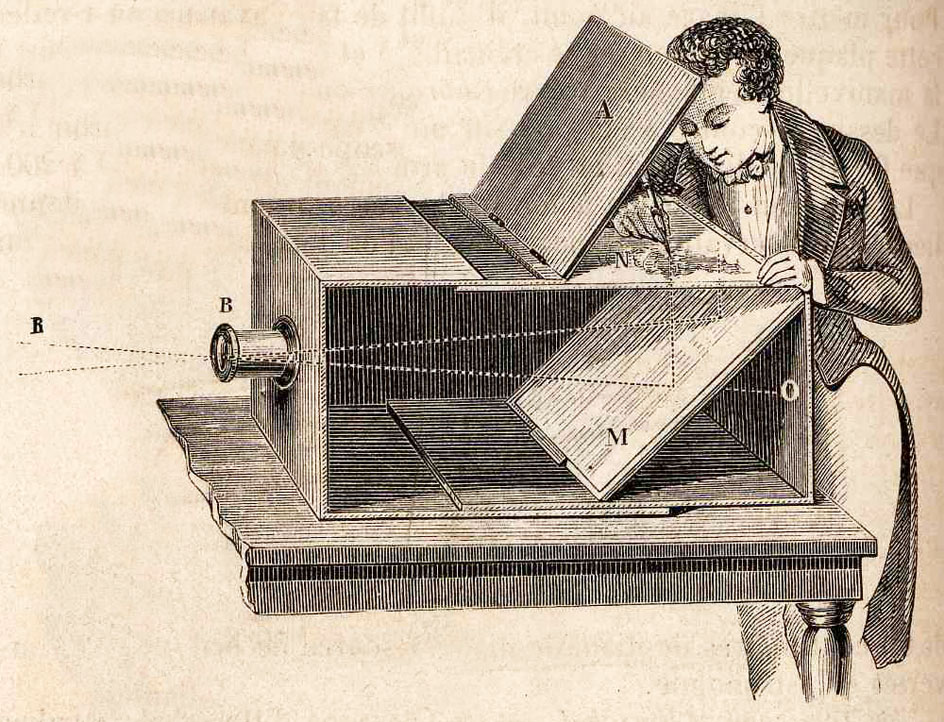
\includegraphics[width= 0.7\columnwidth]{images/contestoRiferimento/01_cameraOscura.jpg}
		\caption{Immagine della Camera Oscura.}
		\label{fig:contesto_riferimento_camera_oscura}
	\end{figure}
	
	Parallelamente, si intuiscono le possibili applicazioni del fenomeno in ambito artistico: diventa così oggetto di studio in tutto il filone di ricerca sulla prospettiva pittorica.”
	Nel Seicento fu creato un modello portatile di camera oscura, definita \textit{reflex}, In Figura~\ref{contesto_camera_oscura} ne viene mostrato il funzionamento. Prevedeva l’utilizzo di uno specchio inclinato che rifletteva l’immagine su una superficie di vetro sulla quale era possibile disegnare. Naturalmente l’utilizzo di questo strumento divenne ben presto una consuetudine nella pratica pittorica poiché consentiva all’artista di disegnare la realtà così come appariva sul vetro e in seguito rappresentò un fondamentale riferimento per tutti gli apparecchi fotografici.
	
	\item \textbf{Lanterna Magica.}
	\label{contesto_lanterna_magica}
	Antenata del moderno proiettore cinematografico, la Lanterna Magica è un apparecchio dotato di un sistema ottico e di una fonte di luce che proietta, ingrandite su uno schermo o su una parete bianca, immagini raffigurate su vetro.
	
	Il sistema ottico prevede un riflettore, un condensatore e un obiettivo: il riflettore, uno specchio concavo posizionato dietro la fonte di luce, raccoglieva i raggi luminosi e li direzionava verso il condensatore, un sistema di lenti che aveva la funzione di convergere i raggi sull’immagine dipinta e rinviarli all’obiettivo che infine proiettava l’immagine ingrandita sullo schermo.
	Il riflettore, la sorgente luminosa e il condensatore erano collocati all’interno della macchina, una semplice scatola con un camino per la fuoriuscita del fumo prodotto dalla fonte di luce; l’obiettivo era invece collocato all’esterno, sulla parte anteriore della lanterna e consentiva l’inserimento di lastre di vetro dipinte.
	In Figura~\ref{contesto_lanterna_magica} si può osservare la Lanterna Magica ed uno schema del suo funzionamento.
	
		\begin{figure}%[h]
			\centering
			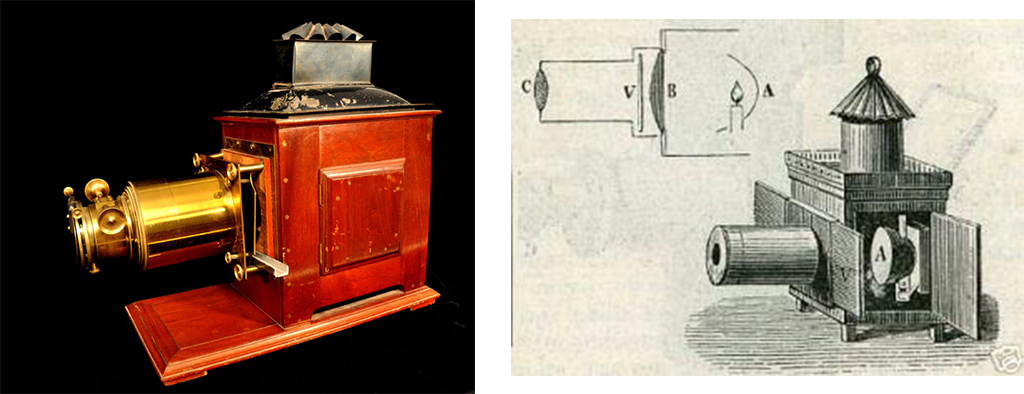
\includegraphics[width= 0.8\columnwidth]{images/contestoRiferimento/02_lanterna.jpg}
			\caption{Immagine della Lanterna Magica e schema di funzionamento.}
			\label{fig:contesto_riferimento_lanterna_magica}
		\end{figure}
	
	Nata nel Seicento barocco, la Lanterna Magica si diffuse in brevissimo tempo in ambiti e paesi diversi connotandosi come una macchina da spettacolo al momento stesso della sua comparsa. Pur nascendo come dispositivo fondato su precise leggi scientifiche, la nuova invenzione finì ben presto per apparire magica e sovrannaturale agli occhi del popolo, poiché capace di suscitare stupore, meraviglia ed emozioni profonde negli spettatori, soprattutto i meno istruiti. Per la prima volta era possibile osservare immagini a colori e in movimento che comparivano dal nulla con un effetto prodigioso, a tal punto che spesso il pubblico aveva la sensazione di poter “toccare con mano” quelle immagini favolose. Immagini che potevano apparire addirittura miracolose per gli spettatori che le osservavano senza capire il meccanismo. Non dimentichiamo che all’epoca nessuno aveva mai assistito prima ad uno spettacolo simile poiché nessuna forma di rappresentazione preesistente (come quadri, statue e affreschi) era in grado di simulare la vita e il suo movimento.
	
	Nel corso dei secoli la Lanterna venne utilizzata nei modi più diversi, non soltanto come strumento spettacolare ma anche come efficace mezzo educativo. Nel ‘600, ad esempio, il padre gesuita Kircher sfruttò le qualità prodigiose della Lanterna Magica finalizzandole all’educazione e cristianizzazione degli spettatori adoperandola come efficace strumento di evangelizzazione comprensibile a tutti, con una forza di persuasione e una potenza visiva senza precedenti. Nell’800 venne inoltre utilizzata anche in ambito scientifico e come efficace strumento per divertire istruendo e istruire divertendo. Sfruttando, ad esempio, la sua capacità di ingrandire le immagini al punto di proiettare una mosca grande come un elefante, la lanterna magica venne trasformata in un vero e proprio microscopio.
	
	\item \textbf{Dissolving Views.}
	\label{contesto_dissolving_views}
	Tra i vari utilizzi spettacolari legati alla Lanterna Magica vennero studiate raffinate tecniche di proiezione come gli incredibili effetti di dissolvenza. La nuova tecnica si basava sull’uso combinato di due o più lanterne affiancate che proiettavano, sul medesimo punto dello schermo, la graduale apparizione di un’immagine sovrapposta a quella precedente che, a poco a poco, scompariva. Spesso i soggetti proposti erano complementari riuscendo così a mostrare ad esempio il passaggio delle stagioni su un medesimo paesaggio dipinto. Vennero inoltre utilizzati particolari otturatori, diffusi in modelli diversi che consentivano di coprire gradualmente l’obbiettivo della prima lanterna e, contemporaneamente, di scoprire quello della seconda. Grazie a questo gioco di alternanza, i soggetti si \textit{dissolvevano} uno nell’altro.
	
\end{itemize}

\subsection{Situazione museale}
\label{sec:situazione_museale}

Il contesto museale ed il pubblico, che usufruisce del servizio fornito dai musei italiani, stanno pesantemente cambiando negli ultimi decenni.
L’indagine “Il museo in ascolto. Nuove strategie di comunicazione per i musei statali”, svolta da Ludovico Solima presentata nel Giugno del 2012 all’Istituto Nazionale per la Grafica di Roma \cite{MuseoInAscolto}, mostra il triplicarsi di presenze di anziani ed il dimezzamento del numero di ragazzi che si avvicinano alle strutture museali.
Il lavoro di Solima è stato svolto tra il Dicembre del 2010 e Giugno 2011 con più di 4500 questionari distribuiti in 12 musei statali italiani.

Secondo Solima, il pubblico chiede una maggiore partecipazione e non vuole più essere esclusivamente fruitore di contenuti. Con lo sviluppo di internet è pesantemente cambiato anche il paradigma di comunicazione. Attualmente il contatto tra il pubblico giovane e la struttura museale avviene principalmente in rete, e solo in maniera secondaria in forma cartacea e tramite passa parola.
La ricerca evidenzia che il 46\% del pubblico giovane effettua la visita con i propri genitori e solo il 17\% da solo. “Molto importante è l'esigenza di una \textit{visione d'insieme} che il museo dovrebbe contribuire a fornire, rispetto alla specificità dell'opera. Ciò implica il passaggio da una lettura del museo di tipo enciclopedico, ad una di tipo narrativo, attraverso una nuova strategia comunicativa che si basi più sul racconto e meno sul dato.”

Negli ultimi anni, in Italia, sono stati presi numerosi provvedimenti in direzione di un avvicinamento del pubblico più giovane al contesto museale, come l’entrata gratuita per gli Under-18 o l’apertura di alcuni musei durante le ore notturne. Ciò che emerge dai dati è comunque un'evidente mancanza di interesse nei confronti dei musei, dovuta anche alla diffusione dell’informazione su media differenti, che incentivano il pubblico ad avvicinarsi in maniera ridotta a luoghi culturali tradizionali, musei, parchi archeologici e complessi monumentali.

Secondo i dati Istat dell'annuario statistico italiano 2013 \cite{DatiIstatMusei} il 42,2\% dei giovani di età compresa tra gli 11 ed i 14 anni ed il 33\% di quelli tra i 15 e 17 anni ha visitato almeno un museo durante l’anno 2013. Sono dati che possono essere letti in maniera preoccupante soprattutto se si considera il fatto che la maggior parte delle entrate registrate sono state fatte tramite visite scolastiche. Le iniziative, in ambito didattico, permettono ai giovani di avvicinarsi ai musei ed ai luoghi culturali, ma difficilmente aumentano l’interesse dei giovani nei confronti dei beni culturali che visitano.  

\section{Contesto aziendale}
\label{sec:contesto_aziendale}

\subsection{Azienda}
\label{sec:azienda}

e-Mentor nasce nel 2004 a Torino per iniziativa dell’Ing. Manuela Martini, caratterizzandosi sin dal principio per l’attenzione alla ricerca e all’innovazione tecnologica, come attestato dai premi \textit{“Galileo Ferraris”} e \textit{“e-Content Award of Italy”}. 

Durante questi 10 anni, e-Mentor si è distinta come leader nel campo di soluzioni innovative per istituzioni, organizzazioni e aziende in ambito \textit{e-learning}, \textit{web \& mobile design}, \textit{edutainment} e \textit{software engineering}.

Nell’ambito del \textit{Mobile Design}, e-Mentor progetta e realizza applicazioni ad alta interattività per smartphone e tablet, fruibili su piattaforme iOS, Android e Windows. Attraverso l’impiego delle più aggiornate tecnologie mobili, vengono sfruttate le potenzialità del mobile computing per progettare soluzioni innovative, che spaziano dal \textit{learning on the move} - per offrire contenuti e servizi formativi interattivi in modo sempre più mirato e versatile, al \textit{situated content} - creando percorsi didattici basati sull'esplorazione del territorio con contenuti localizzati e specifici, sino agli \textit{advergames} – ideando giochi e applicativi collegati a brand ed iniziative di marketing, oppure a scopo didattico-educativo.

Grazie all'esperienza maturata nel \textit{media \& interaction design}, il team di e-Mentor progetta e sviluppa soluzioni \textit{Game-Based Learning}, quali \textit{serious games} e simulazioni interattive per facilitare l'utente nella rapida acquisizione di competenze tecniche, relazionali e organizzative attraverso il paradigma apprendimento-gioco.

Inoltre, relativamente all’ambito \textit{Web} e \textit{Software Engineering}, e-Mentor propone soluzioni web-based e stand-alone personalizzate, realizzate con tecnologie quali Php, Mysql, Java, J2ME, Ajax, in settori di applicazione come il retail, l’health care, la didattica e per ogni possibile utilizzo custom per il settore privato e pubblico.

\subsection{Situazione del progetto precedente al nostro inserimento}
\label{sec:azienda_precedente}

Il Museo del Cinema di Torino, da tempo pone l’attenzione al problema della poca affluenza di ragazzi in età adolescenziale, cercando soluzioni originali che possano invertire questa tendenza (Capitolo \ref{sec:contesto_museale}).

La collaborazione tra e-Mentor e Museo del Cinema nasce, nel 2013, per provare a porre rimedio a questo problema.
Tra le prime soluzioni proposte c’è quella di sviluppare un videogioco che avvicini i ragazzi a tematiche trattate all’interno del Museo. In seguito a mesi di lavoro e riunioni tra esperti dell’ambito \textit{learning}, artistico e del videogame, viene prodotto un documento di Design, che contiene idee di meccaniche, ambientazioni e scenari di gioco. Le tematiche che si è deciso di trattare sono quelle del \textit{pre-Cinema}, caratterizzato da tecnologie, oggettistica e curiosità per lo più ignoti al pubblico.
Il documento di Design viene presentato al bando \textit{Creative Europe, MEDIA Sub-programme, Support for Concept and Project Development of Video Games}, del Marzo 2014 \cite{CreativeEurope}.
L’idea di Design viene accolta positivamente, ma la domanda viene scartata perché il progetto viene considerato poco definito, con alcuni elementi di \textit{gameplay} non adatti ad essere finanziati e quindi lanciati sul mercato.

\subsection{Inserimento in azienda}
\label{sec:azienda_inserimento}

I nostri primi contatti con e-Mentor sono avvenuti tra Novembre e Dicembre 2014. Durante i primi incontri ci si è dedicati soprattutto all'analisi del progetto \textit{The Magic Lantern}, allo studio del contesto ed alla comprensione delle possibilità di re-design del lavoro precedentemente svolto.
Si è poi proseguito con la creazione di una timeline dettagliata di tutte le fasi di lavoro, si può far riferimento al Capitolo~\ref{sec:dev_fasi_sviluppo} per ulteriori dettagli a riguardo.
e-Mentor si è quindi fatta carico di fornirci documentazione e strumenti adeguati all'analisi del contesto, in modo da poter affrontare ogni fase del lavoro in maniera preparata ed efficiente.
Durante lo sviluppo del progetto abbiamo organizzato dei meeting periodici, ogni 3-4 settimane, con l'azienda ed esperti del settore, per ottenere linee guida sul proseguimento del lavoro, oltre che utili consigli soggettivi.

\chapter {Ruolo del Videogame e Stato dell'Arte}
\label{chap:gaming_layer}

\section{Gaming Layer}

\subsection{Statistiche ed Evoluzione}

Una delle forme di intrattenimento più famose e usate al giorno d'oggi sono i videogame. Secondo i dati esposti nel report ESA 2014, l'età media dei videogiocatori è di 31 anni, e il 48\% di questi è di sesso femminile \cite{esareport-stats}.
Il numero di donne sopra i 50 anni che giocano ai videogame è aumentato del 32\% dal 2012 al 2013, in generale i gamer adulti hanno giocato per una media di 16 anni (nel dettaglio, gli adulti maschi hanno una media di 18 anni mentre le donne arrivano a 13) \cite{seriousgamingementor}.

\begin{figure}[h]
\centerline{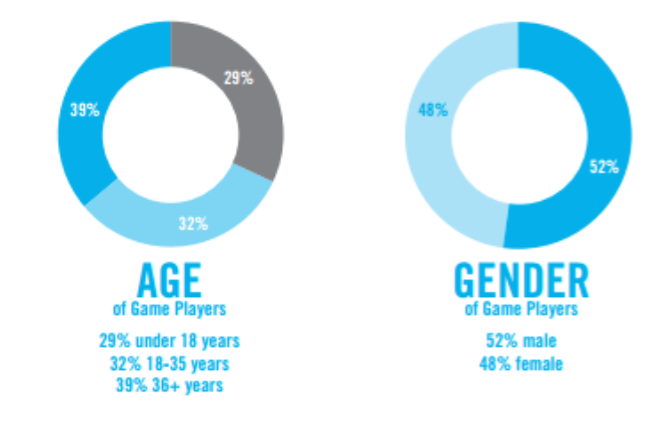
\includegraphics[scale=0.45]{images/statoarte/statsgamers.png}}
\caption{Statistiche sui videogiocatori.}
\label{fig:statsgamers}
\end{figure}

All'età di 21 anni, una persona abituata a giocare ai videogame, avrà già collezionato più di 10.000 ore di gioco, il che corrisponde a 40 ore a settimana per 5 anni, stesso tempo che un normale studente dedica alla scuola superiore \cite{seriousgamingementor}.

Questa situazione non sarebbe stata possibile anni fa, quando le reti di comunicazione non erano ancora così presenti nella vita quotidiana delle persone, le quali hanno quindi catalizzato la diffusione della cultura del videogame. Un altro fattore, che ha dato una spinta alla diffusione dei videogame, è certamente la presenza dei Social Network (come Facebook), i quali facilitano la diffusione dei cosidetti giochi ``virali'', cioè quei giochi che, fra le varie meccaniche, ne hanno una che prevede la diffusione del gioco tramite passaparola dei giocatori, i quali traggono spesso dei vantaggi dal fare questa azione (per esempio il bonus di 1 vita extra per il gioco Candy Crash Saga). E' quindi innegabile il potenziale divulgativo che possiede un videogame.

Ma il videogioco non è solo una forma di intrattenimento, secondo molti ricercatori rappresenta qualcosa di più.
Come si afferma in un articolo del sito ``PsychCentral'' \cite{phychcentral}, i giochi Sparatutto tendono a migliorare le skill cognitive come la navigazione spaziale, il ragionamento, la memoria e la percezione. 
Altri giochi più strategici (come i giochi di ruolo, o i puzzle solving) tendono a far sviluppare skill come il problem solving, per non parlare del multitasking che viene costantemente messo a dura prova in moltissimi giochi di abilità.


Detto ciò, è ragionevole considerare il videogame come mezzo di apprendimento e miglioramento. Per grandissima parte dei giochi questo apprendimento è stata una conseguenza ``non prevista'' da parte degli sviluppatori, 
in quanto il core principale dei giochi è sempre stato il solo intrattenimento. Esiste però una categoria di giochi il cui obiettivo non è solamente l'intrattenimento, ma anche il trasmettere altri concetti, come l'educazione o l'informazione riguardo una certa tematica, o addirittura il fornire un training riguardo un certo ambito (fornendo quindi delle volte una vera e propria simulazione al giocatore). Questa categoria di videogame si chiama ``Serious Game''.

\subsubsection{Theory of Fun}

Accanto ai Serious Game, esiste un altro metodo che si basa sui principi dei giochi, questa è la Gamification (per una distinzione dettagliata fra Gamification e Serious Game fare riferimento al Paragrafo \ref{sec:distinzioni}).

Un esempio di Gamification è stata l'installazione di una tastiera musicale sulla scalinata dell'uscita di una metropolitana. Le persone, attratte e divertite dalla musica prodotta dal loro passaggio sugli scalini, preferivano usare le scale tradizionali piuttosto che le scale mobili. Alla fine si è riscontrato un aumento del 66\% delle persone che hanno preferito le scale tradizionali a quelle mobili.

Un secondo esempio ha riguardato i bidoni dell'immondizia di un parco: sono stati installati dei sensori, che all'arrivo di un rifiuto al proprio interno, facevano partire il suono tipico di un oggetto che cade per centinaia di metri nel vuoto. Questa semplice installazione ha attratto la curiosità di molti passanti, i quali, incuriositi e ignari della parte artificiale di tutto ciò, buttavano i rifiuti dei dintorni pur di sentire di nuovo quello strano suono e capirne qualcosa in più.

Questi scenari sono stati creati per un concorso indetto da Volkswagen, chiamato ``Theory of fun'', nel quale si afferma: ``Qualcosa di tanto semplice come il divertimento rappresenta il modo più semplice per cambiare il comportamento delle persone in meglio''.

Sia i Serious Game che gli esperimenti di Gamification sono in linea con il nostro obiettivo, cioè spronare un certo pubblico ad interessarsi a luoghi di culto come i musei (nel nostro caso in particolare, il Museo del Cinema). Come abbiamo già detto, e rivedremo meglio nei prossimi capitoli, fra i due approcci si è scelto quello del Serious Game per lo sviluppo del progetto \manclass{The Magic Lantern}.

\newpage

\subsection{Serious Game}

\subsubsection{Cosa Sono}
\label{sec:cosasono}

L'origine dei giochi a scopo formativo viene generalmente ricondotta alle simulazioni di guerra (''Kriegsspiel'') dell'esercito prussiano degli inizi del XVIII secolo.
Il termine Serious Game venne probabilmente usato la prima volta da Clark Abt, sviluppatore di giochi militari su computer, nel 1971. Nel suo libro ``Serious Game'', il ricercatore statunitense fornisce anche una definizione dei giochi educativi, a prescindere dal supporto (digitale o real-world). Li descrive come giochi con un esplicito e ben strutturato scopo educativo, non pensati primariamente per il divertimento, senza però escluderlo \cite{wikiseriousgames}.
Nonostante la nascita di questi sia ormai datata, la loro diffusione sta aumentando soprattutto negli ultimi anni, grazie anche alle nuove tecnologie per lo sviluppo di videogame.

E' possibile identificare alcuni ambiti in cui i Serious Game agiscono, per esempio gli autori del sito \url{www.serious.gameclassification.com} \cite{seriousclass} hanno stabilito la seguente tassonomia: 

\begin{itemize}
\item Educative message broadcasting 
\item Informative message broadcasting
\item Marketing \& Communication message broadcasting
\item Subjective message broadcasting
\item Training
\item Goods trading
\item Storytelling
\item Licensed title
\end{itemize}

Sempre gli stessi autori hanno contribuito a varie conferenze e articoli scientifici sui Serious Game, disponibili sempre sul loro sito \cite{seriousclass}.


\subsubsection{Serious Game e altre forme di intrattenimento simili}
\label{sec:distinzioni}

Come già detto, il Serious Game non è l'unica forma di intrattenimento che si basa sul gaming (\myfig{\ref{fig:gameschema}}). 

\begin{figure}[h]
\centerline{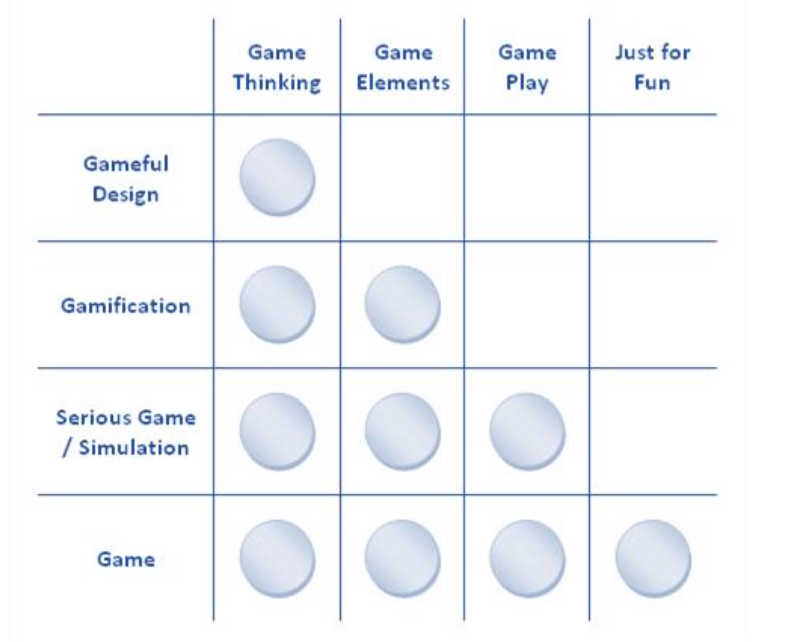
\includegraphics[scale=0.3]{images/statoarte/gameschema.png}}
\caption{Diversi approcci al gaming.}
\label{fig:gameschema}
\end{figure}

Possiamo distinguere 4 categorie:

\begin{itemize}
\item Gameful Design: ha una funzionalità spesso meramente estetica, difatti non ci sono elementi di gioco, ma il design ne ricorda il game thinking. Per esempio Twitter ha usato delle pagine molto particolari (al posto della tipica pagina con error 404) per casi in cui una pagina del sito non venga trovata \myfig{\ref{fig:gamefuldesignex}}.

\begin{figure}[h]
\centerline{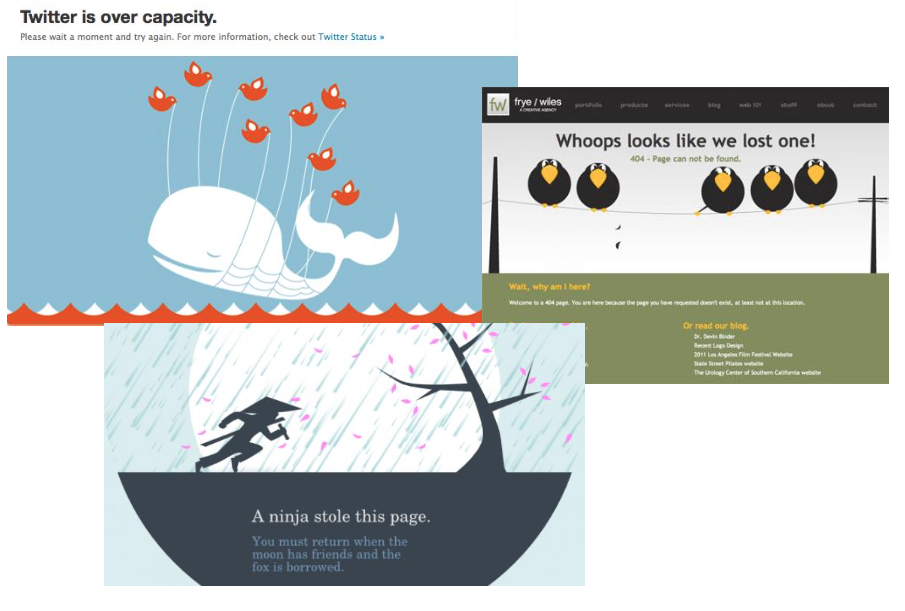
\includegraphics[scale=0.35]{images/statoarte/gamefuldesignex.png}}
\caption{Esempi di Gameful Design.}
\label{fig:gamefuldesignex}
\end{figure}

\item Gamification: contiene alcune delle meccaniche oltre che tipici elementi di gioco, come l'assegnazione di punti o il raggiungimento di livelli. Per esempio Dropbox ha creato una competizione fra gli atenei Universitari, dove l'obiettivo (per Ateneo) era raggiungere il numero più alto di iscritti. La ricompensa per gli studenti consisteva in GB gratis tramite il medesimo servizio di cloud \myfig{\ref{fig:gamefuldesignex}}.

\begin{figure}[b]
\centerline{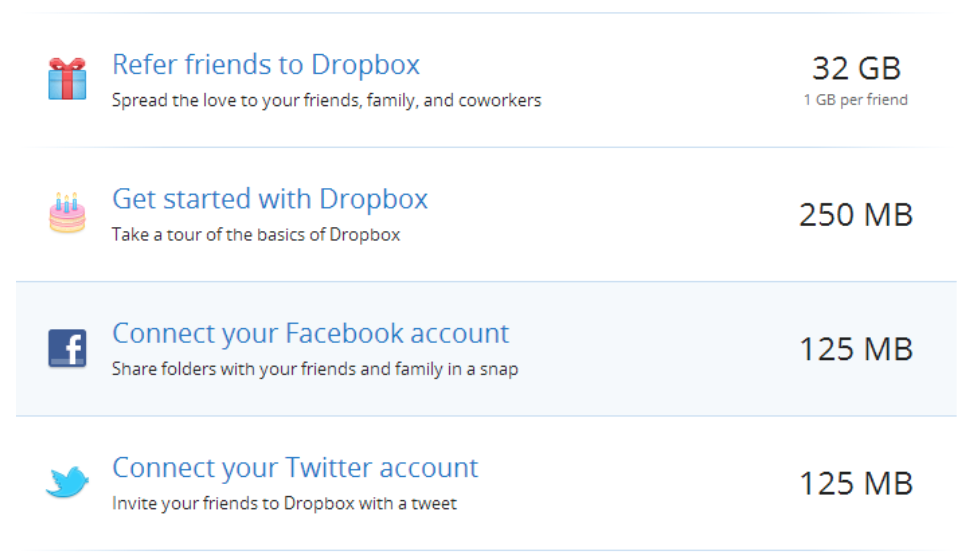
\includegraphics[scale=0.3]{images/statoarte/gamificationex.png}}
\caption{Esempio di Gamification.}
\label{fig:gamificationex}
\end{figure}

\item Serious Game: possiede tutte le caratteristiche di un videogame, il cui scopo però non è il solo divertimento. Per esempio, un Serious Game chiamato Dragon Box, si propone di insegnare l'algebra a dei bambini tramite dei rompicapo \cite{dragonboxhome}.


\item Game: sono i tipici videogame il cui obiettivo è solamente divertire e intrattenere il pubblico.
\end{itemize}

Il nostro prodotto si classifica come Serious Game in quanto presenta meccaniche pure di un videogame, quali platoform e rompicapo (che vedremo nel Capitolo \ref{chap:game_design} sul Game Design), ma in più ha lo scopo di incuriosire il pubblico verso la tematica del pre-cinema.

\newpage

\subsubsection{Approccio Esperienziale}
\label{sec:seriousgameesp}

Come afferma Wikipedia \cite{wikiseriousgames}, non esiste una teoria uniforme sulla pedagogia dei Serious Game. Se in passato i giochi erano basati sulla psicologia comportamentale, come ad esempio nel gioco Mathblaster  \cite{mathblaster}, 
oggi gli sviluppatori di videogiochi educativi attingono da vari modelli pedagogici e particolare importanza ha assunto l'apprendimento esperienziale che parte dal presupposto che le informazioni 
e le sensazioni vissute rimangono fortemente impresse e permettono in questo modo al giocatore di affinare percezione, attenzione e memoria favorendo modifiche comportamentali attraverso il learning by doing (``imparare facendo'').

Uno dei punti di forza che ha il videogame nel fattore apprendimento consiste nella semplice interazione che si richiede all'utente. Come si può apprendere dalla relativa pagina su Wikipedia \cite{apprendimentoesperienziale}, questo modello di apprendimento si chiama esperienziale, e come suggerisce il nome, si basa sull'esperienza, sia essa cognitiva, emotiva o sensoriale. Il processo di apprendimento si realizza attraverso l'azione e la sperimentazione di situazioni, compiti, ruoli in cui il soggetto, attivo protagonista, si trova a mettere in campo le proprie risorse e competenze per l'elaborazione e/o la riorganizzazione di teorie e concetti volti al raggiungimento di un obiettivo. L'apprendimento esperienziale consente al soggetto di affrontare situazioni di incertezza sviluppando comportamenti adattivi e migliorando, nel contempo, la capacità di gestire la propria emotività nei momenti di maggiore stress psicologico. Consente inoltre di sviluppare le proprie abilità di problem solving, anche attraverso l'abilità creativa, e di far acquisire autoconsapevolezza mediante auto-osservazione ed etero-osservazione al fine di ridefinire eventuali atteggiamenti inadeguati e di valorizzare i comportamenti costruttivi. L'esperienza così acquisita diviene patrimonio di conoscenza del soggetto e costituirà il nuovo punto di partenza di ulteriori evoluzioni.

Questo approccio non è recente, e uno studio condotto a Washington \cite{vreduchristine} (risalente al 1996) ha raccolto dei dati interessanti sfruttando anche questa metodologia.
Questo studio mirava a capire quanto la realtà virtuale unita al videogioco potessero migliorare il grado di apprendimento dello studente, per esempio nel caso di un laboratorio di chimica. L'esperimento è stato condotto in varie modalità di apprendimento (solo le ultime 2 sfruttano l'approccio esperienziale): 

\begin{itemize}
\item semplice lezione,
\item lezione in videocassetta, 
\item gioco su pc, 
\item gioco con supporto di realtà virtuale.
\end{itemize}

Ciò che è stato dedotto tramite vari test effettuati sugli studenti è che l'apprendimento della lezione è in media superiore nei casi dove è richiesta una interazione (gioco pc, gioco in realtà virtuale). La statistica è stata a favore di queste categorie non solo per i test effettuati subito dopo i training, ma lo è stata anche e soprattutto per i test effettuati settimane dopo, ciò vuol dire che il ``fattore interazione'' tende a far apprendere stimolando non solo la memoria a breve termine ma anche quella a lungo termine.

Un altro fattore, molto affine all'approccio esperienziale, che rientra fra le caratteristiche dei giochi, è il ``trial-and-error'' come metodo per il problem-solving. Il trial-and-error \cite{trialanderror} ha varie caratteristiche: 

\begin{itemize}
\item Solution-oriented: questo approccio non cerca di capire perché una soluzione funzioni, ma si basa sul fatto che questa sia una soluzione;
\item Problem-specific: non si cerca di generalizzare una soluzioni ad altri problemi;
\item Non-optimal: si trova in genere una soluzione, non la soluzione migliore;
\item Needs little knowledge: questo metodo è perfetto soprattutto se si ha poca o nessuna conoscenza riguardo un ambito.
\end{itemize}

Dei famosi utilizzi di questo approccio sono avvenuti in ambito medico, con la scoperta degli antibiotici per esempio \cite{trialanderror}. Oggigiorno questo approccio è praticamente alla base di ogni videogame, dove il giocatore si appresta a scoprire sempre qualcosa di nuovo, e grazie a questo approccio ci si sente liberi di poter fallire e riprovare serenamente, finché non si sarà appreso la ``lezione'', la quale può consistere nel capire la giusta sequenza di tasti per sconfiggere un nemico, ma può anche consistere nell'apprendere come condurre un'esperimento chimico in tutta libertà e sicurezza.

\newpage

%--------------------------
%--------------------------

\section{Stato dell'arte}
\label{chap:stato_dell_arte}

\subsection{Giochi di interesse per il nostro caso di studio}

Come già detto, il nostro caso di studio ha come obiettivo la diffusione di informazioni riguardanti il pre-cinema, allo scopo di attrarre l'attenzione dei più giovani verso questa tematica e con la speranza che una certa percentuale di questi voglia quindi approfondire le loro conoscenze visitando il Museo del Cinema di Torino.

Per raggiungere questi obiettivi, il game design originale del gioco \manclass{The Magic Lantern} prevedeva un gameplay diviso a metà fra i generi platform e puzzle (rompicapo). E' stato quindi condotto uno studio sullo stato dell'arte di videogame appartenenti a queste due categorie, oltre che appartenenti alla tipologia Serious Game. In particolare, ci si è concentrati su Serious Game di tipo ``Informative message broadcasting'', i quali hanno appunto lo scopo di diffondere un certo tipo di messaggio, nel nostro caso sarebbe appunto l'esistenza delle tecnologie appartenenti al pre-cinema e quindi la loro storia.

Vediamo quindi di analizzare i singoli giochi che sono stati ritenuti utili per il nostro studio.

%--------------------------

\subsection{Valiant Hearts}

Valiant Hearts è un Serious Game ambientato nella prima guerra mondiale, il cui scopo è, oltre che divertire il player, far scoprire all'utente vari dettagli riguardo quel particolare periodo storico.

Il gioco ha delle meccaniche di tipo platform/avventura e puzzle (rompicapo): 

\begin{itemize}
\item platform/avventura poiché il mondo è esplorabile (tramite porte, piattaforme etc) e poiché sono presenti dei collezionabili da raccogliere; 
\item rompicapo perché alcune sezioni richiedono la risoluzione di alcuni indovinelli per essere superate.
\end{itemize}

Vediamo nella \myfig{\ref{fig:vhgameplay}} uno screenshot del gameplay del gioco. 

\begin{figure}[h]
\centerline{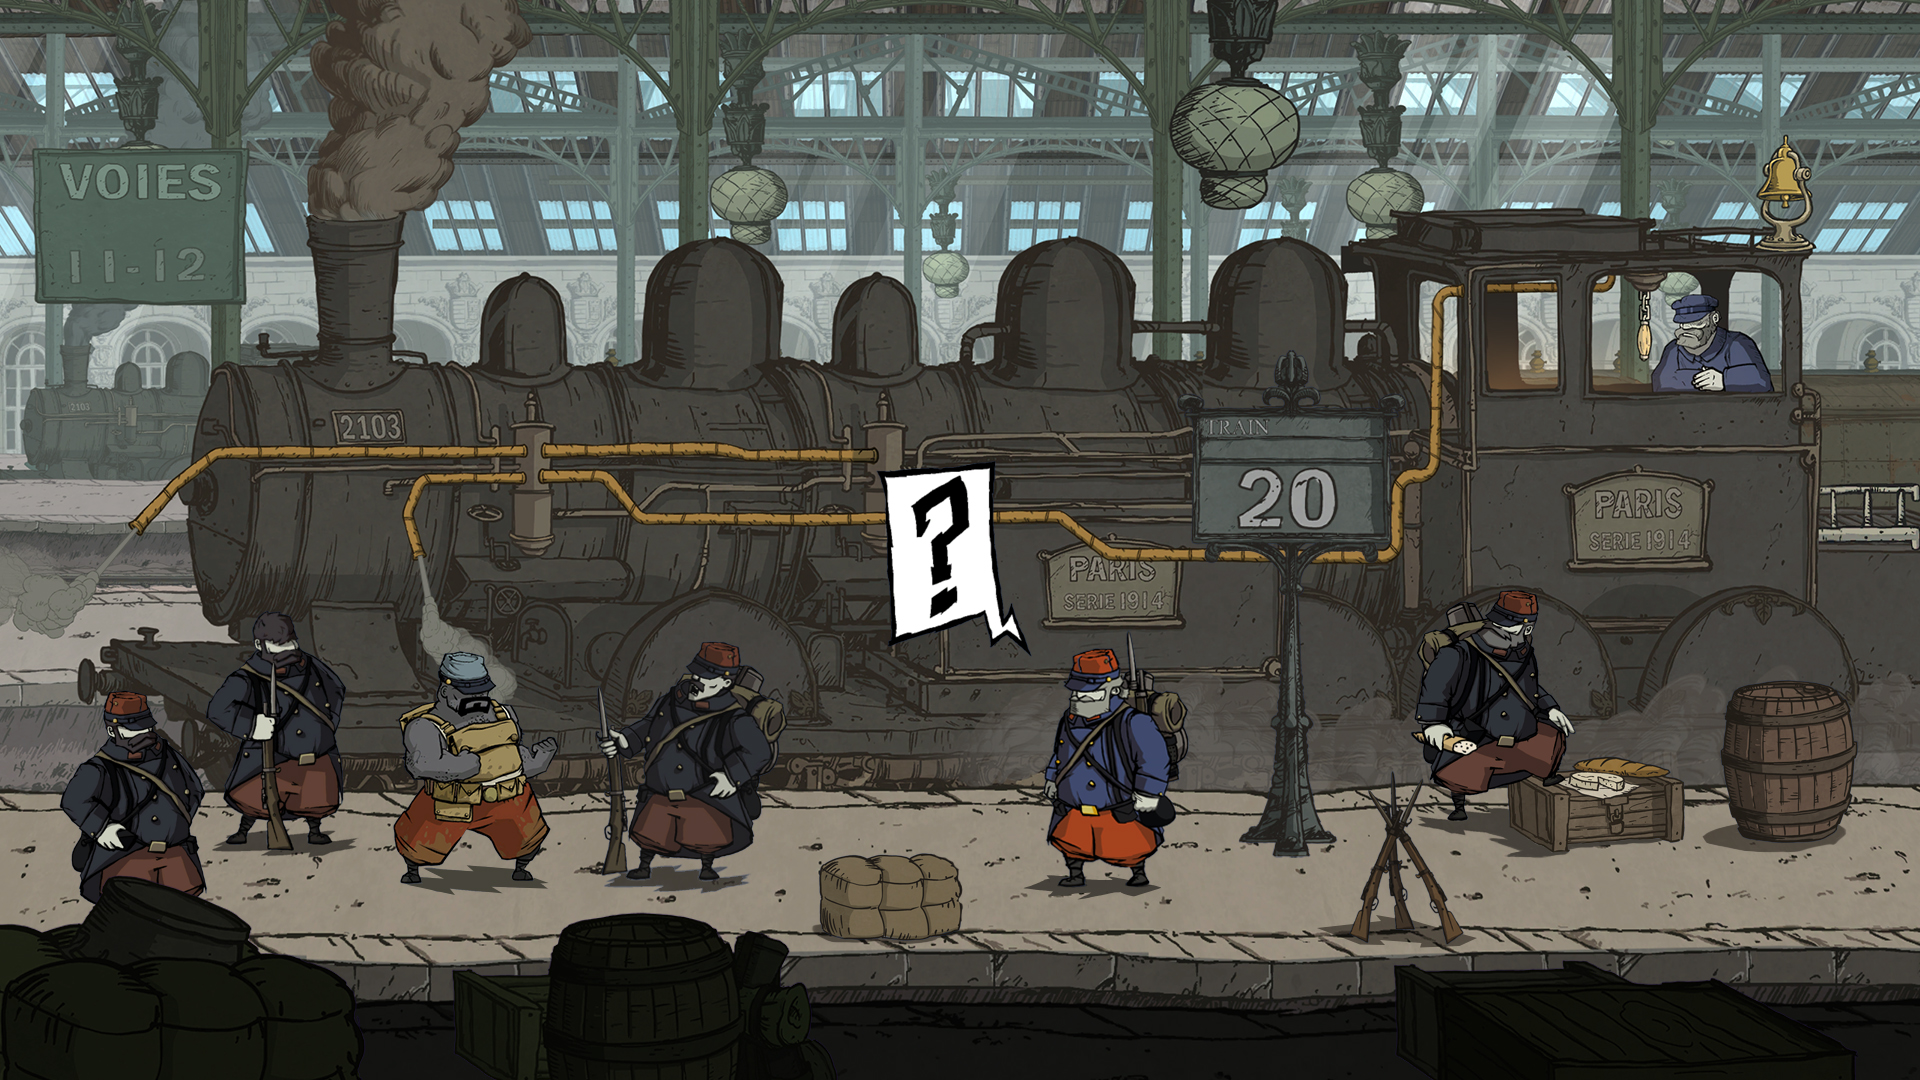
\includegraphics[scale=0.17]{images/statoarte/vhgameplay.jpg}}
\caption{Gameplay di Valiant Hearts.}
\label{fig:vhgameplay}
\end{figure}

Entrambe le tipologie di gioco favoriscono la parte Serious dell'esperienza:

\begin{itemize}
\item La parte platform aiuta in quanto ad ogni collezionabile preso viene sbloccata la corrispettiva scheda informativa, che spiega i dettagli storici riguardo quell'oggetto. Per esempio, la raccolta di una maschera a gas sblocca una scheda che narra dei primi attacchi batteriologici usati durante la prima guerra mondiale, oppure dopo aver raccolto una medaglietta da soldato dell'esercito, se ne spiegano i dettagli storici.
\item Alcune delle sezioni rompicapo sono collegate alle schede informative sbloccate, ciò invoglia il giocatore ad informarsi a riguardo. Per esempio durante un livello è presente una sezione con dei tubi che perdono gas letale, per superare questa sezione va risolto un indovinello. Proprio poco prima di questa sezione, l'utente ha avuto la possibilità di raccogliere l'oggetto maschera a gas e quindi di sbloccare la relativa scheda informativa.
\end{itemize}

Osservando la \myfig{\ref{fig:vhUIFacts}} è possibile capire come avvenga la fruizione di contenuti Serious del gioco. Una volta ottenuto un oggetto, si bloccherà il relativo ``Fatto'', leggibile da questa interfaccia, alla quale si può accedere in ogni momento di gioco.
La disposizione prevede: un menù di navigazione disposto in verticale sulla sinistra; una immagine rappresentativa del fatto storico posta in alto al centro; la descrizione del fatto storico in basso al centro.
\begin{figure}[h]
\centerline{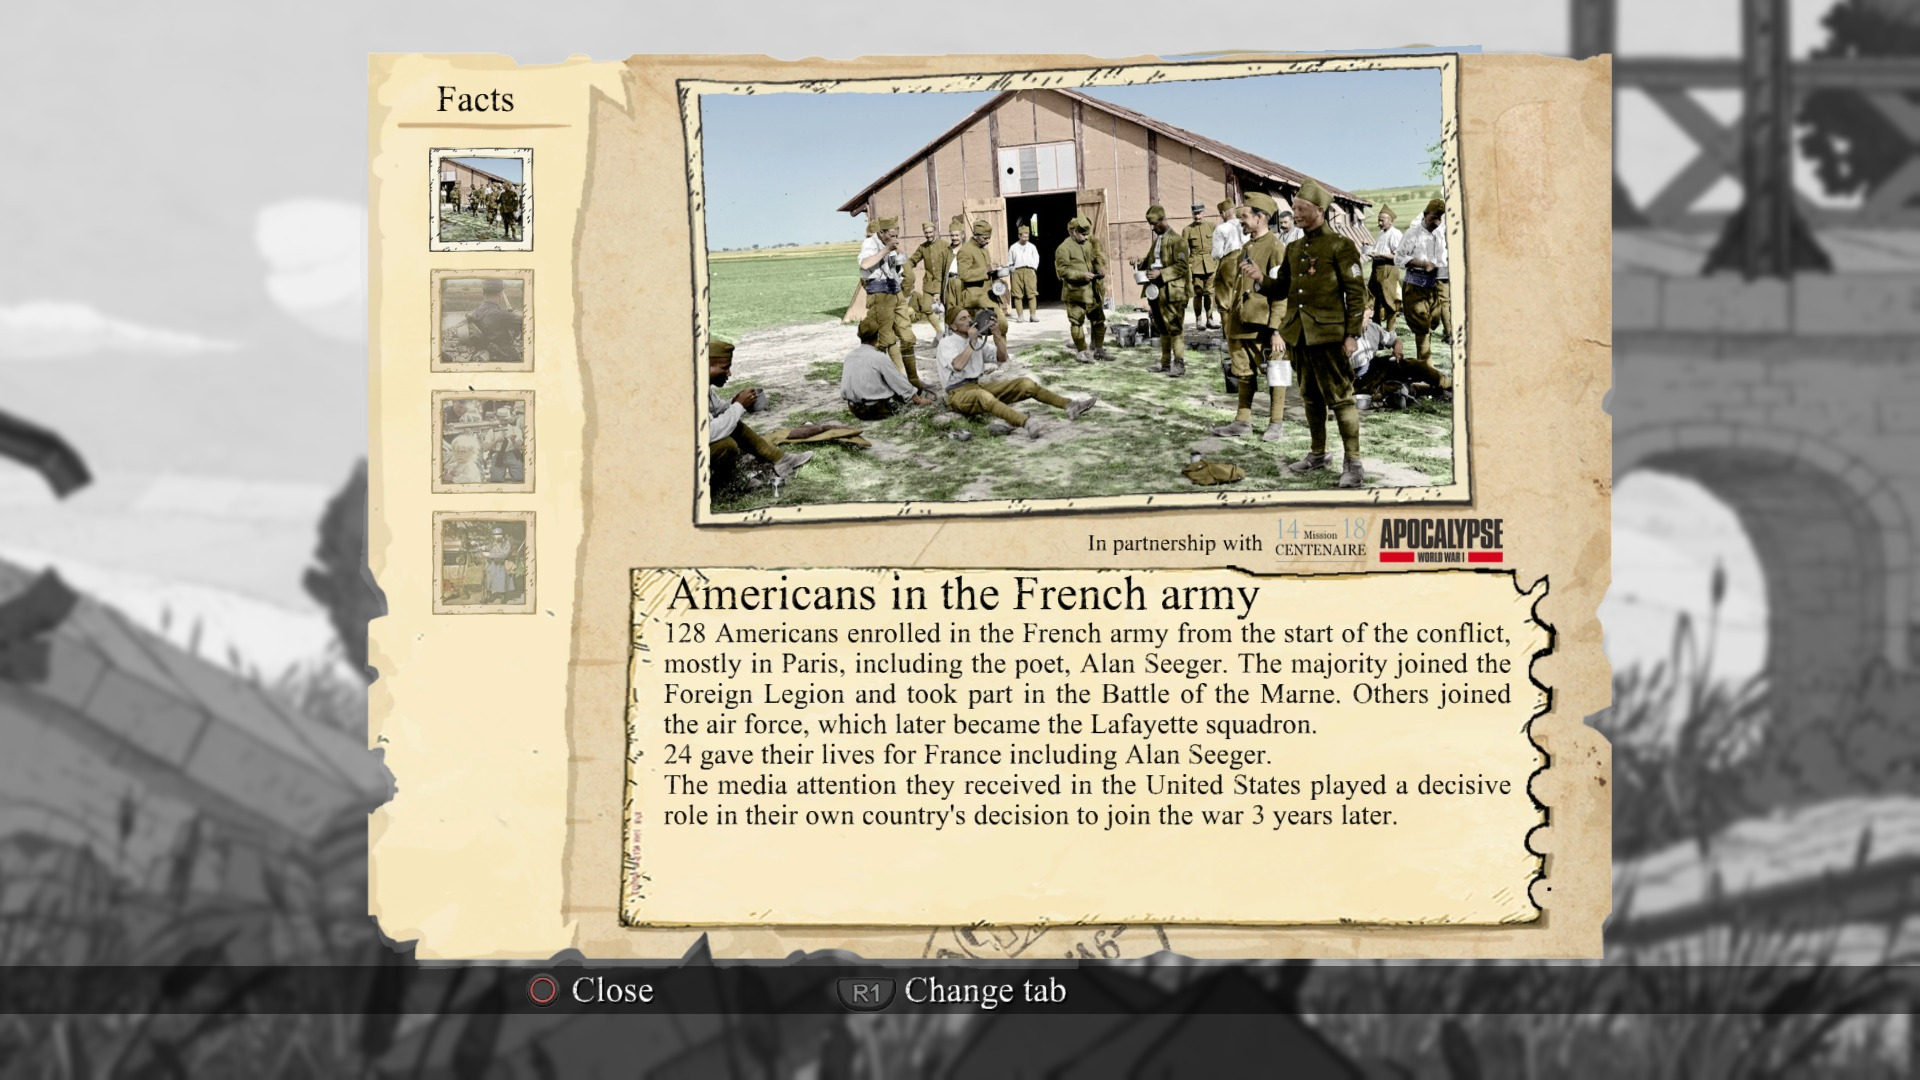
\includegraphics[scale=0.22]{images/statoarte/vhUIFacts.jpg}}
\caption{Menù dei contenuti Serious di Valiant Hearts.}
\label{fig:vhUIFacts}
\end{figure}

Gli sviluppatori (Ubisoft Montpellier) hanno scelto di produrre un gioco il cui scopo primario fosse quello del divertimento, lasciando libera scelta all'utente sulle modalità di approfondimento dei fatti storici correlati. Il gioco è stato prodotto per buona parte dei dispositivi in commercio: PlayStation3, PlayStation4, XboX360, XboxOne, PC, iOS, Android etc. Nonostante il genere platform, la giocabilità del titolo non risente troppo del porting su dispositivi mobili, questo anche perché non si richiede quasi mai all'utente una elevata maestria e coordinazione coi comandi, così da rendere il gioco mediamente facile e alla portata di tutti.

In conclusione, il gioco ha ricevuto ottimi feedback dalla critica, con voti molto alti come nel caso di IGN Italia (9/10) e Multiplayer.it (8/10) \cite{ignitalia} \cite{multiplayerit}. Ha inoltre vinto il premio speciale da ``Games for Change'' come gioco dell'anno per l'edizione 2014 \cite{gamesforchange}.

%--------------------------

\subsection{Never Alone}

Never Alone è un gioco dai principi molto simili a quelli di Valiant Hearts: l'obiettivo primario resta quello di intrattenere e divertire il giocatore, facendo nel frattempo scoprire informazioni riguardo la cultura Iñupiat.

Il gioco ha una forte connotazione platform e rompicapo, in quanto il giocatore dovrà superare il mondo posto sotto forma di piattaforme poste spesso ad altezze diverse. Il gameplay prevede l'utilizzo di due personaggi, una bambina e una volpe. Il giocatore potrà controllare l'una o l'altro, cambiando i comandi in qualsiasi momento. Gli sviluppatori hanno dato la possibilità di giocare in cooperativa locale, in modo tale da far controllare la bambina ad un player e la volpe all'altro player.
La meccanica proposta è piacevole e la difficoltà di gioco è nella media. La fruizione di contenuti Serious è data tramite dei video registrati appositamente per questo gioco (vedi \myfig{\ref{fig:videona}}), dove delle persone Iñupiat parlano riguardo le proprie usanze e miti storici. La visione dei video risulta essere piacevole e difficilmente stanca l'utente, in quanto la durata di ognuno è opzionale e ha una durata media di 1-2 minuti. La presenza di video agevola ancor di più l'utente riguardo l'apprendimento di questi contenuti extra, in quanto è risaputo che un utente medio difficilmente si ferma a leggere delle scritte a schermo, a meno che non si è obbligati per motivi vari (quali la comprensione della storia del gioco per esempio).

\begin{figure}[h]
\centerline{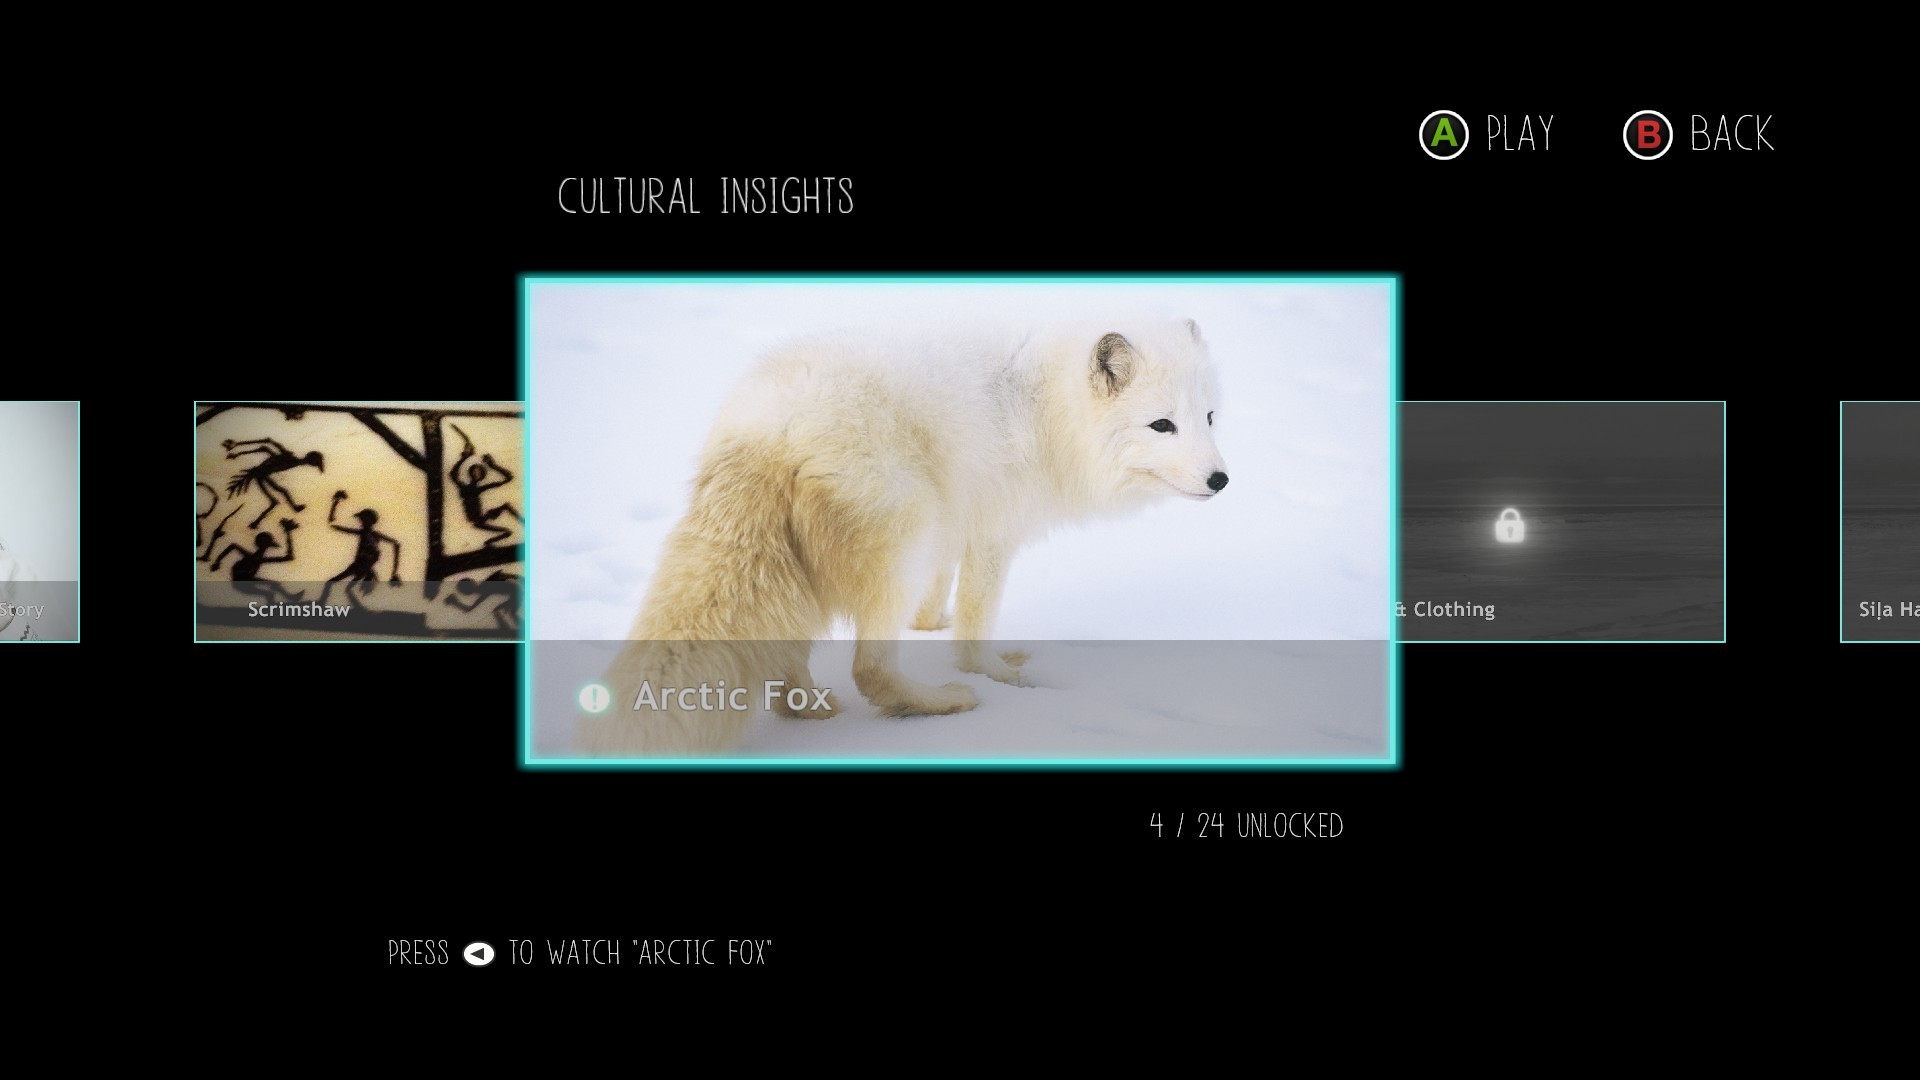
\includegraphics[scale=0.22]{images/statoarte/videona.jpg}}
\caption{Menù dei contenuti Serious di Never Alone.}
\label{fig:videona}
\end{figure}

Il gioco è stato sviluppato per PC, OS X, PlayStation3, PlayStation4, XboX360, XboxOne e Wii U. Come Valiant Hearts, anche Never Alone ha ricevuto ottime critiche, ed è stato premiato da ``Game for Changes'' come ``Most Impact'' e ``Game of the year''.


%--------------------------

\subsection{Super Mario}

Citiamo anche i giochi di Super Mario, in particolare modo riferendoci alle sue prime versioni (quindi titoli precedenti all'anno 1996, dove è comparso il primo Super Mario in 3D), in quanto sono state oggetto di studio riguardo le meccaniche platform 2D.

Ricordiamo che Super Mario è stato fra i primissimi giochi platform, cioè un gioco dove si salta da una piattaforma all'altra, spesso poste ad altezze diverse. Il gioco presenta anche una certa varietà di nemici, e le edizioni successive alla prima offrono anche un certo numero di ``power up'', cioè potenziamenti per l'avatar (per esempio la possibilità di sparare fiammelle dalla mano, in modo da uccidere i nemici anche da lontano e non per forza saltando loro addosso).
La principale difficoltà del gioco consiste nel coordinare salti e movimenti in base all'ambiente circostante, il giocatore mette quindi a dura prova i propri riflessi e tempismo durante il gameplay, il quale presenta una difficoltà di non poco superiore rispetto ai platform dei giorni nostri. I nemici presenti nel gioco sono vari, i più famosi sono i Goomba, i quali semplicemente vagano nel mondo, senza curarsi della presenza del player, altri nemici invece sono in grado di lanciare oggetti al giocatore, con lo scopo di ucciderlo.
E' stato particolarmente utile notare la gestione delle forze usate per il salto dell'avatar e di come quest'ultimo rimbalzi sopra i nemici dopo averli calpestati. La forza del salto, e quindi l'altezza massima raggiunta da Mario, è proporzionale alla durata della pressione del tasto A (usato appunto per saltare), quindi, brevi pressioni corrisponderanno a piccoli salti, lunghe pressioni invece produrranno il salto ad altezza massima. Inoltre, alcune versioni di Super Mario gestiscono anche la fase di atterraggio in base alla pressione del tasto A: in Super Mario World (1990)  per esempio, se la pressione del tasto continua anche dopo il raggiungimento del picco in altezza, la caduta risultava essere più lenta, non appena il tasto viene rilasciato si ha invece ha discesa rapida. Questo meccanismo è stato implementato per dare un maggior controllo al giocatore sulla precisione dei salti, in quanto meccanica fulcro del gameplay, la quale è spesso fondamentale per raggiungere punti particolari di gioco (come per esempio nemici in movimento).
In quasi tutti i Super Mario la gestione dei livelli gioco ha una struttura ad hub, cioè è presente una ``stanza centrale'' o mappa di riferimento, dalla quale accedere ai vari livelli.

\begin{figure}[h]
\centerline{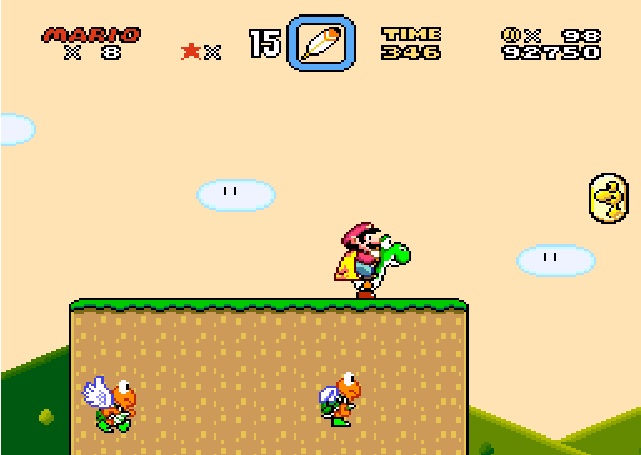
\includegraphics[scale=0.50]{images/statoarte/smwgameplay.jpg}}
\caption{Gameplay di Super Mario World.}
\label{fig:smwgameplay}
\end{figure}

Tutti i giochi di Super Mario sono disponibili per console Nintento. Negli ultimi anni, sono stati sviluppati dei titoli, sempre in 3D, ma con le vecchie meccaniche 2D, come per esempio ``New Super Mario Bros''.


%--------------------------

\subsection{Braid}

Braid è un gioco pubblicato nel 2008 e adotta delle meccaniche di gioco sia platform che puzzle. E' un gioco la cui meccanica predominante, oltre a quella dei salti, tipica dei platform, è quella di riportare indietro il tempo. Questo ``potere'', permette al giocatore di fare cose particolari fra cui risolvere indovinelli anche non banali. Durante l'evoluzione degli scenari, cambieranno anche gli elementi con cui potrà interagire il giocatore, (elementi come chiavi e relativa porta), e alcuni di questi reagiranno in modo particolare alla gestione del tempo, offrendo nuovi spunti per gli indovinelli proposti nel gioco. A differenza dei Super Mario, la potenza di salto non dipende dalla durata della pressione del relativo tasto, ma piuttosto ha una potenza standard. Anche qui i nemici possono essere uccisi tramite un salto sulla testa e questi uccidono il player per qualsiasi altro tipo di contatto. Ogni livello presenta un certo numero di collezionabili, i quali rappresentano i pezzi di un puzzle per un determinato ``mondo di gioco'', una volta raccolti tutti i pezzi sarà possibile ri-assemblare il puzzle e scoprire parte della storia principale. Come Super Mario, anche Braid ha una struttura dei livelli ad hub, il quale è rappresentato da una casa con delle stanze e porte al proprio interno, quindi ogni porta rappresenta l'accesso ad un mini mondo. In ogni stanza presente nella ``casa hub'' è presente un quadro raffigurante il puzzle da ricomporre coi pezzi raccolti nel mondo relativo a quella stanza.

I nemici presenti nel gioco sono in genere di 2 tipi:

\begin{itemize}
\item nemici stupidi: tendono a camminare in una direzione, e cambiare direzione nel caso si tocchi un muro (quindi nemici dalle caratteristiche simili ai Goomba di Super Mario);
\item nemici con carica: graficamente rappresentati con dei conigli, questi compaiono all'improvviso e dopo una breve carica, puntano il player con lo scopo di ucciderlo toccandolo.
\end{itemize}

\begin{figure}[h]
\centerline{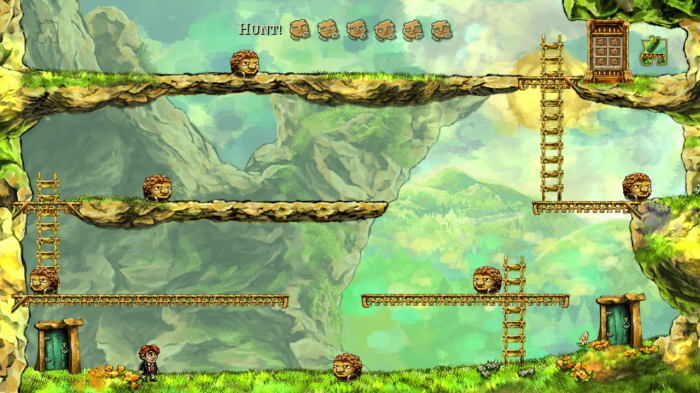
\includegraphics[scale=0.5]{images/statoarte/bgameplay.png}}
\caption{Gameplay di Braid.}
\label{fig:bgameplay}
\end{figure}

Il finale di gioco è sbloccato dopo che tutti i puzzle nei quadri sono stati riassemblati, a quel punto nella ``casa hub'' viene sbloccata una camera contenente il mondo finale.
Sono inoltre presenti nei vari livelli dei collezionabili segreti, i quali sono tutti molto difficili da notare. Se collezionati tutti, viene sbloccato un finale segreto alternativo.


%--------------------------

\subsection{The swapper}

The Swapper è un gioco puzzle-platform, rilasciato per varie piattaforme, fra cui Windows, Mac OS X, Linux e console come PlayStation3 e PlayStation4. Si tratta di un gioco fantascientifico, dove il giocatore si trova abbandonato su una nave spaziale di ricerca, e qui scopre uno strano device che gli permette di creare copie di se stesso e tele-trasportare la sua coscienza in uno dei suoi cloni. Questa meccanica, che consente al giocatore di proiettare in qualunque punto del gioco (tranne per punti specifici) cloni di se stesso, da una componente puzzle enorme al gioco, difatti, i livelli sono pieni di enigmi da risolvere tramite lo sdoppiamento del giocatore. Quasi tutti si basano sulla pressione di un bottone al giusto momento, e sul raccoglimento di vari oggetti sparsi per i livelli.

\begin{figure}[h]
\centerline{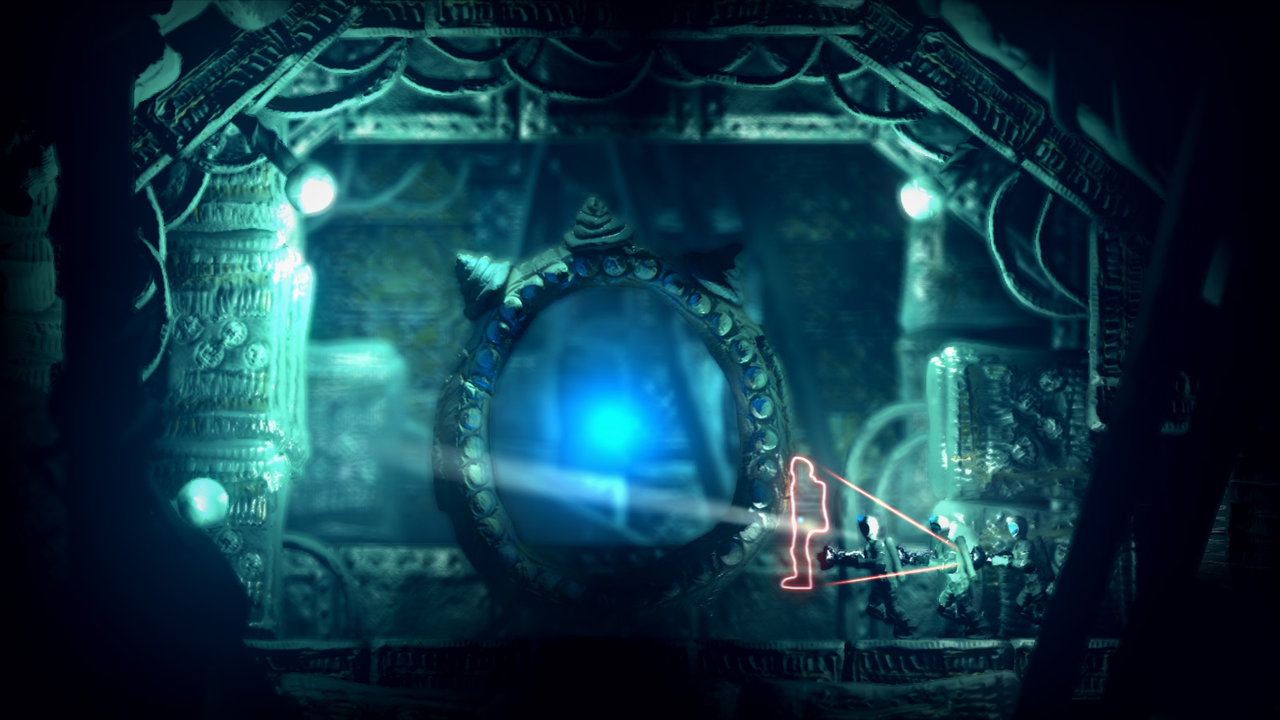
\includegraphics[scale=0.3]{images/statoarte/tsgameplay.png}}
\caption{Gameplay di The Swapper.}
\label{fig:pgameplay}
\end{figure}

%--------------------------

\subsection{Puppeteer}

Puppeteer è un gioco di tipo platform pubblicato nel 2013 per PlayStation3. Come si può notare in \myfig{\ref{fig:pgameplay}} sia la user interface che tutti i vari elementi di gioco, cercando di simulare uno spettacolo teatrale con dei burattini, difatti, è visibile il palcoscenico nella parte inferiore dello schermo e sono presenti anche i tendoni rossi sulle parti laterali e superiore. La narrazione, i dialoghi, i cambi di scena e tutti gli altri elementi richiamano benissimo le sensazioni che si provano durante uno spettacolo teatrale, il gioco risulta quindi essere un'opera molto artistica sotto questo punto di vista. Le meccaniche di gioco sono tante, in quanto, oltre al salto standard, sarà possibile fare un'azione speciale correlata al tipo di testa che si sta indossando, il cui numero si aggira intorno al centinaio (questo perché il personaggio ha perso la sua testa e la sostituisce con altre durante tutto il gioco). Ad un certo punto del gioco viene acquisito un altro potere, sottoforma di paio di forbici, le quali consentiranno di far arrampicare l'avatar su parti di mondo mentre queste vengono tagliate.

\begin{figure}[h]
\centerline{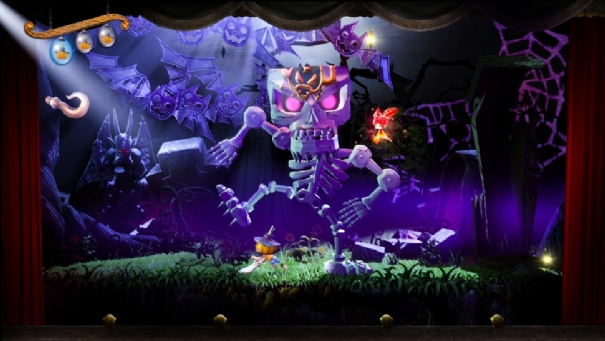
\includegraphics[scale=0.6]{images/statoarte/pgameplay.jpg}}
\caption{Gameplay di Puppeteer.}
\label{fig:pgameplay}
\end{figure}

Il gioco presenta una bassa difficoltà di superamento, difatti è un'opera adatta a tutti, soprattutto ad un pubblico infantile, il quale viene sicuramente affascinato da una grafica molto particolare che riesce decisamente a distinguersi dagli altri videogame, riuscendo a trasmettere al giocatore delle emozioni molto simili a quelle che darebbe un vero spettacolo di marionette.


%--------------------------

\section{Crescita dei Serious Game}

Esitono tanti altri Serious Game oltre a quelli citati finora (Valiant Hearts e Never Alone), e la loro diffusione è catalizzata da più fattori. 

Le ``Game Jam'' \cite{gamejamwiki} sono occasioni particolarmente efficaci per creare giochi del tutto innovativi. Questi sono degli eventi dalla durata media di 2-3 giorni che mettono assieme  persone dal diverso background, come game designer, sviluppatori, grafici e ogni altri tipo di figura interessata allo sviluppo dei videogame, al fine di creare dei giochi con una tematica in comune. Proprio fra il 2013-14 sono state organizzate delle Game Jam con tematiche Serious, grazie anche alla collaborazione con il progetto ``BOO-Games'' (progetto Europeo che mira alla sensibilizzazione riguardo lo sviluppo di Serious Game \cite{boogamesproject}\cite{boogamesprojecthome}). Una di queste Game Jam si è tenuta a Torino nel giugno del 2014 e ha avuto come tematica proprio l'informatica \cite{jamtoday}.

Un'altra comunità che sprona lo sviluppo dell'ambito Serious è ``Games for Change'' \cite{gamesforchange}, la quale organizza spesso eventi con talk di importanti figure del mondo videoludico per informare e sensibilizzare publisher, sviluppatori e insegnanti riguardo il potenziale dei Serious Game. Come già detto, è proprio ad eventi organizzati da "Games for Change" che giochi come Valiant Hearts e Never Alone hanno ricevuto importanti riconoscimenti.

Anche il Governo degli Stati Uniti d'America è attivo su questo fronte, e lo testimonia la scelta strategica di Barack Obama di investire milioni di dollari sull'ambito dell'education technology. Lo SBIR program (Small Business Innovation Research \cite{sbirprogram}) dell'istituto di Education Sciences darà più di un milione di dollari alle piccole aziende per la ricerca e lo sviluppo di prodotti commercializzabili per l'education technology. In reazione a ciò ci sono state varie proposte e sono nati giochi molto interessanti, come per esempio dei giochi riguardo le scienze naturali.


Adesso che abbiamo parlato dello stato dell'arte dei Serious Game e di altri giochi utili per i nostri studi, vediamo di affrontare meglio il nostro caso specifico.

\newpage

\chapter{Game Design}
\label{chap:game_design}

\section{Obiettivo}
\label{obiettivo}

L’obiettivo del lavoro di Tesi è stato quello di portare un pubblico che non conosce la tematica, ma è abituato a determinati contesti, che dimostra un interesse, anche non spiccato, verso questo bagaglio culturale, a mostrare curiosità nei confronti del tema del pre-Cinema.

Il pubblico a cui si fa riferimento è quello di ragazzi tra gli 11 ed i 18 anni, frequentanti perciò la scuola media inferiore e superiore. Con lo sviluppo, negli ultimi decenni, di differenti tipologie di media e di canali di informazione, tale fascia di età risulta estremamente abituata a contesti ludici o altre definizioni di intrattenimento sviluppate in forma digitale.
Ogni scelta di design è stata perciò effettuata tenendo conto del pubblico fruitore del prodotto finale, cercando perciò di limitare l’uso di metafore di gioco, o meccaniche che potessero risultare troppo complesse per un pubblico giovane.
Nonostante i ragazzi in tale fascia di età abbiano mostrato familiarità con il mezzo videoludico, abbiamo notato varie capacità di approccio per quanto riguarda l’input e l’interfacciamento con il prodotto sviluppato. Abbiamo quindi ritenuto opportuno tener conto anche delle differenti abilità di gioco ed abitudini ad utilizzare differenti dispositivi di input, e di conseguenza a prendere delle scelte di design che fossero state coerenti con quest’aspetto.

Risulta importante specificare che l’obiettivo primario del lavoro non è stato quello di insegnare o inculcare concetti ai ragazzi fruitori del gioco. Un approccio del genere avrebbe portato il prodotto ad essere caratterizzato da una forma didascalica e didattica, che avrebbe rischiato di sortire persino l’effetto opposto nei confronti degli utenti del gioco, l’essere noioso e poco divertente, poco appetibile ad un pubblico giovane.
Si è data perciò particolare importanza alla scelta di meccaniche di gioco divertenti, ambientazioni che avessero generato curiosità e stupore ed un gameplay stimolante. Elementi accompagnati dalla possibilità di fruire di schede informative e contenuti inerenti la tematica che si è deciso di affrontare.

\subsection{Piattaforma di riferimento e momenti museali}
\label{sec:piattaforma_di_riferimento}

Una scelta cruciale nella produzione di una qualsiasi forma di videogioco, è quella relativa alle piattaforme per cui sviluppare il prodotto finale. Risulta evidente come tale scelta influenzi pesantemente ogni elemento di design, dalla caratterizzazione più o meno dettagliata delle ambientazioni all’interfacciamento dell’utente.

Una prima analisi è stata quella relativa ai momenti museali a cui poter far riferimento. Per momenti museali intendiamo gli intervalli temporali in relazione all’entrata del pubblico in museo:
\begin{itemize}
	\item \textbf{Pre-visita.} Sono quei momenti in cui il pubblico si incuriosisce riguardo l’ambito museale e si interessa di una possibile visita. Volantini, passaparola, pubblicità, sono elementi che influenzano e caratterizzano il momento della pre-visita.
	\item \textbf{Visita.}  È l’intervallo temporale che il pubblico trascorre all’interno del museo, viene caratterizzato perciò dai contenuti veri e propri, oltre che da tutti gli altri elementi presenti all’interno del museo.
	\item \textbf{Post-visita.} Sono i momenti successivi alla visita del museo. Sono direttamente correlati alla soddisfazione provata dal pubblico, che può consigliare la visita ad altre persone, oltre che svolgere attività coerenti al contesto museale e provare interesse nei confronti di ciò che ha visitato.
\end{itemize}
Si è innanzitutto valutata la possibilità di sviluppare un prodotto fruibile all’interno del museo. L’applicazione avrebbe perciò avuto lo scopo di accompagnare la visita, tramite dei piccoli giochi, che avrebbero permesso di osservare alcuni degli elementi, presenti all’interno del museo, da prospettive diverse, generando nel pubblico una maggiore curiosità riguardo argomenti che sarebbero potuti risultare noiosi o poco interessanti. Un prodotto con un simile approccio è naturalmente sviluppabile per dispositivi mobili.

Secondo una nostra ipotesi, avvalorata anche da una personale ricerca di mercato, applicazioni del genere risultano molto interessanti per fasce di età inferiori rispetto a quella di riferimento per il progetto di Tesi.
I bambini, infatti, risultano particolarmente attratti da applicazioni semplici, immediate e veloci che possono rendere più piacevole la visita al museo, anche in compagnia di amici.
Ci si è quindi concentrati nei due restanti momenti museali, quelli precedenti e successivi alla visita.

Risulta importante specificare che la scelta della piattaforma di riferimento è stata effettuata anche in base alle meccaniche di gioco che si sono delineate durante le fasi di design del gameplay.
Abbiamo valutato la possibilità di sviluppare un casual game per dispositivi mobili, ma tale scelta avrebbe portato ad un prodotto superficiale, che sarebbe potuto risultare troppo semplicistico per il tema da voler affrontare.

\begin{figure}%[h]
	\centering
	% left bottom right top
	%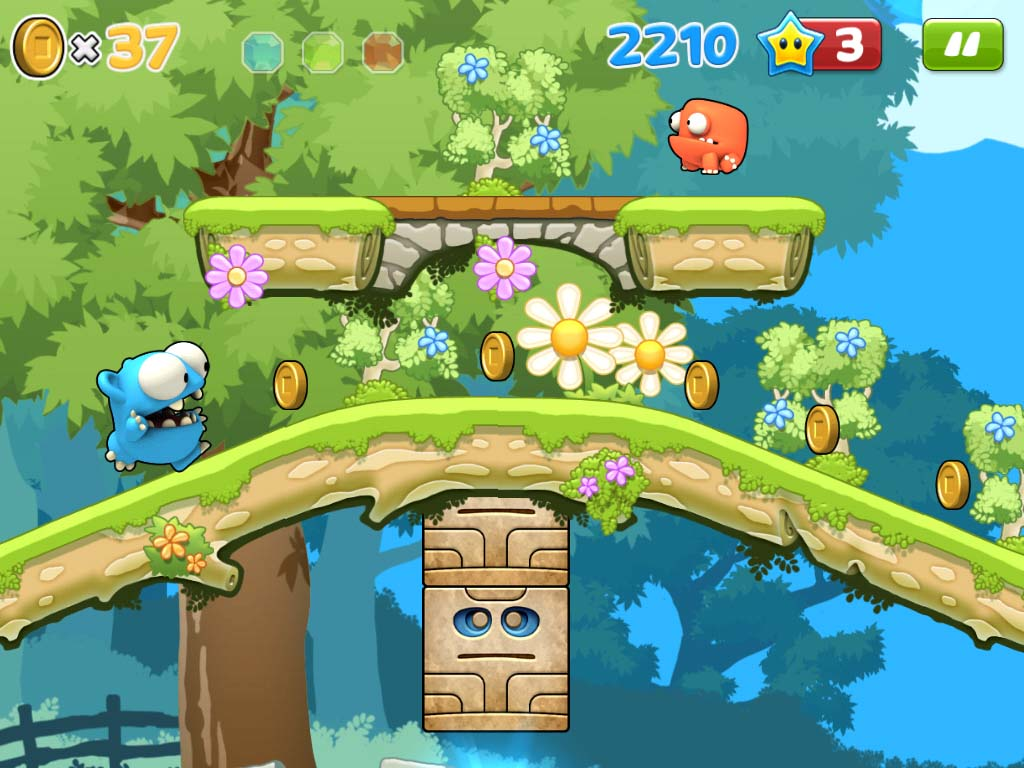
\includegraphics[clip= true, width= 0.8\columnwidth, trim= 1.5cm 3.0cm 0.6cm 0.0cm]{images/gameDesign/01_megarun.jpg}
	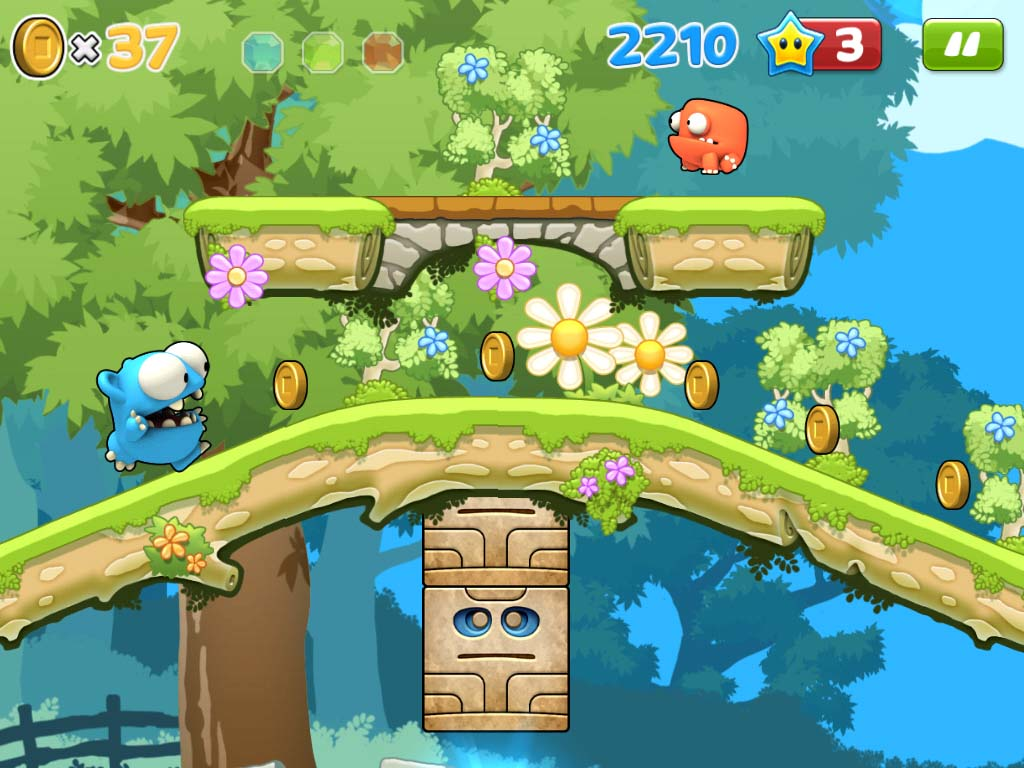
\includegraphics[width= 0.8\columnwidth]{images/gameDesign/01_megarun.jpg}
	\caption{Megarun: esempio di casual game.}
	\label{fig:casual_game}
\end{figure}

La natura platform/puzzle ideata durante le fasi di Design, ci ha spinto a sviluppare il prodotto per PC e console. Tali piattaforme permettono l’utilizzo di dispositivi di input più adatti alle tipologie di gameplay che sono state progettate, oltre che fornire una qualità visiva più consona all’estetica con cui si vuole caratterizzare il prodotto finito.
Tale scelta fornisce una ampia libertà di design, permettendo di sviluppare meccaniche complesse e profonde storyline, tipiche di una produzione di buon livello.

Concludendo, si è quindi scelto di sviluppare il videogioco per PC e console, con lo scopo di generare curiosità riguardo l’ambito del pre-cinema, attraverso meccaniche di gioco mirate, ambientazioni caratteristiche e schede informative studiate per fornire un buon supporto. Questo approccio risulta quindi coerente con i momenti museali di pre e post-visita, generando interesse nei confronti di un tema non ancora approfondito, o fornendo un buon metodo per osservare tematiche già note, apprese da una precedente visita, da un differente punto di vista.

\section{Meccaniche}
\label{sec:meccaniche}

Le meccaniche di gioco sono forse il nucleo più importante di una produzione videoludica di qualità, sono gli elementi che rimangono quando estetica, tecnologia e storia vengono meno, ed anche in queste condizioni, il prodotto, se caratterizzato da buone meccaniche, deve risultare piacevole ed efficace.
Il gameplay deve essere caratterizzato da regole semplici, ma allo stesso tempo flessibili, devono essere facili da capire, ma difficili da padroneggiare.

Il concetto di meccanica di gioco è strettamente legato a quello delle regole del game design, argomento che quindi non si limita ai videogiochi, ma a tutte le forme di intrattenimento che fanno riferimento al termine astratto di \textit{gioco}.
Abbiamo quindi fatto particolare attenzione al fornire al giocatore uno spazio di gioco in cui le meccaniche fornite avessero assicurato una sensazione di libertà, regolata però da limiti per circoscriverne le possibilità.
Il prodotto deve essere caratterizzato da pochi elementi di gameplay, ma che permettano al giocatore, entro certi limiti, di sentirsi libero di agire.

Ogni meccanica deve quindi essere semplice da capire e da utilizzare, ma deve richiedere un impegno ed uno studio progressivo per essere padroneggiata al meglio ed essere sfruttata in tutte le sue potenzialità.

Questo concetto è bene espresso nel libro \textit{The Art Of Game Design} \cite{artOfGameDesign}:
“Molti game designers sono d’accordo sul fatto che azioni interessanti che emergono col tempo siano la caratteristica di un buon gioco. Di conseguenza, il rapporto tra azioni significative e azioni di base è una buona misura di quanto un gioco emerga col tempo. Un gioco risulta elegante se permette al giocatore un piccolo numero di azioni di base, ma un grande numero di azioni significative.”

Chiaramente si tratta di un discorso soggettivo, ma ciò su cui abbiamo molto lavorato è stato trovare meccaniche di gioco semplici, ma che avessero permesso un vasto numero di possibilità in termini di level design e possibilità del giocatore.

\subsection{Elementi Platform}
\label{platform}
Il videogioco sviluppato presenta molte caratteristiche tipiche della categoria dei \textit{platform}.
Abbiamo scelto di utilizzare alcune meccaniche platform perché, oltre ad essere coerente con la rappresentazione che abbiamo deciso di creare durante le fasi di brainstorming, è un genere che sta tornando ad occupare una importante fetta di mercato. 

Il genere dei platform è nato nei primi anni ’80, ed ha avuto nel tempo una diffusione grandissima. Secondo wikipedia \cite{platform_wikipedia} , nel 1998 occupava il 15\% del mercato, nel 2006 ha avuto il suo massimo calo, arrivando ad occupare solo il 2\%, ma dal 2010 ha avuto una rinnovata popolarità, dovuta anche alla grande varietà degli endless runner che sono esplosi soprattutto nel mondo mobile. Anche la fervente attività degli sviluppatori indipendenti, sviluppatasi negli ultimi anni, ha fatto sì che il genere acquisisse di nuovo importanza nel settore. Tali studi, potendo contare su budget e mezzi limitati, hanno trovato, nel genere, un’importante base su cui poter costruire.

Per quanto riguarda il puro lato estetico, come mostrato in Figura~\ref{fig:platform_proportions}, il personaggio principale ha proporzioni non realistiche, molto accentuate in larghezza piuttosto che in altezza, con una proporzione che si avvicina all'1:1.

\begin{figure}%[h]
	\centering
	% left bottom right top
	%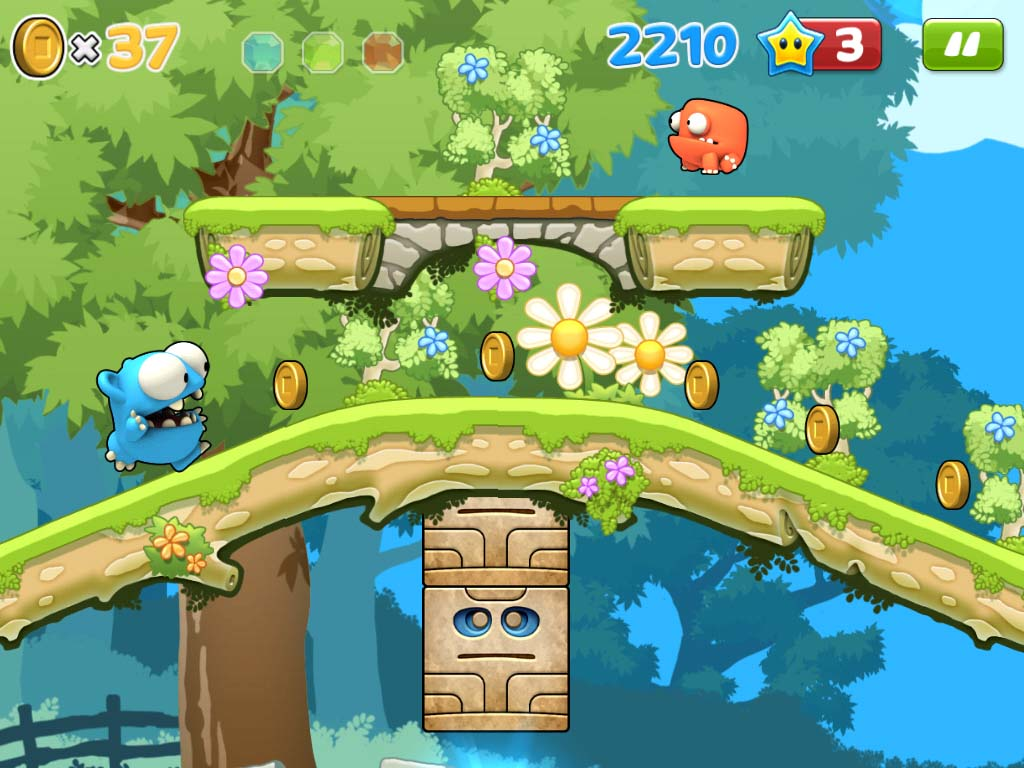
\includegraphics[clip= true, width= 0.8\columnwidth, trim= 1.5cm 3.0cm 0.6cm 0.0cm]{images/gameDesign/01_megarun.jpg}
	
\includegraphics[width= 0.9\columnwidth]{images/gameDesign/02_braid_SM.jpg}
	\caption{Proporzione del personaggio di un platform game: Braid e SuperMario.}
	\label{fig:platform_proportions}
\end{figure}

Caratteristici dei platform sono quegli elementi di gioco che richiedono soprattutto delle abilità di reazione e concentrazione del giocatore, come corsa, salto o usare piattaforme.

Per quanto riguarda il movimento del personaggio, abbiamo deciso di ricorrere ad una corsa bidirezionale, a velocità uniforme in entrambe le direzioni ed indipendente dalla pressione del tasto di riferimento o dell’inclinazione della levetta analogica del controller. Questo assicura un padroneggiamento più veloce della meccanica, che, per le caratteristiche di gioco, non richiede una eccessiva complessità.
La velocità massima di corsa è raggiunta in maniera non esattamente istantanea, questo per assicurarsi un movimento non troppo brusco e quindi poco intuitivo.

La bidirezionalità fa sì che il personaggio si giri nel caso venga indicato un movimento opposto rispetto all’attuale direzione. Questo permette di raggiungere di nuovo, dove permesso dal design dei livelli, posti già visitati in precedenza (Figura~\ref{fig:platform_corsa}). Tale scelta non deve essere presa in maniera superficiale, in quanto ci si deve assicurare che elementi di gioco, incontrati in differenti momenti della partita, non si interfaccino in maniera problematica tra di loro. 
\begin{figure}%[h]
	\centering
	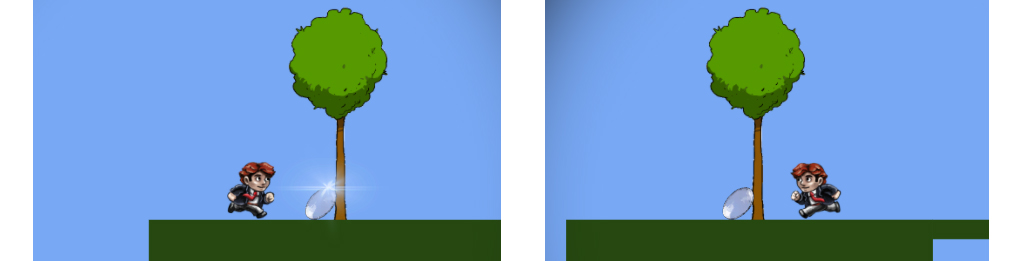
\includegraphics[width= \columnwidth]{images/gameDesign/03.jpg}
	\caption{Movimenti di corsa nel prototipo sviluppato}
	\label{fig:platform_corsa}
\end{figure}
In SuperMario Bros. (riferimento?) il personaggio può cambiare direzione, ma la camera non può tornare indietro, quindi, quando il personaggio arriva al bordo sinistro, è come se sbatta contro un muro invisibile.
La tipologia di gioco definita \textit{Endless Runner} invece, evita il problema impedendo al giocatore di invertire la direzione, nella maggior parte dei casi imponendo una corsa indipendente dall’input del giocatore o in altri casi semplicemente rallentabile o accelerabile (Figura~\ref{fig:platform_corsa_reali}).

\begin{figure}%[h]
	\centering
	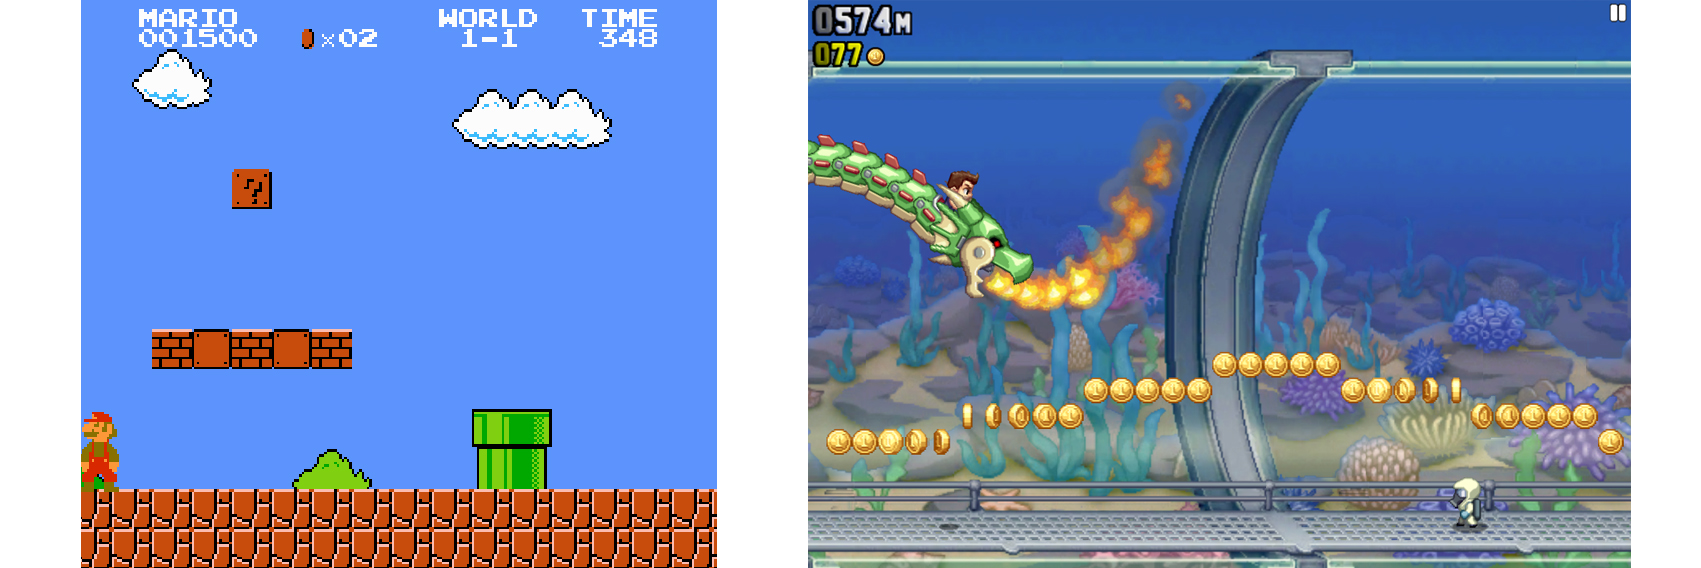
\includegraphics[width= \columnwidth]{images/gameDesign/04.jpg}
	\caption{Esempi di corsa: SuperMario e JetpackJoyride.}
	\label{fig:platform_corsa_reali}
\end{figure}

Per il salto, abbiamo deciso inizialmente di assegnare al personaggio una forza fissa verso l’alto, in seguito alla pressione del relativo bottone. Alcuni videogiochi invece assegnano una forza dipendente in maniera proporzionale dalla pressione del giocatore. Sono chiaramente due approcci differenti, il secondo fa sì che il salto sia una meccanica più complessa da padroneggiare, ma assicura delle possibilità di gameplay in più.
Durante i testing effettuati, abbiamo notato delle frequenti difficoltà nell’effettuare i salti, possiamo perciò pensare di prendere provvedimenti in tal senso, magari dando al giocatore un maggior controllo sulla potenza di salto, o limitando le sezioni in cui l’utilizzo del salto risulti troppo cruciale.

I movimenti del personaggio in aria sono controllabili attraverso i tasti direzionali. Perciò, dopo il salto o in seguito ad una caduta, il giocatore può direzionare o aggiustare la traiettoria di discesa. Non tutti i videogiochi platform assicurano tale comportamento, ma abbiamo ritenuto potesse essere utile per non frustrare eccessivamente il giocatore in seguito ad un salto non perfettamente calibrato al momento dello stacco.
La caduta del personaggio è soggetta ad una gravità 3 volte superiore al normale, è un elemento già presente in \textit{SuperMario} e ampiamente utilizzato nei giochi del genere per garantire una sensazione di repentinità al giocatore. La velocità di caduta è comunque limitata per garantirne il controllo.

\begin{figure}%[h]
	\centering
	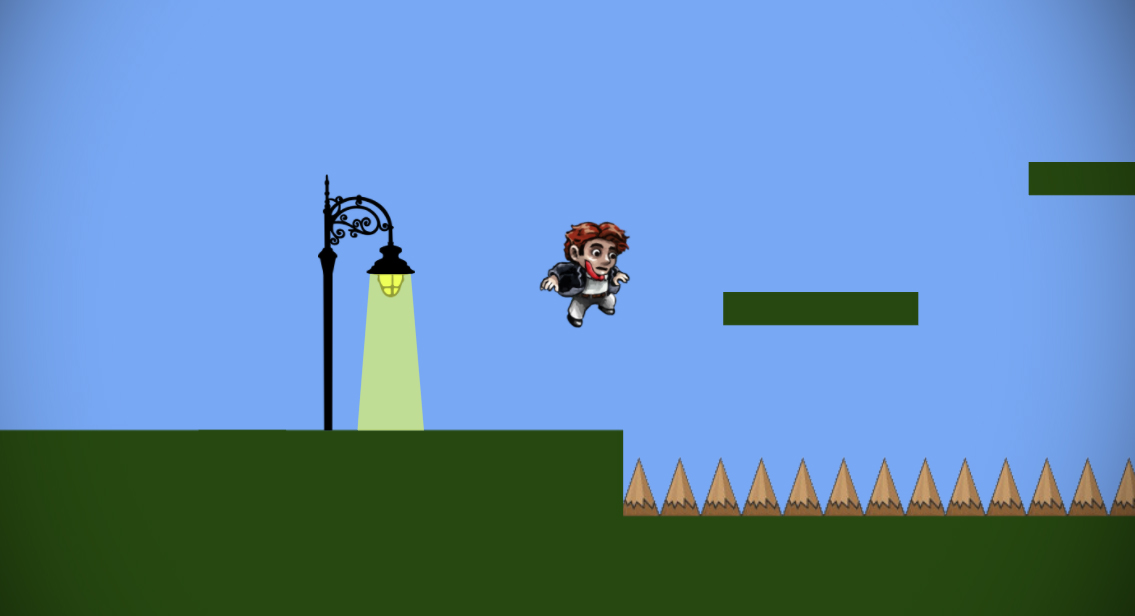
\includegraphics[width= 0.8\columnwidth]{images/gameDesign/05.jpg}
	\caption{Personaggio del prototipo, durante un salto.}
	\label{fig:platform_salto}
\end{figure}

Oltre alle meccaniche di corsa e salto, abbiamo dato la possibilità al personaggio di salire e scendere le scale. Questa è una meccanica non essenziale, che non aggiunge possibilità rispetto a quelle che non possa garantire una serie di salti, ma garantisce una maggiore sensazione di libertà al giocatore e permette una maggiore pulizia per quanto riguarda il level design. Le scale infatti, come mostrato in Figura~\ref{fig:platform_scala_piattaforme}, consentono di raggiungere luoghi per cui, altrimenti sarebbero state necessarie numerose piattaforme, che avrebbero potuto rendere la realizzazione dei livelli molto difficoltosa e confusa.

\begin{figure}%[h]
	\centering
	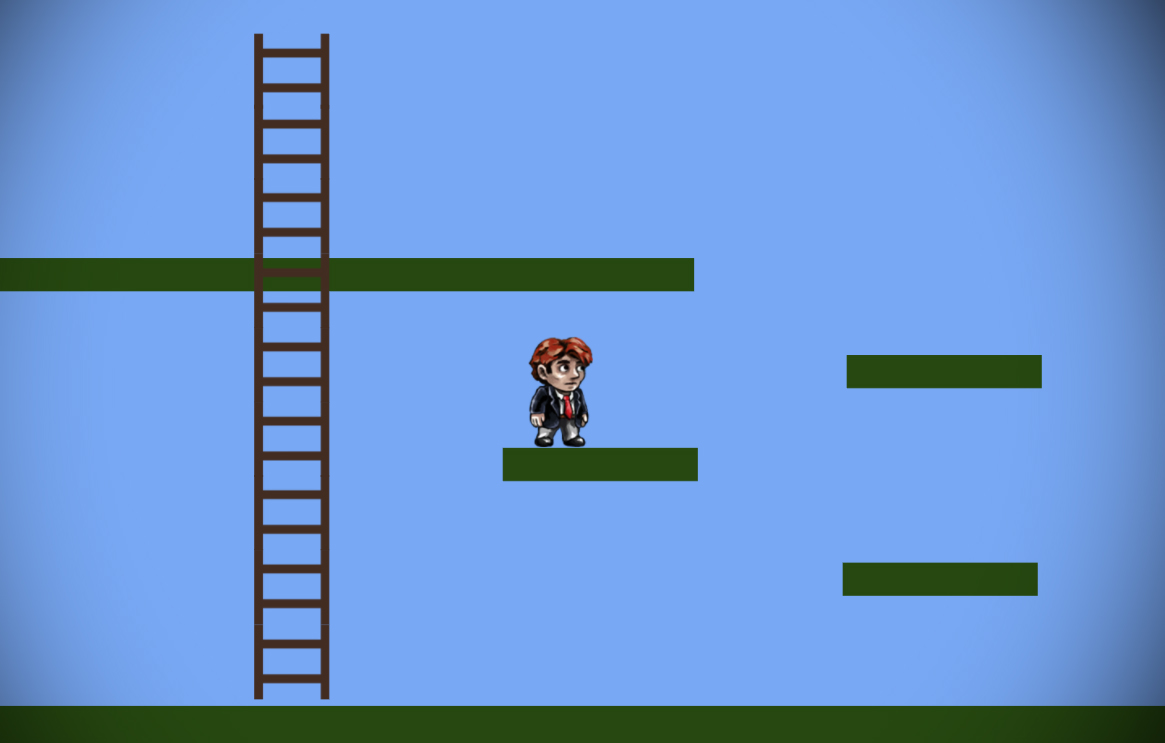
\includegraphics[width= 0.8\columnwidth]{images/gameDesign/06.jpg}
	\caption{Confronto tra utilizzo di scale e piattaforme equivalenti.}
	\label{fig:platform_scala_piattaforme}
\end{figure}

Le meccaniche di salto, controllo del personaggio in aria ed utilizzo scale sono state ispirate dal videogioco Braid (riferimento?), anche qui infatti il salto fornisce una forza indipendente dalla pressione del tasto e la possibilità di controllare il personaggio in caduta è una meccanica importante di gioco, anche se, rispetto a Braid, la forza impressa dal salto risulta meno forte e la gravità in caduta più espressiva, i movimenti in Braid appaiono più naturali, nel nostro caso invece più repentini ed eccessivi.

Sono state incluse nel gioco anche delle piattaforme mobili (Figura~\ref{fig:platform_piattaforme_mobili}). Queste hanno un movimento lineare tra due punti, uno dei quali raggiungibile dal personaggio, mentre l’altro si pone come obiettivo finale del movimento. Sono un elemento che mette alla prova le abilità di tempismo e di concentrazione del giocatore. Tali piattaforme risultano attraversabili dal basso verso l’alto, questo per permettere una maggiore libertà di approccio all’utente.
Durante i test effettuati, abbiamo notato che, spesso, i giocatori fanno fatica a comprendere i momenti esatti in cui la piattaforma cambia di direzione. Si sta perciò valutando se, nel prodotto finale non possa essere utile introdurre degli elementi che, graficamente, rappresentino dei limiti di inizio e fine corsa.

\begin{figure}%[h]
	\centering
	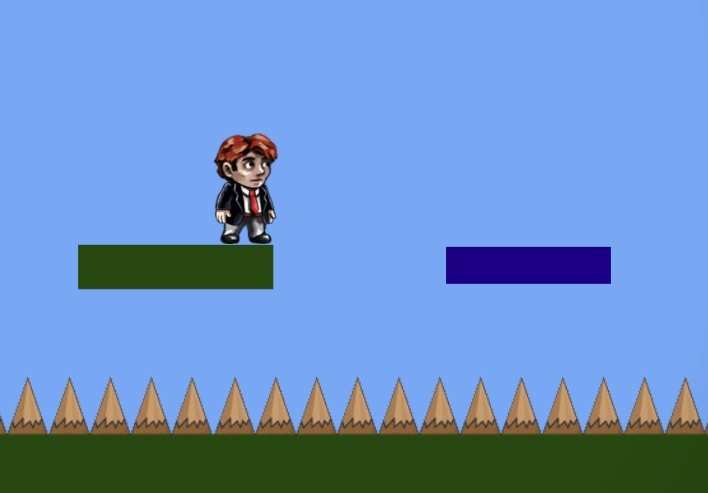
\includegraphics[width= 0.6\columnwidth]{images/gameDesign/07.jpg}
	\caption{Esempio di piattaforme mobili sviluppate.}
	\label{fig:platform_piattaforme_mobili}
\end{figure}

Graficamente, abbiamo deciso di rappresentare il terreno normale con una colorazione verde. Tale elemento non è attraversabile in nessuna direzione. Il personaggio collide sempre con esso.

Le piattaforme mobili vengono invece rappresentate con una colorazione blu scura, come si può osservare in Figura~\ref{fig:platform_piattaforme_mobili}.

Un altro terreno, che abbiamo deciso di sviluppare, permette di essere attraversato in entrambe le direzioni, ma solo se il personaggio sta utilizzando una scala. Permette appunto di attraversare terreni normalmente non attraversabili, ma caratterizzati dalla presenza della scala. La colorazione per questo tipo di terreno rimane comunque quella verde. Abbiamo verificato, tramite test e prototipazione, che questa scelta non influisce sulla comprensibilità della meccanica, in quanto caratterizzata dalla presenza della scala.

Parallelamente abbiamo ritenuto necessario sviluppare una tipologia differente di terreno, che permette di essere superato dal basso, ad esempio con un salto del personaggio. Non è attraversabile dall’alto. Tale scelta apre la strada ad una nuova meccanica, in quanto realizza una via a “senso unico” che può essere utile in fase di level design. Questo terreno invece, è differenziato dal resto tramite una colorazione blu più tenue rispetto alle piattaforme mobili.

Le 3 tipologie di terreno possono essere osservate in Figura~\ref{fig:platform_terreni}.

\begin{figure}%[h]
	\centering
	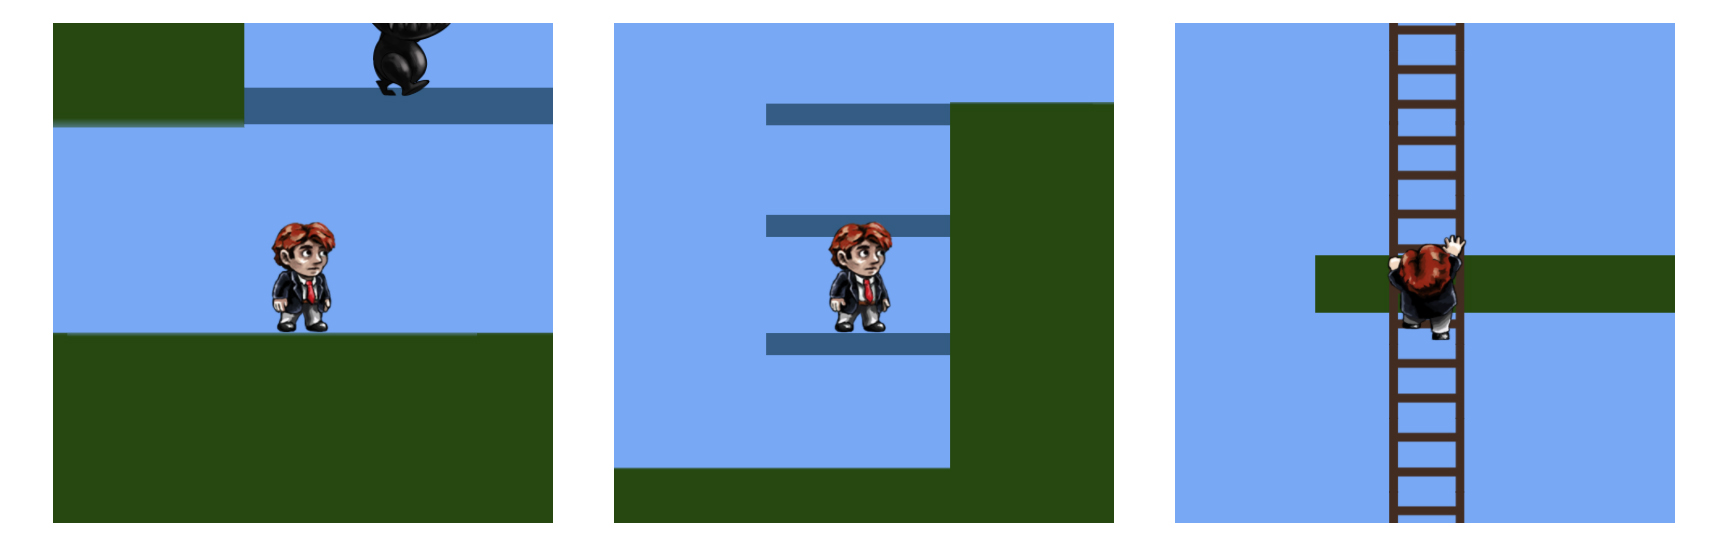
\includegraphics[width= \columnwidth]{images/gameDesign/08.jpg}
	\caption{Esempi delle tre tipologie di terreno sviluppate.}
	\label{fig:platform_terreni}
\end{figure}

\subsection{Elementi Puzzle}
\label{elementi_puzzle}

Oltre alle meccaniche Platform, che richiedono soprattutto reattività, tempismo e concentrazione del giocatore, il videogioco presenta anche caratteristiche tipiche del genere dei \textit{Puzzle Games}.

Questa categoria di videogiochi enfatizza soprattutto la risoluzione di enigmi e puzzles. Il giocatore deve perciò possedere le capacità di osservare la situazione in cui si trova il personaggio, analizzarne gli elementi, e capire in che modo debbano essere sfruttati ed usati per superare una determinata sezione o raggiungere un obiettivo.
Sono perciò richieste quelle che il libro \textit{The Art Of Game Design}\cite{artOfGameDesign} Definisce come abilità mentali (\textit{Mental Skills}):
“Le abilità mentali includono le capacità di memoria, osservazione e risoluzione di puzzle. Sebbene alcune persone evitino giochi che richiedono troppo impegno per quanto riguarda queste capacità, è raro che i giochi non le includano anche in piccola parte, perché i giochi sono interessanti quando ci sono decisioni interessanti da prendere, e prendere decisioni è una abilità mentale.”

Risulta necessario specificare che, nella fase di Level Design, abbiamo fatto particolare attenzione nel mescolare intelligentemente elementi platform e puzzle, in modo da essere in sintonia tra loro, senza che uno dei due elementi apparisse predominante sull’altro e che l’esperienza non risultasse eccessivamente frenetica e frustrante da un lato o lenta e noiosa dall’altro.
Le dinamiche puzzle ci hanno permesso anche di fare design riguardo il possibile utilizzo di strumenti particolari del pre-Cinema in maniera originale e curiosa (riferimento al capitolo), inserendo quindi elementi di gioco non presenti in altri esponenti del settore.
Elementi classici del puzzle game, che abbiamo inserito sono, ad esempio, leve, pulsanti, casse, porte, bilance e sequenze di bottoni.

Le leve (Figura~\ref{fig:platform_leve}) sono utilizzate per avere un effetto diretto sullo scenario di gioco. Generalmente, le abbiamo utilizzate per spostare elementi dell’ambientazione o attivare meccanismi.

\begin{figure}%[h]
	\centering
	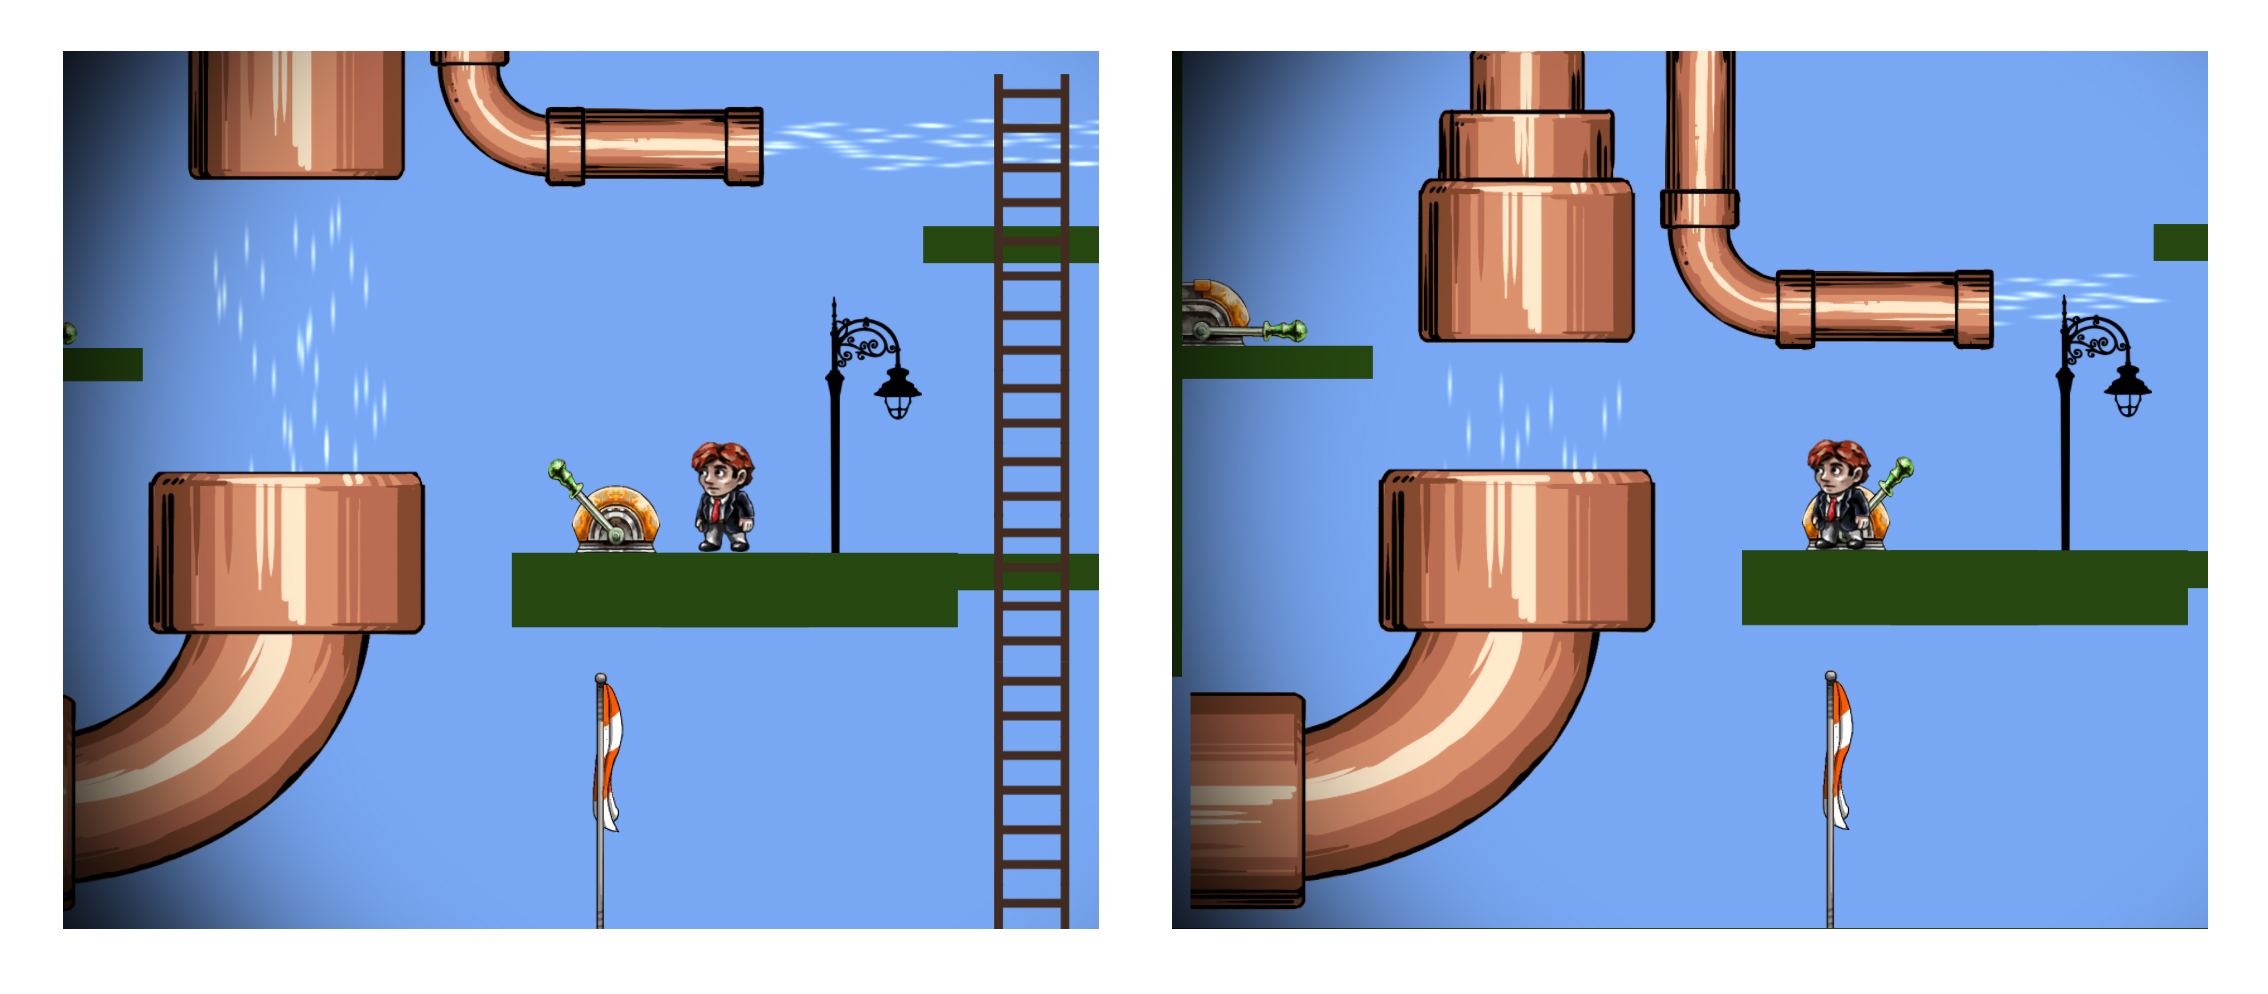
\includegraphics[width= \columnwidth]{images/gameDesign/09.jpg}
	\caption{Esempio di leva. Utilizzata per interagire con un elemento dello scenario.}
	\label{fig:platform_leve}
\end{figure}

I pulsanti a pressione possono essere intesi, concettualmente, come le leve, hanno un effetto immediato su alcuni elementi dello scenario. Nel nostro caso in particolare, abbiamo preferito associarli ad aperture e chiusure di porte, portoni o elementi traslabili che impediscono o permettono il passaggio del personaggio da una zona all’altra di gioco. Questa scelta è stata fatta per permettere al giocatore di capire immediatamente l’effetto di un bottone, spesso anche prima di premerlo.

L’attivazione dei bottoni avviene nel momento in cui il personaggio sale su di essi, hanno perciò un funzionamento a pressione. L’effetto diretto avviene al momento dell’attivazione. Quando il personaggio scende, i bottoni possono disattivarsi e quindi invertire l’effetto sortito sullo scenario di gioco o rimanere attivi e mantenere l’effetto nel tempo. Tale scelta dipende dal particolare utilizzo e quindi da scelte di level design.

I bottoni, come già specificato, vengono attivati dalla pressione su di essi, sia che venga applicata dal personaggio principale, che da un nemico (riferimento al capitolo). Come mostrato in Figura~\ref{fig:platform_bottoni} abbiamo comunque ritenuto utile inserire delle casse come elemento di gioco. Esse permettono di premere i bottoni senza la presenza del personaggio, oltre che salirci sopra per raggiungere posti più elevati.

\begin{figure}%[h]
	\centering
	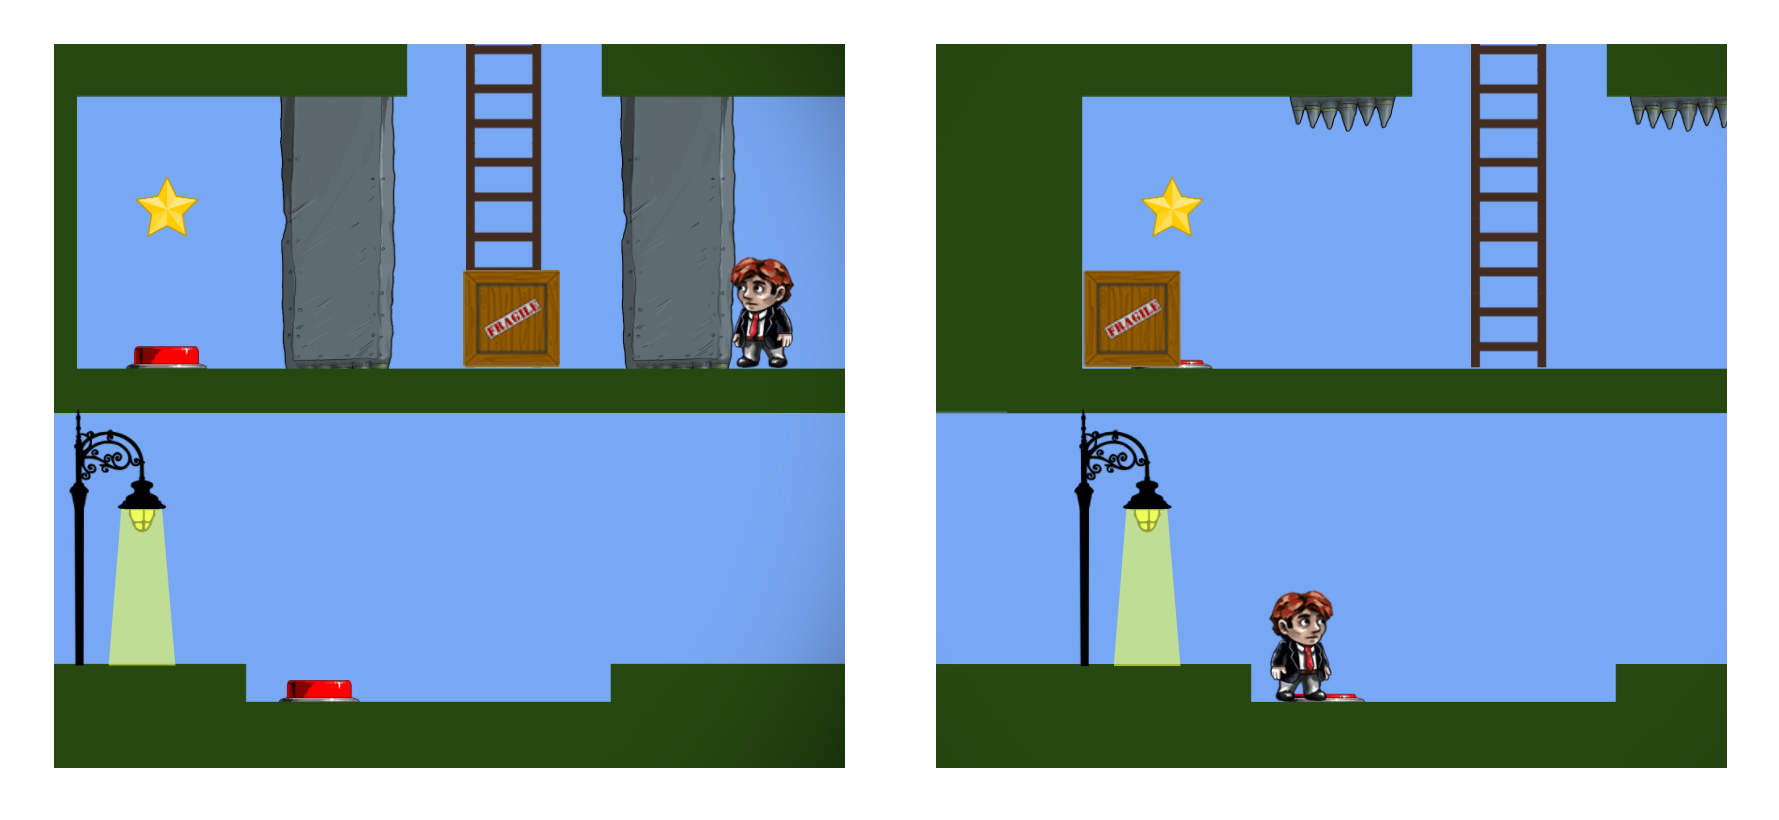
\includegraphics[width= \columnwidth]{images/gameDesign/10.jpg}
	\caption{Bottoni premuti dal personaggio e da una cassa.}
	\label{fig:platform_bottoni}
\end{figure}

Coerentemente con il concetto di pressione e pesi, abbiamo introdotto nel gioco anche delle bilance (Figura~\ref{fig:platform_bilancia}). Per semplicità, abbiamo ipotizzato che ogni elemento di gioco abbia una massa, relativamente alla bilancia, di una unità. Ipotizzando perciò che in un piatto ci sia una cassa, per avere una situazione di equilibro, è sufficiente che sull’altro piatto ci sia il personaggio. La bilancia, come le leve, permette di attivare un elemento dello scenario. È stata utilizzata, ad esempio, per un enigma in cui è necessario spostare un numero di nemici sufficienti in un piatto, per far sì che l’altro si alzi e attivi un bottone.

\begin{figure}%[h]
	\centering
	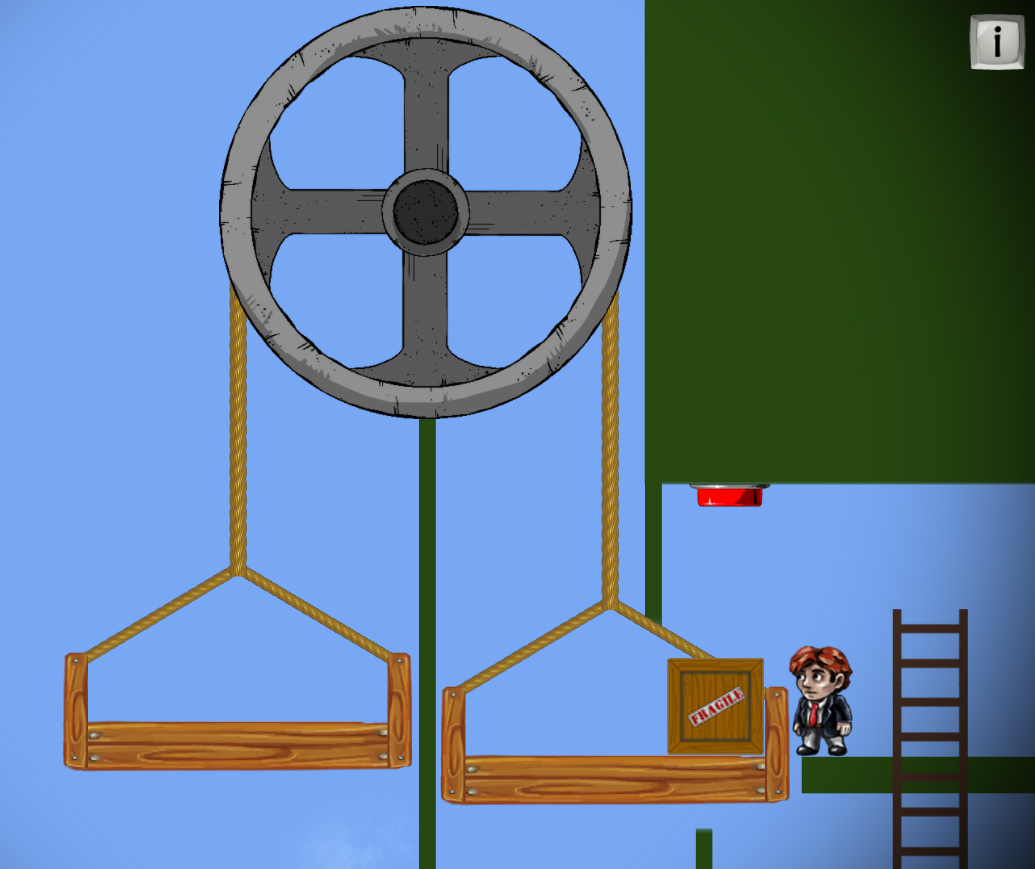
\includegraphics[width= 0.5\columnwidth]{images/gameDesign/11.jpg}
	\caption{Bilancia.}
	\label{fig:platform_bilancia}
\end{figure}

Un altro elemento interessante sono le sequenze di bottoni (Figura~\ref{fig:platform_sequenza_bottoni}
). Queste hanno lo stesso funzionamento dei bottoni singoli ma, per interagire con una porta è necessario attivarli tutti nella giusta sequenza. Se il primo bottone premuto è quello giusto, questo rimane attivo, se il secondo non è giusto, vengono disattivati tutti e la sequenza deve ricominciare dall’inizio. Quando vengono premuti tutti i bottoni nella giusta sequenza, viene attivato l’elemento dello scenario prestabilito, nel nostro caso le sequenze di bottoni sono sempre state utilizzate per aprire porte.

\begin{figure}%[h]
	\centering
	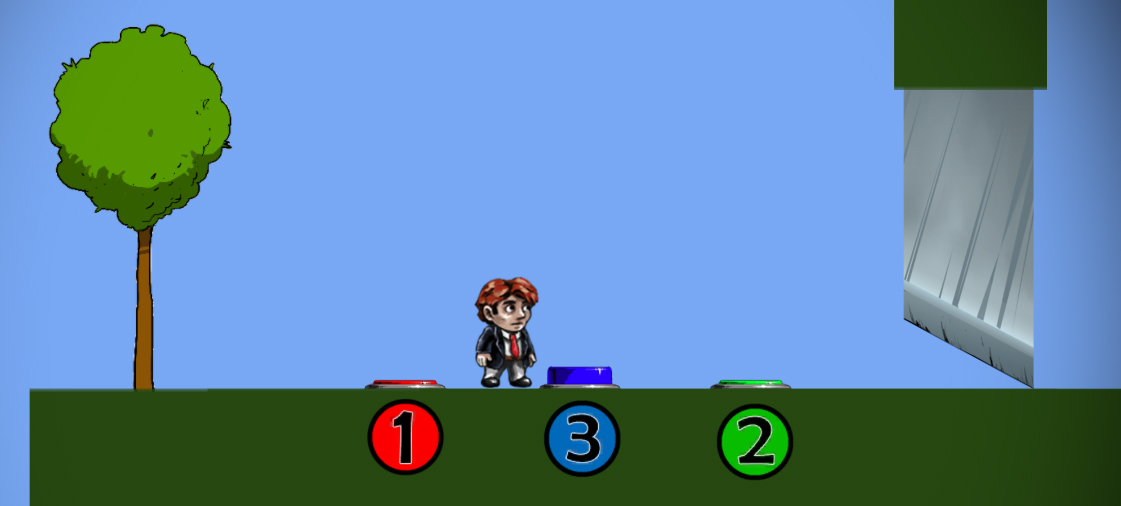
\includegraphics[width= 0.7\columnwidth]{images/gameDesign/12.jpg}
	\caption{Sequenza di bottoni.}
	\label{fig:platform_sequenza_bottoni}
\end{figure}

Viene riportata di seguito l’analisi di un enigma presente in uno dei livelli sviluppati. Nella figura \ref{fig:platform_enigma} si possono notare alcuni elementi non ancora analizzati, come il nemico, la lanterna magica o la stella, fare riferimento ai relativi capitoli (riferimenti) per approfondimenti sul loro utilizzo, che qui verrà spiegato in maniera superficiale.

\begin{figure}%[h]
	\centering
	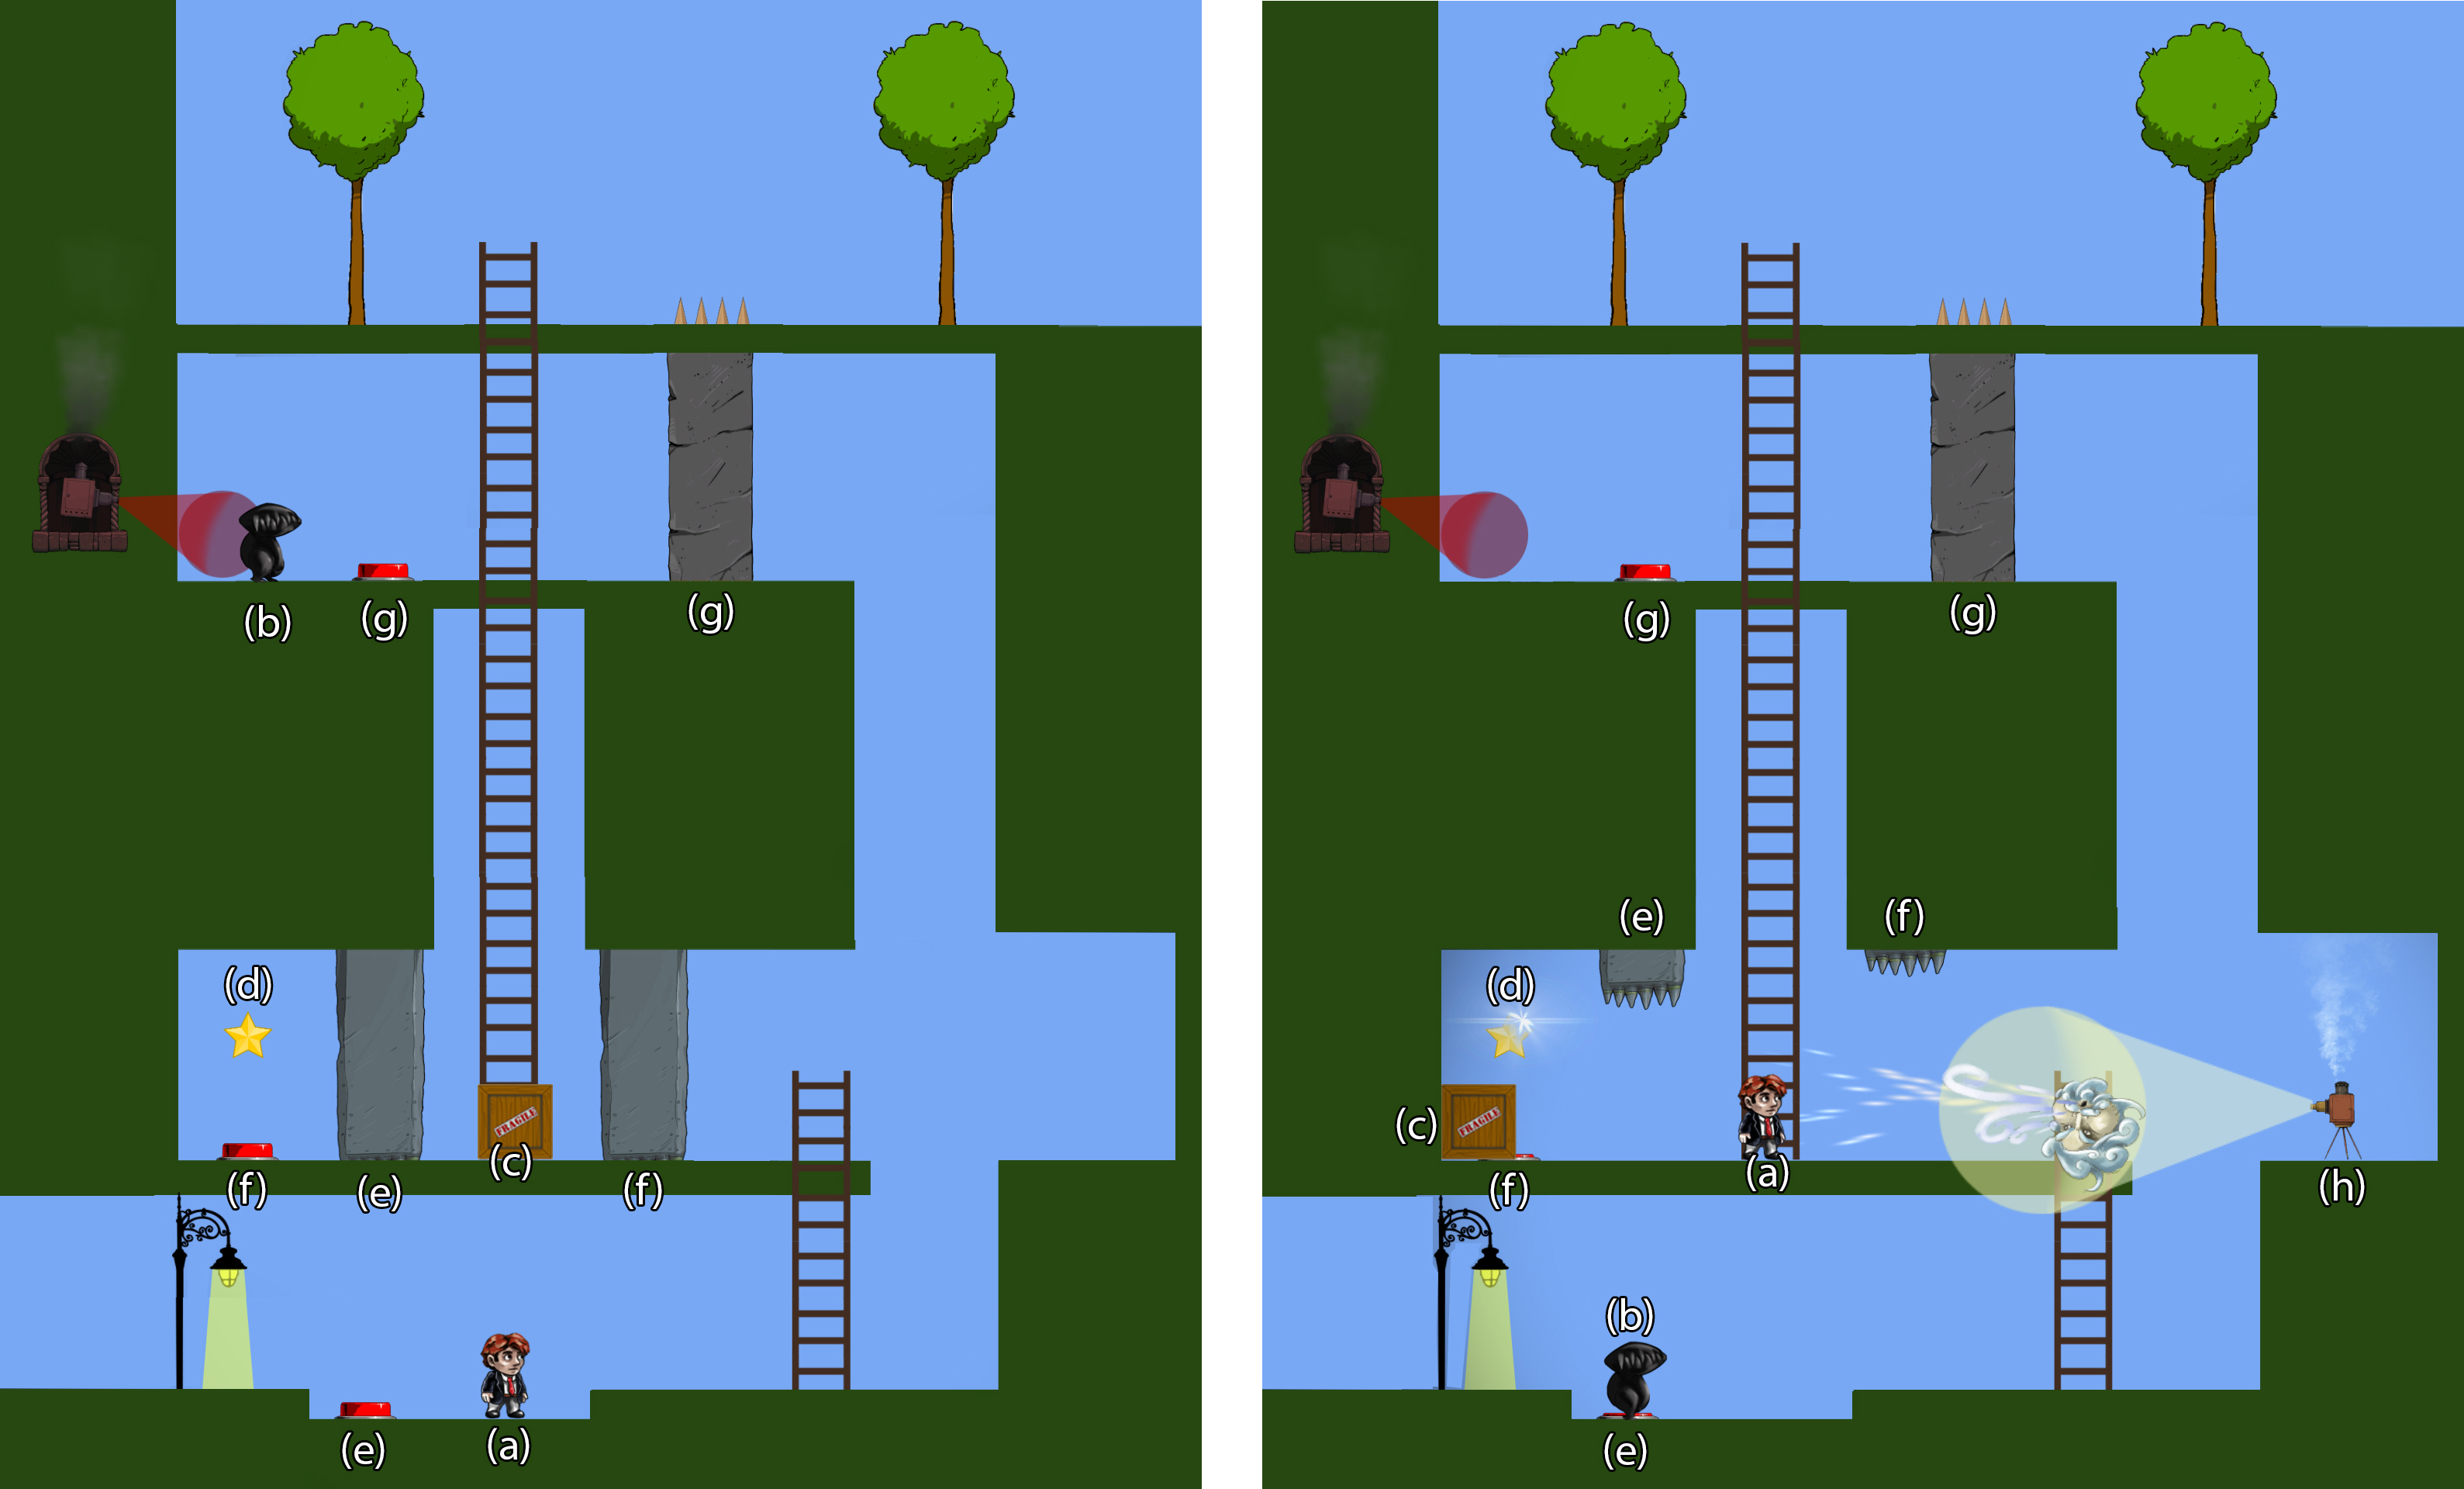
\includegraphics[width= \columnwidth]{images/gameDesign/13.jpg}
	\caption{Esempio di enigma.}
	\label{fig:platform_enigma}
\end{figure}

Come spesso avviene nei vari livelli sviluppati, la via per proseguire non richiede la completa risoluzione dell’enigma, ma solo la parte più semplice di esso, così da permettere, anche ai giocatori non interessati al raccoglimento di tutti i collezionabili, di proseguire con la partita.
In figura~\ref{fig:platform_enigma} vengono contrassegnati con la stessa lettera i bottoni e le relative porte che vengono azionate.

Il personaggio può subito porsi sopra il bottone “e” e notare l’apertura della relativa porta, che conduce ad una stanza con un altro bottone. Il giocatore capisce che la pressione di questo bottone è l’unico modo per proseguire. Raggiunge perciò un luogo favorevole per piazzare a terra la lanterna magica e sfruttarne il vento prodotto per spingere la cassa, bloccata però dalla porta “e”. Il personaggio deve quindi tornare sul bottone “e” e permettere alla cassa di premere il bottone “f”. Il personaggio può quindi raggiungere le scale e salire. Il nemico, premendo il pulsante “g”, attiva una porta con degli spuntoni, che blocca il raggiungimento dell’uscita, posta nella zona in alto a destra dell’immagine. Si deve perciò fare attenzione ad avere il giusto tempismo.

Come si può notare dall’immagine, il personaggio principale può quindi raggiungere l’uscita, ma rimane una stella da raccogliere. Come già specificato, solo la parte obbligatoria dell’enigma è stata risolta, ma non quella opzionale per il raccoglimento della stella.

Il giocatore può quindi, una volta salita la scala ed arrivati sul livello del nemico, scendere dalla scala, aspettare che il nemico si volti verso la porta/macigno, saltare il nemico, premere il bottone “b” e permettere così al nemico di cadere al piano inferiore. Questo, camminando, raggiungerà la zona con il bottone “e”, senza la possibilità di uscirne. Continuerà perciò ad attivare la porta che conduce alla stanza con la stella, che potrà quindi essere agilmente raccolta dal personaggio. Una volta collezionata, si può proseguire lungo il livello.
La seconda immagine in Figura~\ref{fig:platform_enigma} mostra l’enigma completamente risolto.

\subsection{Camera e Puntatore}
\label{sec:camera_e_puntatore}

Per quando riguarda la camera, abbiamo fatto in modo che questa fosse sempre approssimativamente centrata sul personaggio principale. In realtà usa una funzione che ne ammorbidisce il movimento, non segue perciò perfettamente il personaggio, ma tende in breve tempo alla sua posizione. Questa scelta è stata presa per rendere l’effetto meno brusco e quindi più gradevole alla vista.
Abbiamo anche ritenuto necessario includere la possibilità di evitare che la camera inquadri porzioni di scena non previste. È stata perciò valutata la capacità di gestire dei limiti della scena. Questa opzione è stata utilizzata solamente nel livello centrale, che funge da accesso agli altri livelli, ma sicuramente può fornire un mezzo ulteriore, in fase di design di altre meccaniche.

In seguito al design della meccanica di gioco principale, quella della Lanterna Magica (Riferimento), si è valutata la possibilità di inserire, per non confondere eccessivamente il giocatore, la possibilità di utilizzare un puntatore anche nelle normali fasi di gioco.

\begin{figure}%[h]
	\centering
	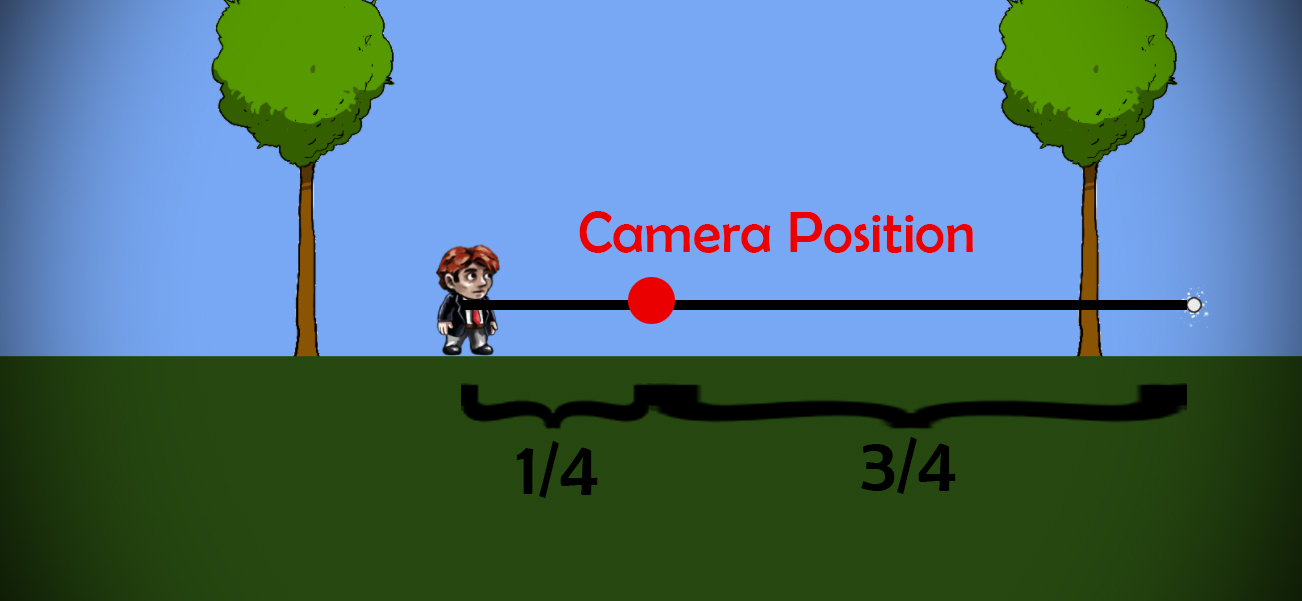
\includegraphics[width= 0.85\columnwidth]{images/gameDesign/15.jpg}
	\caption{Spostamento della camera in relazione alla posizione del personaggio e del puntatore.}
	\label{fig:camera_posizione_1_4}
\end{figure}

Il puntatore permette all’utente di spostare la camera dal personaggio principale ed osservare quindi porzioni di gioco che, normalmente, non sarebbero presenti nella visuale standard.
Il design del puntatore è stato un passaggio particolarmente difficile, che abbiamo perfezionato col tempo, in seguito allo sviluppo e test di vari prototipi.
Una delle prime versioni che abbiamo sviluppato, faceva tendere la posizione della camera al punto posto ad 1/4 del segmento che congiungeva il personaggio ed il puntatore, questo permetteva un allontanamento della camera dal personaggio, così da poter inquadrare una porzione di schermo maggiore (Figura~\ref{fig:camera_posizione_1_4}).

Ci siamo però resi conto che, nonostante l’effetto risultante fosse gradevole, l’utilità era particolarmente ridotta, in quanto non era possibile inquadrare elementi particolarmente lontani.
Si è perciò ipotizzato di allontanare la camera, lungo l’asse perpendicolare allo schermo, progressivamente con l’allontanarsi del puntatore dal personaggio.
In questo modo si è riusciti, con un effetto visivo di ridimensionamento degli elementi a schermo, ad inquadrare una porzione più grande di scena. Il maggiore problema riscontrato era comunque quello di un effetto forse troppo “pesante” all’occhio umano, che avrebbe perciò potuto generare confusione o addirittura fastidio al giocatore (Figura~\ref{fig:camera_allontanamento}).

\begin{figure}%[h]
	\centering
	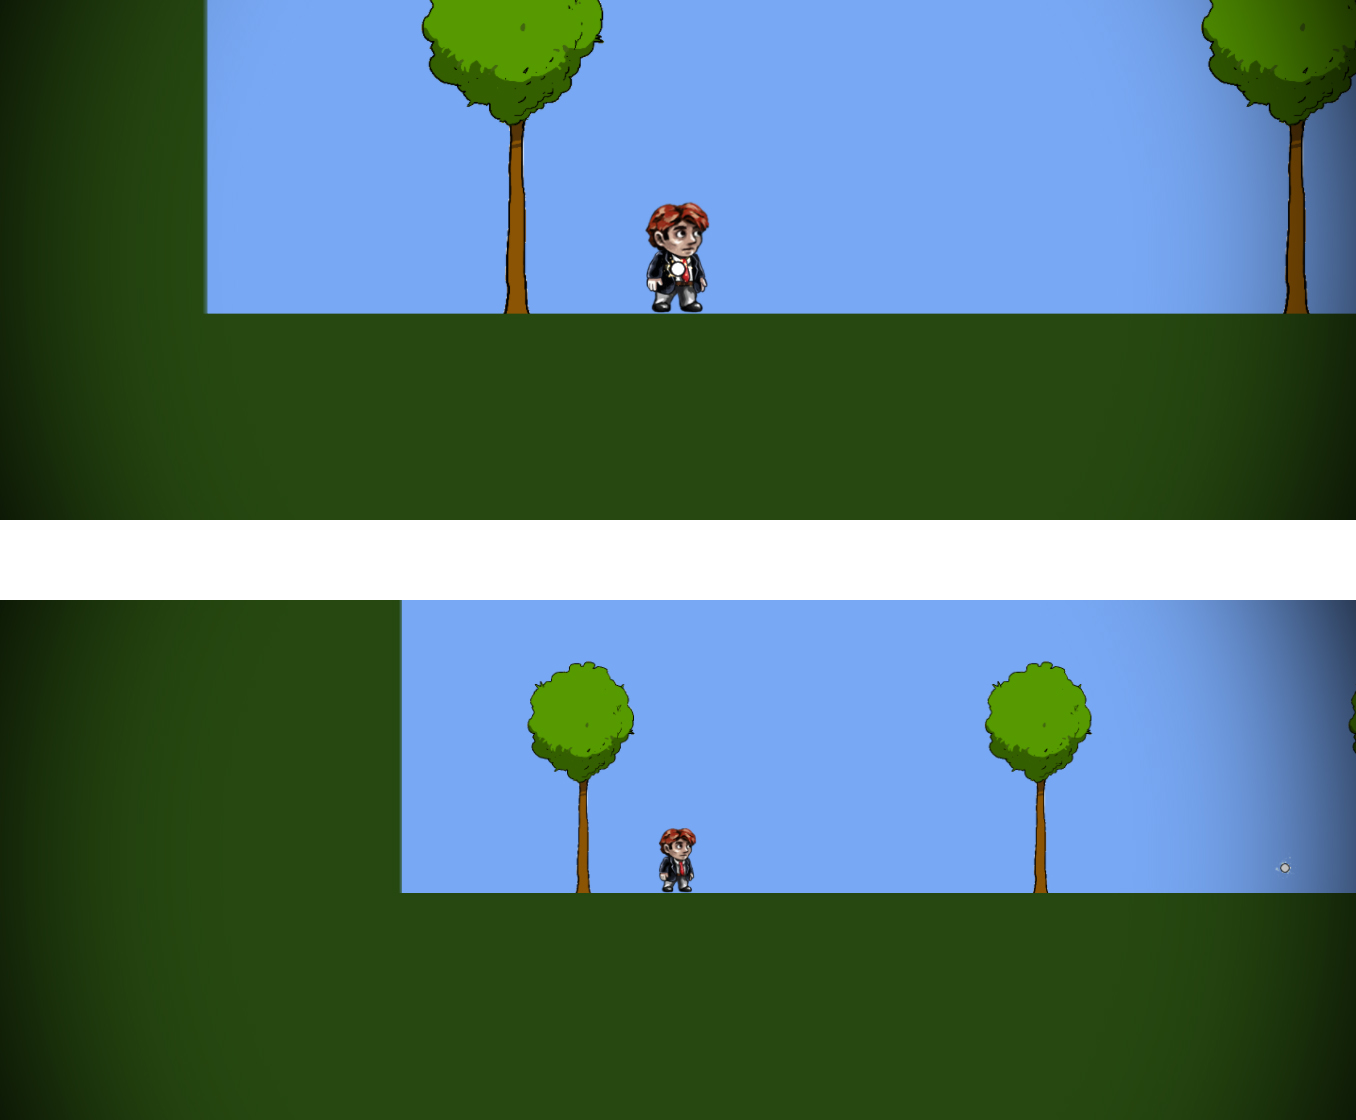
\includegraphics[width= 0.85\columnwidth]{images/gameDesign/16.jpg}
	\caption{Allontanamento della camera in relazione alla posizione del personaggio e del puntatore.}
	\label{fig:camera_allontanamento}
\end{figure}

Abbiamo ulteriormente accentuato l’effetto di disturbo provando ad applicare un approccio ibrido, limitando perciò l’allontanamento della camera, ma accompagnandolo da uno spostamento della camera lungo l’asse tra il personaggio ed il puntatore. È stata perciò scartato la possibilità di sfruttare entrambi gli approcci.

Concludendo le nostre analisi, abbiamo scelto di applicare il primo approccio proposto, spostando perciò la posizione della camera in un punto compreso tra il personaggio ed il puntatore, aumentando però il rapporto tra le due porzioni di segmento (0.37 anziché 0.25), così da poter inquadrare anche elementi più lontani. La camera raggiunge però tale posizione in un tempo particolarmente lento, così da ottenere un effetto più gradevole e spingere il giocatore a muovere il puntatore verso l’esterno dello schermo.

Il puntatore, graficamente, come è possibile vedere in Figura~\ref{fig:camera_posizione_1_4} e Figura~\ref{fig:camera_allontanamento}, è rappresentato come un semplice cerchio bianco, da cui parte un minimale effetto particellare, così da renderlo più visibile.
Abbiamo inoltre ritenuta valida la scelta di far girare il personaggio nella direzione del puntatore così che enfatizzi la metafora dell’elemento come modo per osservare altre porzioni di scena.

Mentre il personaggio è fermo, il puntatore rimane sempre visibile a schermo e la camera si adatta alla posizione di personaggio e puntatore, come analizzato nei precedenti paragrafi. In una prima versione sviluppata, il puntatore risultava essere sempre visibile, e con la camera che si muoveva di conseguenza. Successivamente abbiamo valutato la possibilità di far scomparire il puntatore in determinate situazioni, così da escluderlo dalla componente platform del gioco, che non richiede un'eccessiva osservazione di elementi non immediatamente visibili a schermo, ed associarlo invece maggiormente alla componente puzzle.
Quindi nel momento in cui il personaggio effettua un qualsiasi movimento, il puntatore scompare e la camera torna ad adattarsi, con un movimento molto lento, alla posizione del personaggio.
Il puntatore rimane visibile durante i movimenti del personaggio solamente se questo è mosso manualmente dall’utente, che vuole perciò continuare ad osservare la scena pur non rimanendo completamente fermo.
Abbiamo ritenuto che tali scelte di design, per quanto riguarda il puntatore ed il relativo movimento di camera, abbiano portato ad un buon risultato, che è stato sempre apprezzato durante le fasi di testing del prodotto.

\subsection{Meccaniche ispirate all'ambito del pre-Cinema}
\label{sec:meccaniche_precinema}

Ispirandoci all’ambito del pre-cinema e ad alcuni strumenti utilizzati nel contesto, abbiamo valutato la possibilità di includere elementi di gameplay atipici e che quindi avrebbero potuto colpire il giocatore per inventiva ed originalità.

La Lanterna Magica (riferimento) è stata scelta per costituire la meccanica innovativa più rilevante del videogioco. Considerando la sua capacità di creare immagini che al pubblico sembravano reali, abbiamo valutato la possibilità di fare in modo che il personaggio potesse plasmare il mondo a suo piacimento proiettando immagini.
La Lanterna Magica utilizza dei vetrini che vengono proiettati sulle superfici attraverso l’utilizzo di un raggio di luce. Tali vetrini spesso erano composti da più parti. Una delle prime meccaniche che abbiamo quindi valutato è stata quella di raccogliere, lungo un livello, dei frammenti di vetrino che avessero permesso, una volta ricomposti, di utilizzare la lanterna per uscire dal livello.
Tale elemento di gameplay però, avrebbe limitato l’utilizzo della Lanterna Magica esclusivamente all’ultima parte del livello, mettendone in secondo piano le potenzialità. Abbiamo perciò scartato questa ipotesi di utilizzo, nonostante in parte sia alla base dello sviluppo dell’hub centrale (riferimento).

\begin{figure}%[h]
	\centering
	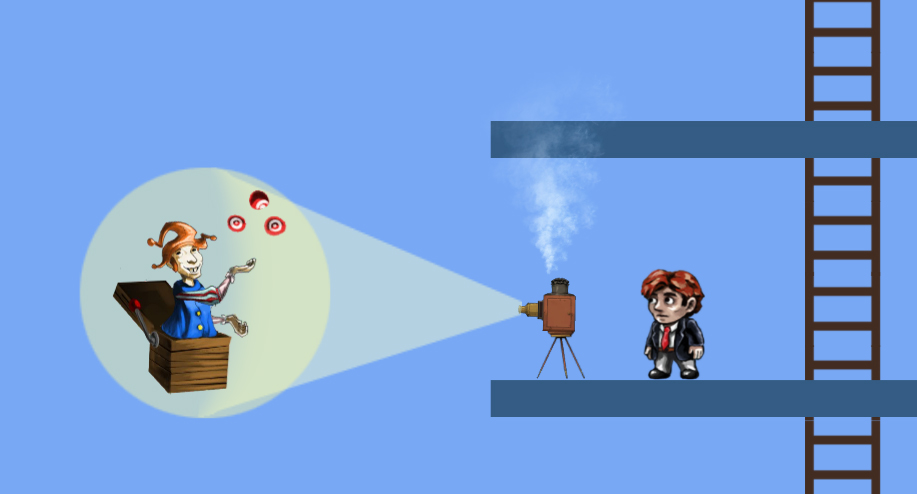
\includegraphics[width= 0.85\columnwidth]{images/gameDesign/17_giocoliere.jpg}
	\caption{Proiezione di Lanterna Magica.}
	\label{fig:meccaniche_precinema_lanterna01}
\end{figure}

Si è perciò valutata la possibilità di poter utilizzare in ogni momento la Lanterna Magica, magari dovendo raccogliere il vetrino da poter utilizzare lungo il livello. Si sono fatte alcune ipotesi per valutare le potenzialità di questo approccio, ed i risultati, ottenuti anche da alcuni test, sono subito sembrati molto promettenti.
Una delle iniziali idee proposte, è stata quella di usare due particolari proiezioni in grado di poter attirare (Figura~\ref{fig:meccaniche_precinema_lanterna01}) o spaventare i nemici, così da spingerli a svolgere determinate azioni o magari distogliere il loro sguardo dal personaggio.



È evidente come la lanterna magica sia uno strumento che, potendo proiettare nello scenario un qualsiasi tipo di elemento, apre le porte ad un amplissimo numero di possibilità di gioco.
Il passaggio successivo è stato quindi quello di cercare delle proiezioni che avessero permesso di avere meccaniche semplici da utilizzare, ma con un buon potenziale per lo sviluppo di sezioni ed enigmi di gioco. Tra quelle che abbiamo valutato ci sono, a titolo di esempio:

\begin{itemize}
	\item \textbf{Piattaforma.} Permette al personaggio di saltarci sopra per raggiungere posti non raggiungibili. È la forma più basilare di modifica all’ambiente. Aggiunge un elemento già esistente nello scenario, non richiede quindi uno sforzo di comprensione eccessivo. Può essere utilizzata anche come passerelle per un nemico.
	
	\item \textbf{Molla.} Una sorta di piattaforma potenziata. Permette di ricevere una spinta verso l’alto proporzionale all’altezza di caduta e perciò di raggiungere posti ancora più elevati. Apre alcune possibilità di gameplay ulteriori rispetto alla piattaforma, in quanto esiste anche la possibilità di raggiungere posti differenti a seconda dell’altezza da cui inizia la caduta sulla molla.
	
	\item \textbf{Fantasma.} Spaventa i nemici. Permette di distrarre i nemici dal personaggio, oltre che spingerli verso un possibile obiettivo (bottone da premere). Si è inoltre, coerentemente con questa proiezione, valutata la possibilità di inserire tipologie di nemici che avessero reagito in maniera differente alla visione del fantasma, come nemici corazzati che per lo spavento avessero perso l’armatura e quindi diventati vulnerabili.
	
	\item \textbf{Esca (giocoliere).} Il giocoliere era una proiezione utilizzata anche nei tipici spettacoli di lanterna magica dell’epoca, quindi aggiunge anche un elemento di coerenza storica. Può essere utilizzato con le stesse modalità del fantasma, cioè per spingere il nemico verso un possibile obiettivo dello scenario.
	
	\item \textbf{Acquario.} Inizialmente è stato pensato come elemento che può essere utilizzato per rallentare tutto ciò che ne passa attraverso. Una cassa in caduta può quindi essere rallentata per permettere al personaggio di svolgere altre azioni. Successivamente si è valutata la possibilità di usarlo come elemento capace di generare confusione in un nemico, attraverso correnti imprevedibili al suo interno.
	
	\item \textbf{Vento.} Genera un potente flusso di vento che interagisce con l’ambiente di gioco. Può essere usato per spingere il personaggio, per rallentare i nemici, per spostare elementi dello scenario o per interagire con meccanismi sviluppati appositamente (girandole che aprono porte, mongolfiere).
	
	\item \textbf{Gabbia per nemici.} Capace di intrappolare un nemico per un breve periodo di tempo.
	
	\item \textbf{Guardaroba.} Traveste il nemico da personaggio principale e viceversa, così da confondere il comportamento degli altri nemici.
	
	\item \textbf{Burrone con spuntoni.} Permette di uccidere i nemici.
	
	\item \textbf{Fiamma.} Permette di uccidere i nemici e di interagire con elementi appositi (palloncini).
	
	\item \textbf{Picchio di legno.} Permette di interagire a distanza con leve ed altri meccanismi.
\end{itemize}

Le precedenti proiezioni sono state valutate attentamente, cercando di prendere in considerazione tutte le possibilità di gameplay che avrebbero potuto originare.
Considerando anche la struttura generale di gioco ed il numero di livelli che abbiamo stimato fossero necessari per fornire un’esperienza sufficiente (riferimento), abbiamo deciso di utilizzare le proiezioni della piattaforma e del vento (Figura~\ref{fig:meccaniche_precinema_piattaforma_vento}), in quanto la prima risulta di facile comprensione ed utilizzo, mentre la seconda mostra le vere potenzialità della lanterna magica e gli effetti che questa può creare nello scenario di gioco.

\begin{figure}%[h]
	\centering
	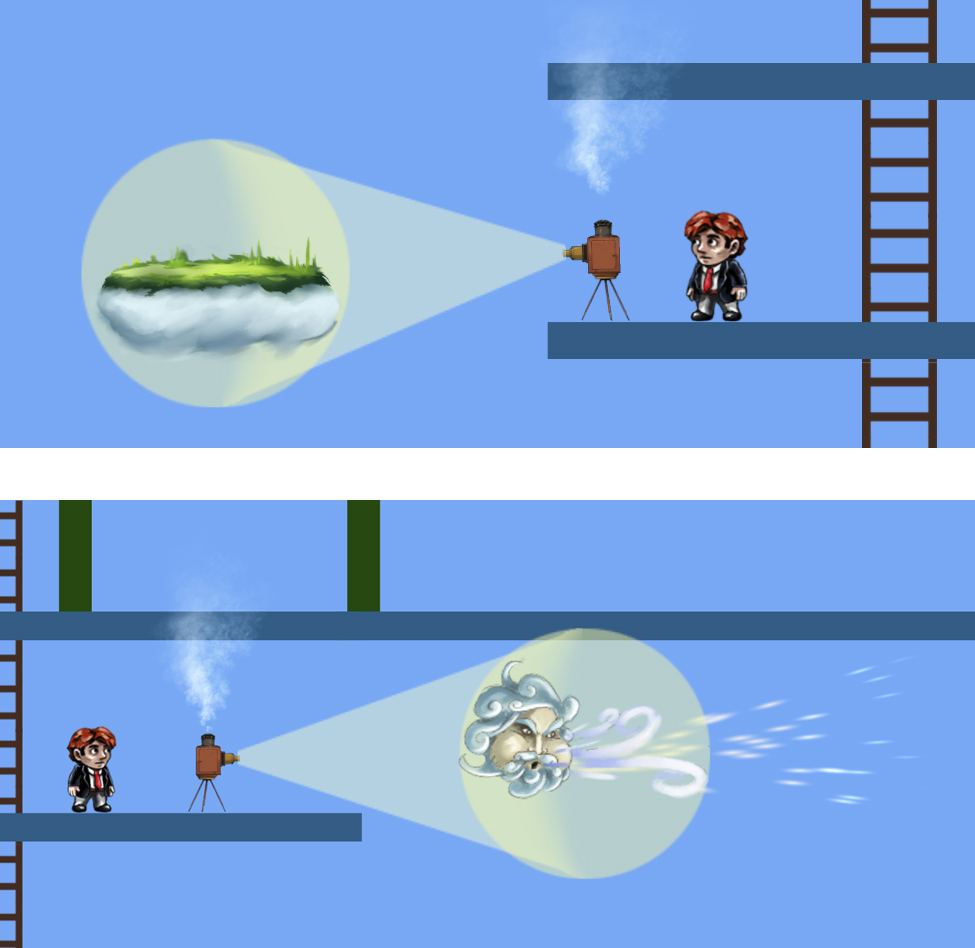
\includegraphics[width= 0.85\columnwidth]{images/gameDesign/18_piattaforma_vento.jpg}
	\caption{Proiezioni di vento e piattaforma.}
	\label{fig:meccaniche_precinema_piattaforma_vento}
\end{figure}

Per quanto riguarda la piattaforma, questa può essere attraversata dal basso verso l’alto, grazie ad un salto del personaggio, questo per evitare che il suo utilizzo non sia troppo complicato e l’operazione non risulti troppo frustrante. Come si può vedere in Figura~\ref{fig:meccaniche_precinema_piattaforma_vento}, abbiamo quindi deciso di renderla graficamente come una nuvola con, appoggiata su di essa, una porzione di terreno. Il giocatore ha quindi la sensazione di un terreno soffice, attraversabile, nella parte più bassa, mentre duro e concreto nella parte superiore.
Come già specificato, abbiamo utilizzato la piattaforma in quanto si tratta di un elemento di facile utilizzo e comprensione. Le piattaforme sono già presenti nello scenario di gioco, l’utente non si trova quindi spiazzato dalla sua presenza. Si trova però a dover ragionare sulla giusta posizione in cui porre la proiezione per far sì che questa sia di una qualche utilità.
Come verrà spiegato nell’analisi dei livelli (riferimento) si è preferito mostrare all’utente la lanterna e la relativa proiezione della piattaforma prima di dargli la possibilità di raccoglierla e quindi usarla. Questo per permettere un iniziale ambientamento del giocatore con la particolare meccanica di gioco e mostrare alcuni possibili utilizzi che potrebbero risultare poco intuitivi se richiesti direttamente all’utente.

La piattaforma viene utilizzata sia dal personaggio giocabile per raggiungere posti troppo lontani o per spostare nemici da una parte all’altra della scena, così da poter premere bottoni o interagire con l’ambiente nel modo previsto, come mostrato in Figura~\ref{fig:meccaniche_precinema_piattaforma}.

\begin{figure}%[h]
	\centering
	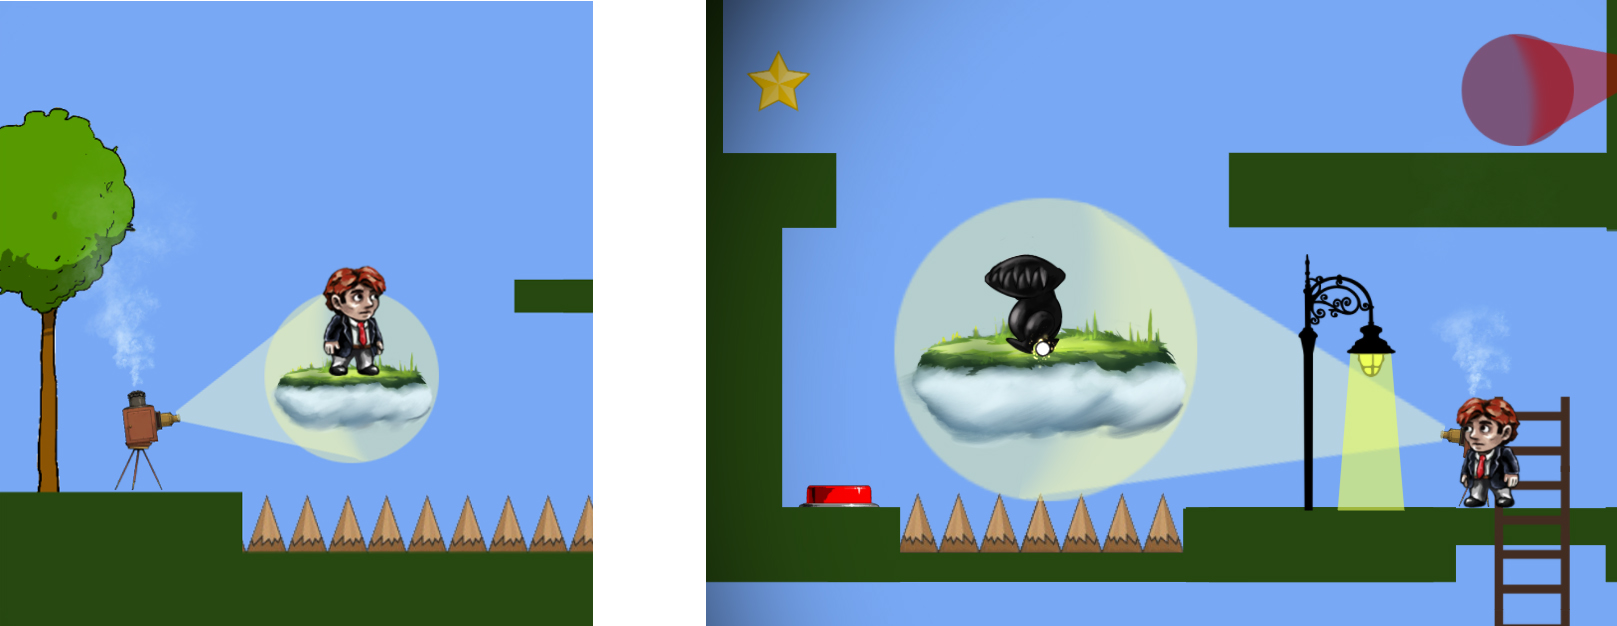
\includegraphics[width= \columnwidth]{images/gameDesign/19_piatt.jpg}
	\caption{Utilizzi della proiezione della piattaforma.}
	\label{fig:meccaniche_precinema_piattaforma}
\end{figure}

La proiezione del vento è invece caratterizzata dal fatto di interagire anche con l’ambiente e quindi non esclusivamente col personaggio di gioco. Gli alberi reagiscono al suo utilizzo, così come le foglie, le bandiere e le girandole presenti nel livello.
Come per la piattaforma, prima di permettere all’utente di usare la meccanica del vento, glie ne viene mostrato l’utilizzo in più forme.
Il vento può dare una spinta ulteriore al personaggio, permettendogli quindi di spiccare salti che possono coprire grandi distanze. Può quindi raggiungere zone molto elevate o saltare grandi burroni.
Tale proiezione può essere anche utilizzata per rallentare o velocizzare i nemici, a seconda del suo verso, per interagire con alcuni elementi dell’ambiente, sia in maniera puramente estetica, come i già citati alberi e bandiere, o per attivare meccanismi utili alla partita, come girandole che permettono l’apertura di speciali porte, mongolfiere con le quali è possibile raggiungere la cima di una montagna o barche a vela che permettono di superare distese d’acqua (Figura~\ref{fig:meccaniche_precinema_vento}).

Il vento è sicuramente una meccanica molto interessante, che esprime massimamente l’idea di sorpresa generabile da una proiezione di lanterna magica.

\begin{figure}%[h]
	\centering
	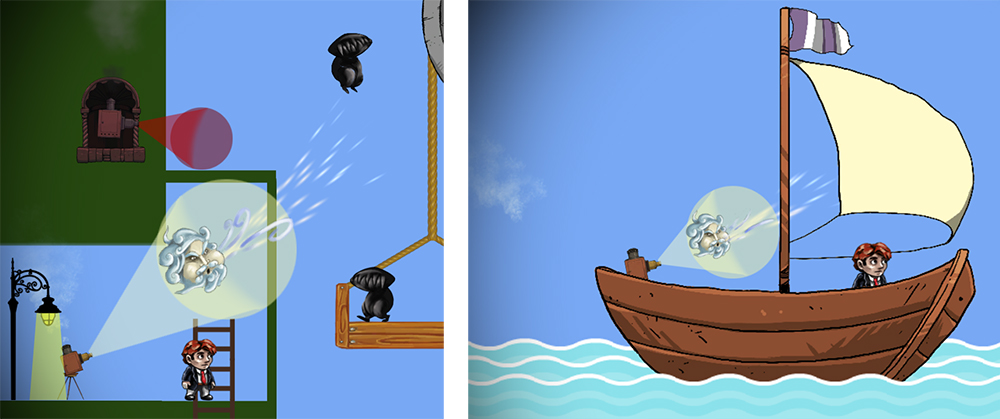
\includegraphics[width= \columnwidth]{images/gameDesign/20_vento.jpg}
	\caption{Utilizzi della proiezione del vento.}
	\label{fig:meccaniche_precinema_vento}
\end{figure}

Esempi di utilizzo delle due meccaniche verranno mostrati nell’analisi dei livelli (riferimento).

Inizialmente si ipotizzava di far utilizzare la lanterna assegnandole uno specifico tasto da tenere premuto. La lanterna sarebbe stata quindi sempre in mano al personaggio ed utilizzata in qualsiasi momento. Tale approccio si sposa perfettamente con alcune proiezioni, come quelle di fantasma ed esca, in quanto l’utente può muovere dinamicamente l’elemento proiettato e direzionarlo in relazione ai movimenti dei nemici, ma impedisce di utilizzare molte delle altre proiezioni teorizzate, in quanto non permette una diretta interazione di queste con il personaggio giocabile.

La soluzione che abbiamo ritenuto più valida è stata quindi quella di permettere al giocatore di poter mirare attraverso la pressione di un tasto, e proiettare al suo rilascio. In questo stesso momento la lanterna magica viene lasciata a terra e continua a proiettare, fino a che il giocatore non decida di riprenderla di nuovo in mano.
Il momento dedicato alla mira, sfrutta l’utilizzo di una sagoma dell’elemento che si andrà a proiettare, così da dare immediatamente al giocatore la sensazione di come e dove verrà creato l’oggetto dello scenario.
Il concetto di mira è stato sviluppato parallelamente all’attuale implementazione di camera e puntatore, in quanto la sagoma dell’oggetto da proiettare compare esattamente nella stessa posizione del puntatore, così da non confondere l’utente con metafore di gioco differenti.
Come si può vedere in Figura~\ref{fig:meccaniche_precinema_swapper}, per tale meccanica ci si è ispirati al videogioco The Swapper (riferimento).

\begin{figure}%[h]
	\centering
	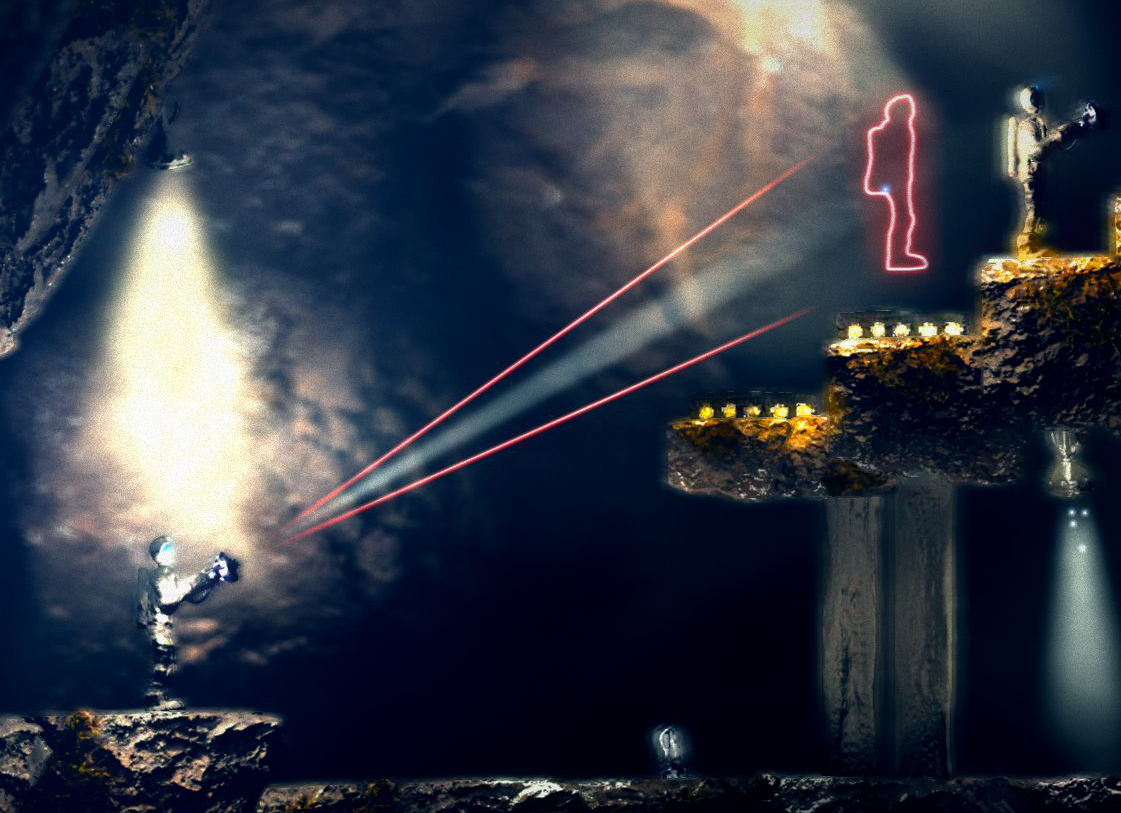
\includegraphics[width= 0.85\columnwidth]{images/gameDesign/21_swapper.jpg}
	\caption{Concetto di mira espresso in The Swapper.}
	\label{fig:meccaniche_precinema_swapper}
\end{figure} 

Un altro elemento di gioco ispirato alla Lanterna Magica è quello che abbiamo definito come \textit{mondo in divenire}.
Come già specificato, la lanterna utilizzava dei vetrini, che potevano anche essere inseriti e rimossi durante gli spettacoli, così da permettere un evolversi delle ambientazioni e di un’eventuale storia da raccontare. Queste operazioni facevano in modo che alcuni elementi apparissero o scomparissero con un effetto di dissolvenza.

Sviluppando perciò il mondo di gioco come se questo fosse un vero spettacolo di lanterna magica, abbiamo ritenuto di poter ottenere un effetto grafico suggestivo e curioso, includendo la possibilità di poter far evolvere lo scenario di gioco con l’apparizione e la scomparsa di elementi in dissolvenza.
Questo processo è stato, in un primo momento, relazionato al raccoglimento di stelle. Il giocatore poteva quindi porsi come obiettivo quello di raggiungere una stella, così da poter far evolvere il mondo di gioco e poter proseguire con il livello.

Dopo un attenta valutazione ed alcuni test effettuati, abbiamo deciso di abbandonare questa strada, anche in relazione all’inserimento di altre tipologie di collezionabili, il cui numero, sommato a quello delle stelle, avrebbe potuto confondere il giocatore per quanto concerne il ruolo di ogni elemento da raccogliere. Inoltre, era presente il rischio che il giocatore avesse dato priorità ad un obiettivo locale, il raccoglimento della stella, e perdere di vista obiettivi più generici di gioco.
Nella attuale implementazione, quindi, l’evoluzione del mondo di gioco è assegnata a dei semplici \textit{trigger} attivati dal passaggio del personaggio (Figura~\ref{fig:meccaniche_precinema_dissolving}). Il posizionamento di tali elementi è chiaramente stato fatto con attenzione e dopo attente fasi di analisi e studio dei livelli.

\begin{figure}%[h]
	\centering
	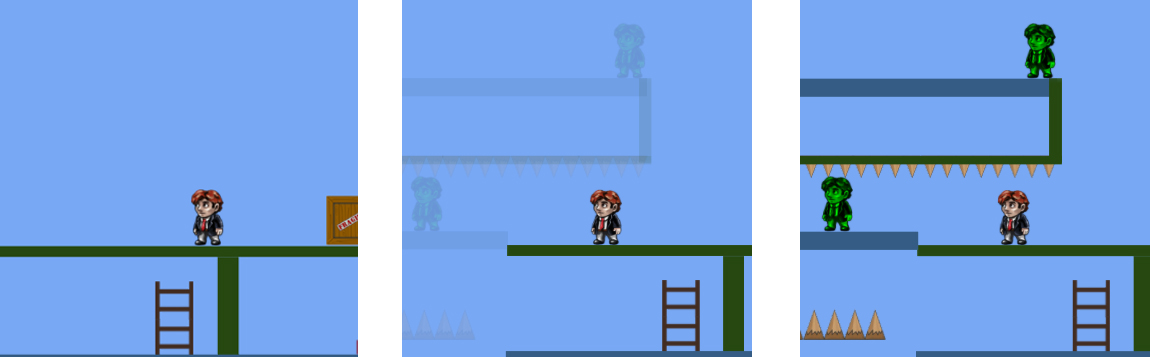
\includegraphics[width= \columnwidth]{images/gameDesign/22.jpg}
	\caption{Meccanica delle Dissolving Views.}
	\label{fig:meccaniche_precinema_dissolving}
\end{figure} 

Le meccaniche di gioco primarie, come abbiamo analizzato, sono quindi quelle \textit{platform} e \textit{puzzle}, enfatizzate dall’utilizzo della Lanterna Magica che permette di interagire ed alterare lo scenario.
Tali elementi di gameplay sono stati però affiancati da altre meccaniche ispirate al contesto del \textit{pre-cinema}.
Tra gli elementi \textit{serious} del nostro videogioco, abbiamo incluso la possibilità di raccogliere degli oggetti e quindi lo sbloccare le relative schede informative che ne descrivono la storia, l’utilizzo ed eventuali curiosità a riguardo (riferimento).

Nei test effettuati (riferimento) abbiamo però notato come i ragazzi fossero poco attratti dall’apertura delle schede informative e quindi dall’apprendere determinati concetti che riteniamo importanti per l’esperienza di gioco e per l’obiettivo di Tesi prefissato.
Abbiamo quindi deciso di inserire diversi elementi aggiuntivi, tra questi alcune meccaniche di gioco, studiate appositamente, per rendere più interessante il raccoglimento di tali oggetti e quindi stimolare curiosità per l’apertura delle relative schede informative.

La camera oscura (riferimento) è un particolare strumento che riproduce all’interno di una delle sue facce, l’immagine capovolta di quanto si trova di fronte al foro della faccia opposta.
Al raccoglimento dell’oggetto relativo perciò, il personaggio si trova in una porzione di gioco già affrontata, per assicurarci che abbia dei riferimenti che non lo facciano trovare spaesato, ma con la camera ruotata di 180 gradi (Figura~\ref{fig:meccaniche_precinema_camera_oscura}). Il giocatore si trova quindi a dover far muovere il personaggio ma facendo attenzione al fatto che i comandi sono invertiti rispetto alla partita svolta fino a quel momento.

\begin{figure}%[h]
	\centering
	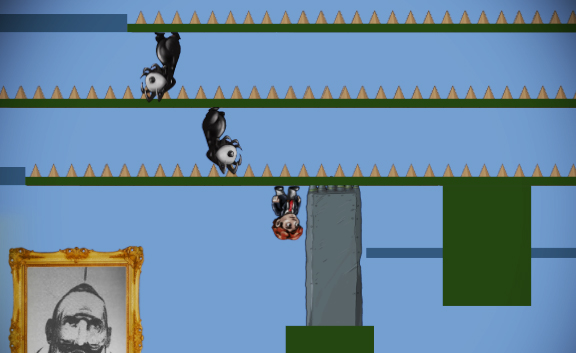
\includegraphics[width= 0.8\columnwidth]{images/gameDesign/23_cameraOscura.jpg}
	\caption{Meccanica della Camera Oscura.}
	\label{fig:meccaniche_precinema_camera_oscura}
\end{figure} 

Al termine di questa breve sezione, viene sbloccata la scheda informativa relativa alla camera oscura, così che l’utente possa informarsi maggiormente nel caso sia abbastanza stimolato a farlo.

Per quanto riguarda le lenti, abbiamo inserito degli approfondimenti che parlano di quelle convergenti e divergenti.
Per far sì che l’oggetto venga contestualizzato all’interno del mondo di gioco, abbiamo studiato un’apposita sezione in cui il personaggio venga rimpicciolito ed ingrandito dal passaggio attraverso delle lenti (Figura~\ref{fig:meccaniche_precinema_lenti}) e si trovi quindi a relazionarsi con elementi di gioco di diverse dimensioni, come delle fessure sui muri, che possono essere affrontati solo se si è passati attraverso la giusta sequenza di lenti.

\begin{figure}%[h]
	\centering
	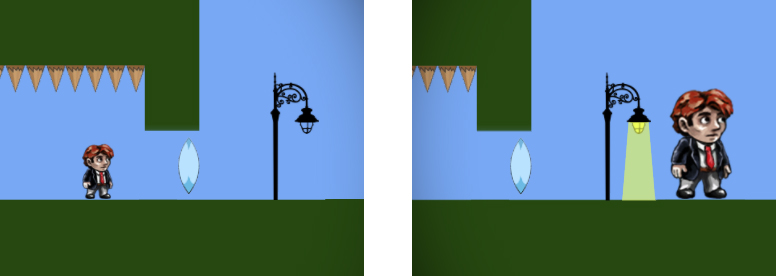
\includegraphics[width= 0.9\columnwidth]{images/gameDesign/24_lenti.jpg}
	\caption{Meccanica delle Lenti.}
	\label{fig:meccaniche_precinema_lenti}
\end{figure} 

Stiamo inoltre valutando la possibilità di includere le suddette meccaniche anche in altre sezioni di gioco. Bisogna sicuramente stare attenti a sfruttarle in maniera intelligente, senza rischiare di esser confusionari e confondere l’utente. Sono state introdotte per stimolare il giocatore ad aprire le schede informative al momento del raccoglimento del relativo oggetto, se dovessero essere inserite in altre sezioni di gioco, dovremmo evitare di avvicinarle ad altri elementi contestualizzanti per non mescolare concetti tra di loro, oltre che usarle con parsimonia per non caricare il giocatore di troppe meccaniche da dover padroneggiare.

\subsection{Elementi di rigiocabilità}
\label{sec:elementi_rigiocabilita}

Con elementi di rigiocabilità vogliamo intendere tutti quei componenti che possono spingere il giocatore a ricominciare livelli di gioco (o il gioco stesso) una volta che questi siano già stati portati a termine.
Nel nostro caso, gli elementi di rigiocabilità più diretti che abbiamo voluto inserire sono le stelle ed i collezionabili. La Figura~\ref{fig:rigiocabilita_stelle_collezionabili} ne mostra degli esempi.

All’interno dei livelli sono presenti degli oggetti che, una volta raccolti, sbloccano la relativa scheda informativa, sono quindi elementi coerenti col contesto, li chiameremo in maniera generica “collezionabili”. Questi sono facilmente raggiungibili dal personaggio principale. Sono generalmente ben visibili e spesso si trovano lungo il percorso primario. Essendo elementi importanti per la componente \textit{serious} del gioco, si vuole evitare che il giocatore li salti per distrazione, ma anzi sia stimolato a raccoglierli e ad informarsi riguardo ciò che ha appena raccolto.

Le stelle sono invece elementi raggiungibili in maniera più difficile, richiedono sempre delle abilità di reazione, di movimento o di ragionamento superiori rispetto ai semplici collezionabili. Il loro unico scopo è quello di permettere l’assoluto completamento del livello.

\begin{figure}%[h]
	\centering
	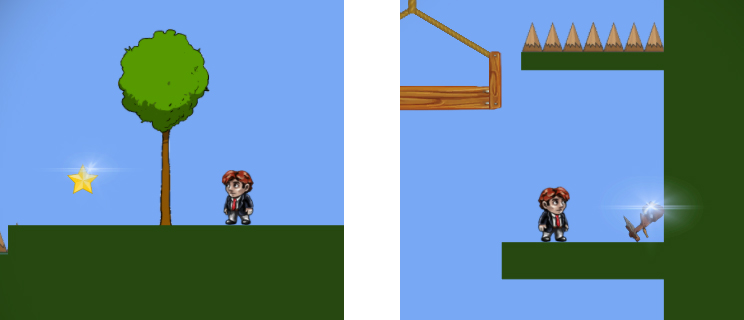
\includegraphics[width= 0.9\columnwidth]{images/gameDesign/25_stelle_collezionabili.jpg}
	\caption{Stelle ed oggetti collezionabili.}
	\label{fig:rigiocabilita_stelle_collezionabili}
\end{figure} 

È importante chiarire che sia i collezionabili che le stelle non risultano essenziali alla conclusione di un livello. Il giocatore può arrivare anche al termine senza averne raccolti. L’interazione del personaggio con questi elementi non influisce sul naturale svolgimento della partita e non genera nessuna conseguenza sullo scenario di gioco, esclusi i casi di collezionabili contestualizzati, che abbiamo precedentemente analizzato (\ref{sec:meccaniche_precinema}). Stiamo comunque valutando la possibilità di inserire alcuni di questi elementi in maniera obbligatoria, o per insegnare al giocatore determinate meccaniche di gioco, o per spingerlo a leggere alcune schede informative.

Le stelle sono elementi presenti in moltissimi altri giochi, primo fra tutti SuperMario. Il giocatore è naturalmente spinto a raccoglierle, senza bisogno di ulteriori spiegazioni.

Valiant Hearts (riferimento) è il videogioco a cui ci siamo maggiormente ispirati per la componente \textit{Serious}, quindi, anche per la struttura dei collezionabili, così come sono stati descritti, abbiamo cercato di rifarci al gioco. Anche in Valiant Hearts il raccoglimento di determinati oggetti porta allo sbloccare schede informative che possono essere consultate liberamente dall’utente.
Come mostrato in Figura~\ref{fig:rigiocabilita_UI_hub}, il numero di collezionabili e stelle raccolte, viene mostrato nell’hub centrale (riferimento) al passaggio del personaggio di fronte alle varie porte che conducono ai livelli. Il giocatore quindi, vedendo che un livello già giocato non risulta interamente completato, è naturalmente spinto a rigiocarlo, cercando di scoprirne tutti i segreti e quindi portarlo a termine.

\begin{figure}%[h]
	\centering
	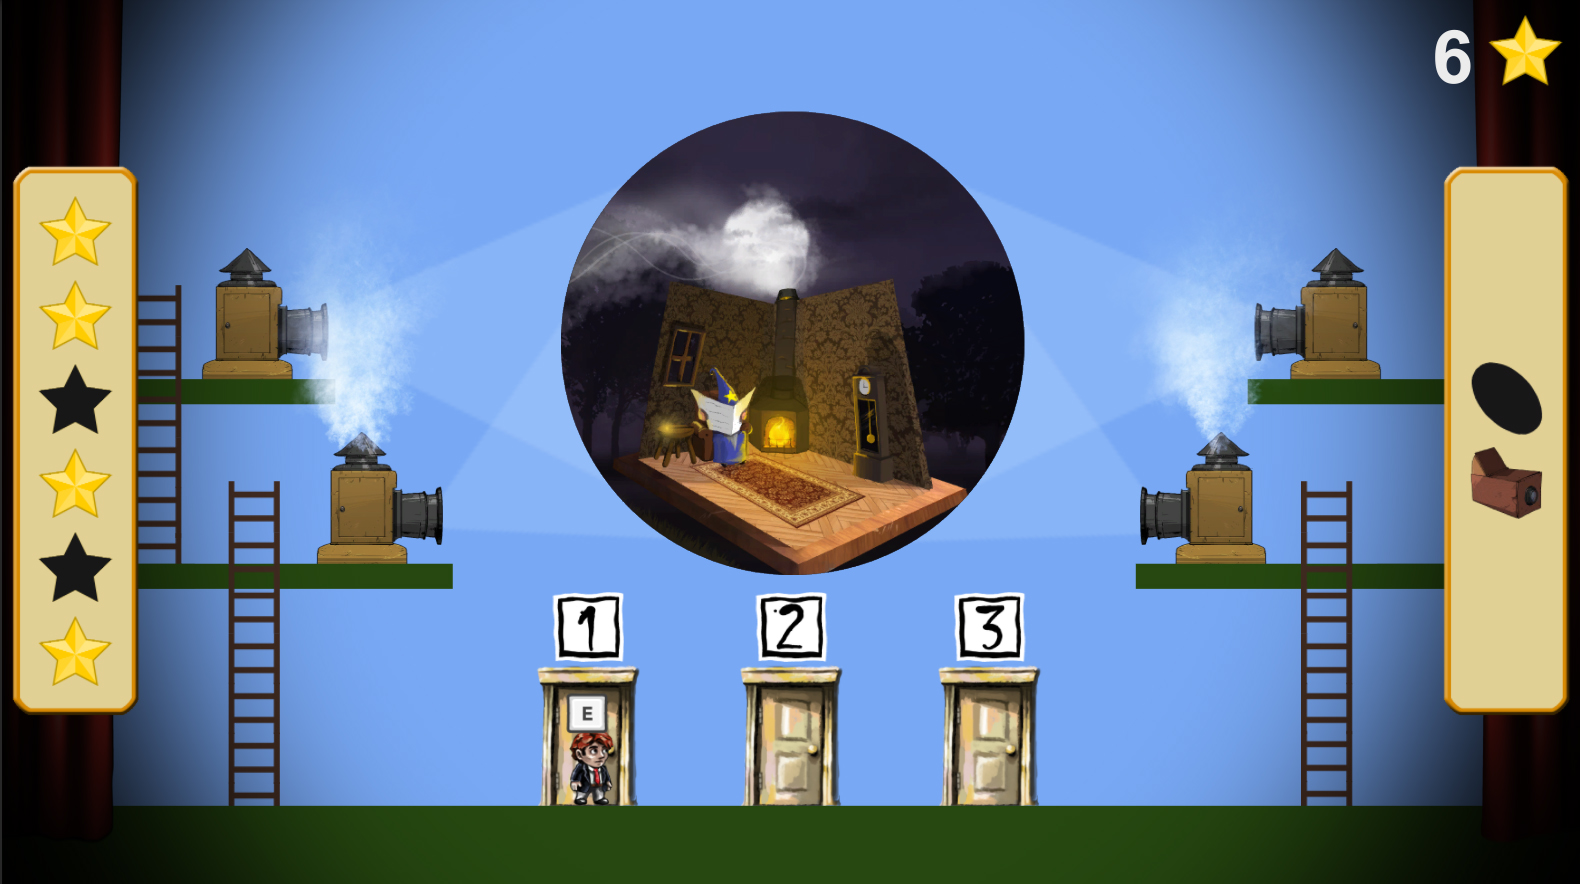
\includegraphics[width= 0.9\columnwidth]{images/gameDesign/26_hub.jpg}
	\caption{UI che indica i collezionabili e le stelle raccolte in ogni livello.}
	\label{fig:rigiocabilita_UI_hub}
\end{figure} 

Altri elementi di rigiocabilità sono banalmente il divertimento provato dal giocatore e le varie possibilità di interazione che ha con lo scenario.
Se una partita risulta particolarmente divertente, l’utente può essere portato a ricominciare, anche se l’esperienza di gioco può risultare non troppo differente dall’ultima partita.

Inoltre, la presenza di elementi non utili alla conclusione di un livello, ma capaci di generare curiosità e stupore nel giocatore, possono spingerlo a riprovare l’esperienza di gioco, che può risultare arricchita ad ogni successiva partita.
Ad esempio, nel terzo livello di gioco (riferimento), sono presenti, nelle prime sezioni, degli alberi che reagiscono al vento, piegandosi e lasciando foglie che fluttuano in aria. Successivamente si entra in una sezione al chiuso, in cui si raccoglie la lanterna magica ed il relativo vetrino che proietta l’immagine di Eolo che genera vento dalla sua bocca. Proseguendo con il livello, si potrà di nuovo uscire all’esterno, questa volta senza la presenza di vento, saranno comunque visibili dei nuovi alberi. Il giocatore può tranquillamente proseguire con la partita senza notarli. Ma, ad un successivo gameplay, può provare ad utilizzare la proiezione del vento e vedrebbe che tali alberi reagiscono, piegandosi e generando foglie, che sono addirittura influenzate dalla proiezione (Figura~\ref{fig:rigiocabilita_foglie}). Il giocatore può quindi perdere del tempo provando a giocare con le foglie e facendole volare a proprio piacimento.

\begin{figure}%[h]
	\centering
	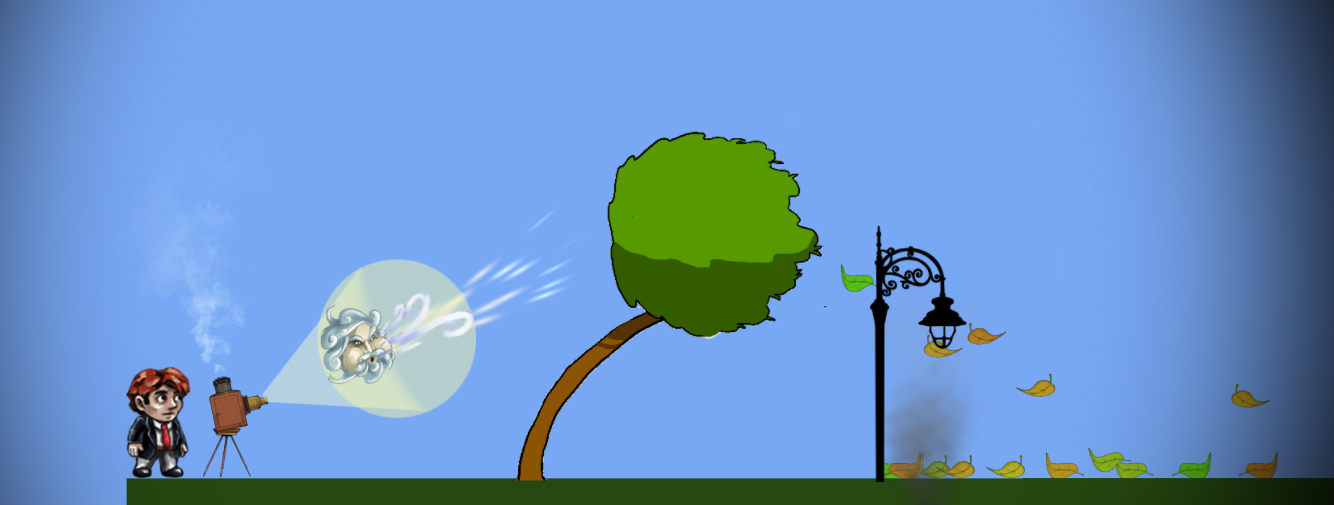
\includegraphics[width= 0.9\columnwidth]{images/gameDesign/27_foglie.jpg}
	\caption{Foglie mosse dalla proiezione del vento.}
	\label{fig:rigiocabilita_foglie}
\end{figure} 

\section{Ambiente e personaggi}
\label{sec:ambiente_personaggi}

Il design di ambientazione e personaggi è stato in parte svolto prima dell’inizio del lavoro di Tesi. In tale periodo, il design realizzato da esperti nel settore del \textit{Gaming} è stato accompagnato dal supporto di un reparto grafico che ha permesso anche un dialogo prolifico per quanto riguarda il \textit{character design} e lo sviluppo di caratteristiche ambientazioni. Tale supporto è stato presente in forma minore durante il lavoro di Tesi, in quanto il reparto grafico si è soprattutto occupato di fornire \textit{asset} utili allo sviluppo pratico del videogioco. Il Design, da questo punto di vista, si è perciò limitato a sottolineare alcuni elementi emersi durante le precedenti sessioni e a far emergere nuovi dettagli che, durante le fasi di sviluppo ed ideazione dei livelli, si sono delineati come importanti per l’immersione ed il coinvolgimento del giocatore.

Nei successivi paragrafi verranno affrontati, in maniera più approfondita, i percorsi di design dell’ambientazione e del \textit{character design} del personaggio principale e dei nemici.

\subsection{Ambientazione}
\label{sec:ambientazione}

Per quanto riguarda il design dell’ambientazione e del mondo di gioco, abbiamo deciso di ispirarci agli elementi presenti negli spettacoli dell’epoca. Il reparto grafico ha quindi realizzato delle possibili ambientazioni utili a trarre ispirazione anche per le fasi di design delle meccaniche e dei personaggi.

L’idea preliminare di gioco era quella di avere un personaggio con l’abilità di trovarsi ed attraversare vari mondi, ognuno caratterizzato da un proprio tema. Ognuna di queste ambientazioni sarebbe quindi stata descritta da uno stile grafico pertinente allo spettacolo da cui si era preso spunto. Coerentemente con l’ambiente, anche lo stile dei personaggi e degli oggetti interagibili, sarebbe cambiato per assicurare una coinvolgente armonia visiva. Ogni ambiente di gioco sarebbe quindi stato caratterizzato da meccaniche differenti, in armonia con l’aspetto grafico.
In Figura~\ref{fig:ambientazione_teatro_ombre} viene mostrata un'ambientazione ispirata agli spettacoli del teatro delle ombre. Queste sezioni sarebbero state caratterizzate da un gameplay basato fortemente sul contrasto tra zone di luce e di ombra, da utilizzare per evitare di essere visti da i nemici. Chiaramente tale meccanica sarebbe potuta essere sfruttata anche dai nemici, che, come si può vedere dall’immagine sono caratterizzati da un occhio molto luminoso. Questo, ad intervalli regolari, veniva chiuso dal nemico, che quindi si mimetizzava perfettamente nelle zone scure.

\begin{figure}%[h]
	\centering
	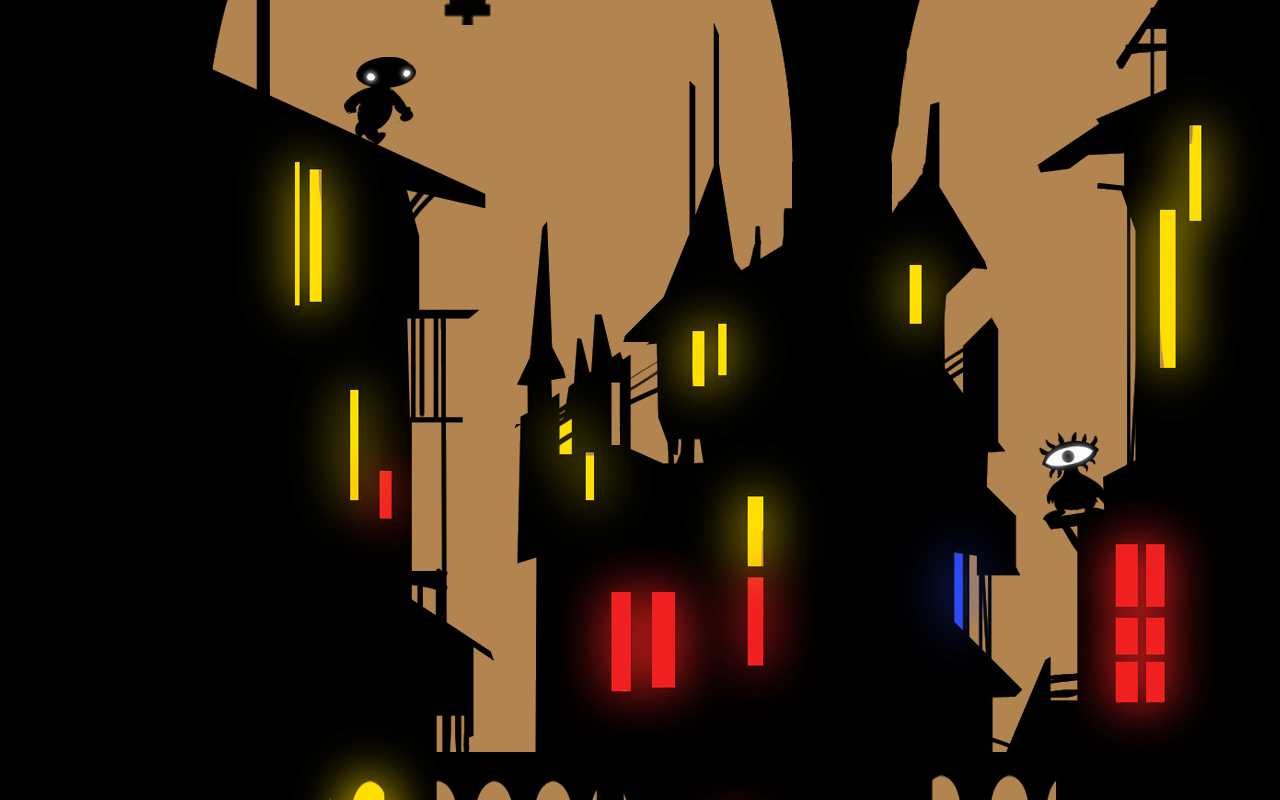
\includegraphics[width= 0.9\columnwidth]{images/gameDesign/28_cinefuochi.jpg}
	\caption{Ambientazione ispirata agli spettacoli del Teatro delle Ombre.}
	\label{fig:ambientazione_teatro_ombre}
\end{figure} 

Tale approccio però, avrebbe rischiato di frustrare il giocatore in quanto, un grande numero di meccaniche differenti, accompagnate da cambi frequenti di ambientazione, potrebbe non essere facilmente assimilabile e padroneggiabile dall’utente. Abbiamo perciò deciso di focalizzarci su una singola tematica e cercato di approfondirla così da renderla più piacevole da scoprire e con maggiori possibilità di \textit{gameplay}.
Tale ambientazione principale potrà essere accompagnata, se ritenuto necessario, anche da altre ambientazioni e relative meccaniche, che però compariranno in maniera minore, e fungeranno da accompagnamento alla vera esperienza.

L’idea sviluppata, quindi, dopo le fasi di design, è stata quella di caratterizzare l’ambiente con elementi tipici degli spettacoli di Lanterna Magica (Figura~\ref{fig:ambientazione_lanterna}). Il mondo di gioco sarà quindi visivamente abbastanza attraente, caratterizzato da colorazioni forti, con tinte pastello ed abbastanza ricche di elementi su schermo. Risulta importante ricordare che i vetrini utilizzati in questi spettacoli erano prodotti da artisti differenti, presentano perciò vari stili e metodologie di disegno. Questo permette al reparto artistico una certa flessibilità nella creazione di \textit{asset} per il videogioco, pur prendendo ispirazione da oggettistica ed elementi realmente utilizzati.

\begin{figure}%[h]
	\centering
	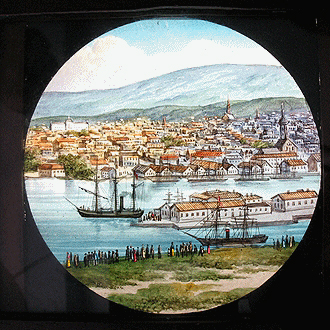
\includegraphics[width= 0.5\columnwidth]{images/gameDesign/29_lanterna.jpg}
	\caption{Vetrino di Lanterna Magica che mostra una tipica ambientazione.}
	\label{fig:ambientazione_lanterna}
\end{figure} 

Poiché lo scopo del lavoro è stato lo sviluppo di un prototipo, spesso vengono a mancare degli elementi estetici che caratterizzano invece la realizzazione di un prodotto completo. Gli sfondi che fungono da ambientazione per il mondo di gioco non sono quindi stati realizzati dal reparto grafico, in quanto non essenziali per lo sviluppo di un prototipo.
L’aspetto attuale del prodotto non ha quindi assolutamente attinenza con ciò che dovrà essere al termine dello sviluppo.
Per la verifica e l’evoluzione delle meccaniche di gioco, abbiamo quindi utilizzato sfondi ed elementi senza apporto artistico.

Graficamente, abbiamo deciso di rappresentare il terreno con colorazioni uniformi, artisticamente non rilevanti, ma comprensibili dal punto di vista del giocatore.
Abbiamo comunque ritenuto necessario un supporto grafico di buon livello per quanto riguarda gli elementi che avrebbero potuto influenzare l’esperienza di gioco degli utenti. Ci si è perciò assicurati che la comprensibilità degli elementi di gioco, tra cui l’interfaccia grafica e le componenti caratterizzanti le meccaniche di gioco, fosse sempre garantita.
Per quanto riguarda questi elementi, verranno trattati, dove necessario, nel capitolo relativo all’analisi dei livelli sviluppati.

Il prodotto finito sarà quindi dotato di ambientazioni artisticamente più valide.

%\begin{figure}%[h]
%	\centering
%	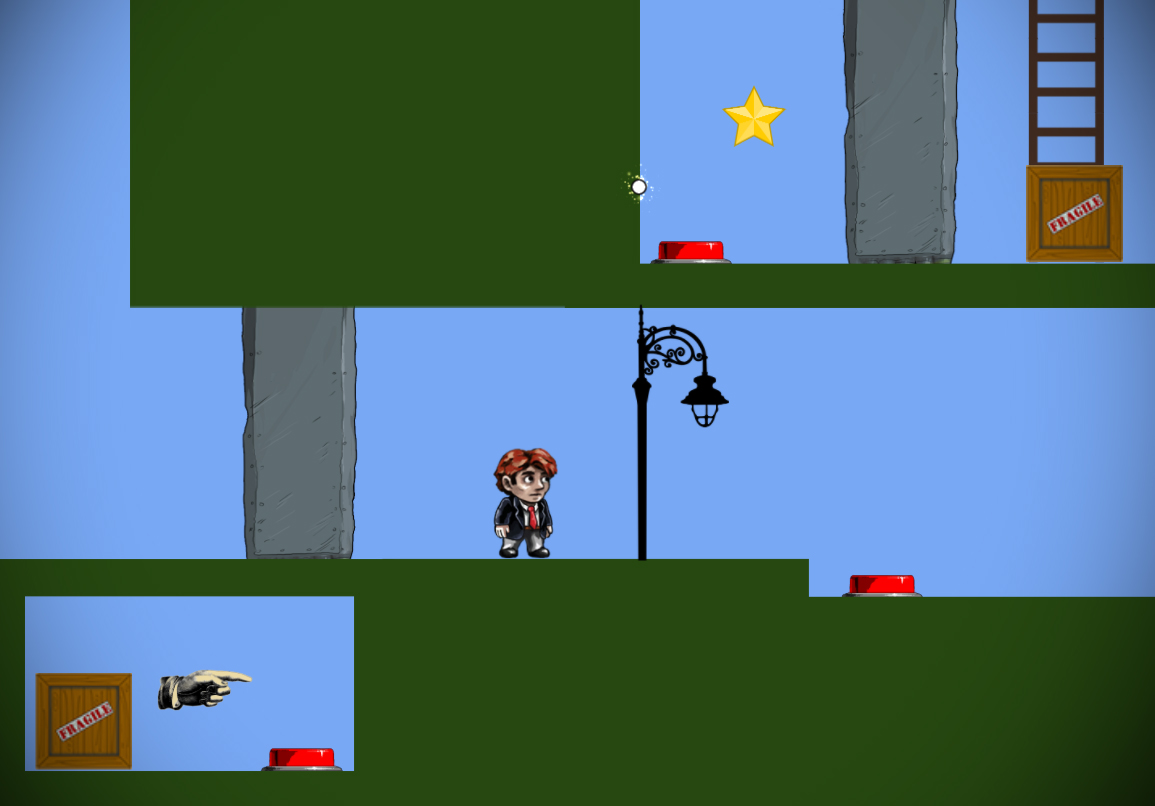
\includegraphics[width= 0.5\columnwidth]{images/gameDesign/30_grafica.jpg}
%	\caption{Esempio di elementi creati dal team grafico: cassa, bottoni, porta.}
%	\label{fig:ambientazione_team_grafico}
%\end{figure} 

\subsection{Personaggio principale}
\label{sec:main_character}

In Figura~\ref{fig:ambientazione_personaggio_01} vengono riportati alcuni schizzi sviluppati dalla componente del reparto grafico che si è occupato di \textit{Character Design}.

\begin{figure}%[h]
	\centering
	\includegraphics[width= \columnwidth]{images/gameDesign/31_personaggio_02.jpg}
	\caption{Schizzi del personaggio realizzati dal reparto grafico.}
	\label{fig:ambientazione_personaggio_01}
\end{figure} 

Come si può notare, le prime idee sviluppate prevedevano il controllo di un ragazzino, con una caratterizzazione che poteva farlo apparire interessato all’ambito culturale e quindi museale, da notare in particolar modo gli occhiali e la borsa a tracolla da studente. Parallelamente aveva però anche un aspetto molto giovanile e ribelle, sicuramente più attraente per un pubblico giovane. A tal riguardo, sono da sottolineare le scarpe, la camicia fuori dai pantaloni e la maglietta che esce dalla camicia.
Era dipinto con una silouette molto riconoscibile e quindi in possesso di una importante caratterizzazione.

Un personaggio del genere però, non sarebbe risultato molto attinente con le finalità di gioco. Il prodotto prevedeva che il personaggio fosse una trasposizione distorta del giocatore all’interno dell’ambientazione, così da permettere una maggiore immedesimazione. Caratterizzare quindi eccessivamente il personaggio avrebbe rischiato di sortire l’effetto contrario, e quindi allontanare e far percepire più distante il giocatore dal mondo di gioco.

Il passo successivo è stato quindi quello di studiare un nuovo personaggio, ma con caratteristiche più neutre, più impersonali e quindi più adatte allo scopo.
È stata scelta una colorazione scura uniforme, senza eccessivi dettagli, con i due occhi che spiccano decisamente rispetto al corpo. Inizialmente era stato anche ipotizzato di dotare il personaggio di un solo occhio, poi si è accantonata questa ipotesi, per distinguerlo maggiormente dai nemici. Il personaggio può comunque essere dotato di un vestito che possa renderlo più attraente e meno spoglio.

\begin{figure}%[h]
	\centering
	\includegraphics[width= \columnwidth]{images/gameDesign/32_personaggio_03.jpg}
	\caption{Schizzi più impersonali del personaggio realizzati dal reparto grafico.}
	\label{fig:ambientazione_personaggio_02}
\end{figure}

Come già spiegato nel capitolo relativo al design per le ambientazioni, per quanto riguarda gli asset sviluppati per il prototipo, ci siamo limitati a quegli elementi essenziali per la comprensibilità, l’usabilità e quindi verifica delle meccaniche di gioco.

Per quanto riguarda il personaggio quindi, abbiamo utilizzato i disegni forniti gratuitamente da David Hellman \cite{DavidHellmanSite} ed utilizzati per il videogioco Braid, da lui ideato e sviluppato.
Attualmente quindi, anche per quanto riguarda il personaggio principale, l’aspetto ottenuto, non è attinente con ciò che verrà mostrato nel prodotto finale.

\subsection{Nemici}
\label{sec:nemici}

Per quanto riguarda il design dei nemici si è scelto di caratterizzarli con un solo grande occhio ed un corpo buffo. Poiché le arti di cui trattiamo sono visive, i mostri hanno un occhio grande che possa riportare al concetto di visione. Nel concept iniziale, inoltre, il gioco assumeva una caratteristica molto più \textit{stealth}, con l’utilizzo costante dell’alternanza tra zone illuminate e zone d’ombra, così che l’occhio grande avesse ben potuto rendere l’idea del nemico cacciatore.

Nelle prime versioni del nemico, questo possedeva delle ciglia minacciose che avrebbero dovuto spingere il giocatore a fare attenzione nell’avvicinarsi ad esso (Figura~\ref{fig:ambientazione_nemico_01}).
Il corpo dovrebbe simulare l’idea di una lacrima scura che viene generata dall’occhio stesso.

\begin{figure}%[h]
	\centering
	\includegraphics[width= \columnwidth]{images/gameDesign/33_nemici.jpg}
	\caption{Schizzi del nemico realizzati dal reparto grafico.}
	\label{fig:ambientazione_nemico_01}
\end{figure}

L’idea preliminare di concept prevedeva che, mentre il personaggio fosse la trasposizione del giocatore nell’ambiente di gioco, i nemici fossero una rappresentazione astratta degli altri visitatori e di altri elementi del museo.
A partire quindi dall’idea base sono state sviluppate varie tipologie di nemici, osservabili in Figura~\ref{fig:ambientazione_nemico_02}, in ognuna con caratteristiche e comportamenti differenti a seconda della situazione:

\begin{itemize}
	\item \textbf{Minion}. Si tratta del nemico base. Molto goffo e quasi inoffensivo. È la trasposizione dei bambini che visitano il museo.
	\item \textbf{Predatore}. Ha denti più affilati, è più veloce e più intelligente. Trasposizione degli adulti, accompagnatori dei bambini.
	\item \textbf{Spesso}. È alto e con spalle larghe. Ha denti più grossi. È lento ed immune alle trappole. Trasposizione dei guardiani del museo.
	\item \textbf{Volante sentinell}. Un grande occhio alato. Non ha denti e non può ferire, ma avverte gli altri della presenza del personaggio principale. Trasposizione delle telecamere del museo.
	\item \textbf{Volante rapace}. Simile alla sentinella, ma con aspetto più minaccioso. Può ferire. Trasposizione dei piccioni della Mole Antonelliana di Torino.
\end{itemize}

\begin{figure}%[h]
	\centering
	\includegraphics[width= \columnwidth]{images/gameDesign/34_nemici.jpg}
	\caption{Schizzi delle varie tipologie di nemici.}
	\label{fig:ambientazione_nemico_02}
\end{figure}

Una volta delineate le meccaniche principali di gioco e le possibili ambientazioni, è stata quindi analizzata ogni tipologia di nemico, così da studiarne le caratteristiche ed estrapolarne ogni possibile meccanica interessante ai fini del gameplay.

È importante che ogni tipologia di nemico abbia caratteristiche uniche e non sovrapponibili, così da giustificarne l’esistenza e assicurare che il giocatore capisca il modo di approcciare ogni minaccia nel modo appropriato. Risulta fondamentale anche caratterizzarli a livello grafico, così che ogni azione sia giustificata e il comportamento possa essere prevedibile ancora prima che entrino in azione.

In seguito alla fase di design delle principali meccaniche, e dopo aver considerato gli obiettivi primari dello sviluppo del prototipo, abbiamo deciso di utilizzare due tipologie di nemici, visibili in Figura~\ref{fig:ambientazione_nemico_03}:

\begin{itemize}
	\item \textbf{Dumb}. È un personaggio goffo caratterizzato dall’aver l’occhio chiuso. Avanza fino ad incontrare un ostacolo e quindi torna indietro in un moto continuo. Uccide il personaggio principale al contatto. Può essere ucciso con un salto in testa o nel momento in cui raggiunge elementi danneggianti, come le punte infilzanti. Il salto in testa fornisce al personaggio una spinta verso l’alto.
	\item \textbf{Guard}. Graficamente risulta simile al dumb, se non fosse per un aspetto meno goffo e per l’avere l’occhio aperto. L’occhio suggerisce che controlli una porzione di scenario. Può trovarsi fermo in una posizione o proseguire con un moto simile a quello del dumb. Nel momento in cui vede il player di fronte a lui, entro un determinato raggio, inizia un’animazione di carica. Quando il personaggio esce dal suo campo visivo, risulta spaesato per qualche istante, poi torna alla precedente situazione. Il personaggio viene istantaneamente ucciso al contatto. Può essere stordito da un salto in testa del personaggio. Non viene ucciso se non andando a contatto di un elemento danneggiante, come le punte. Il salto in testa fornisce al personaggio una spinta verso l’alto.
\end{itemize}

\begin{figure}%[h]
	\centering
	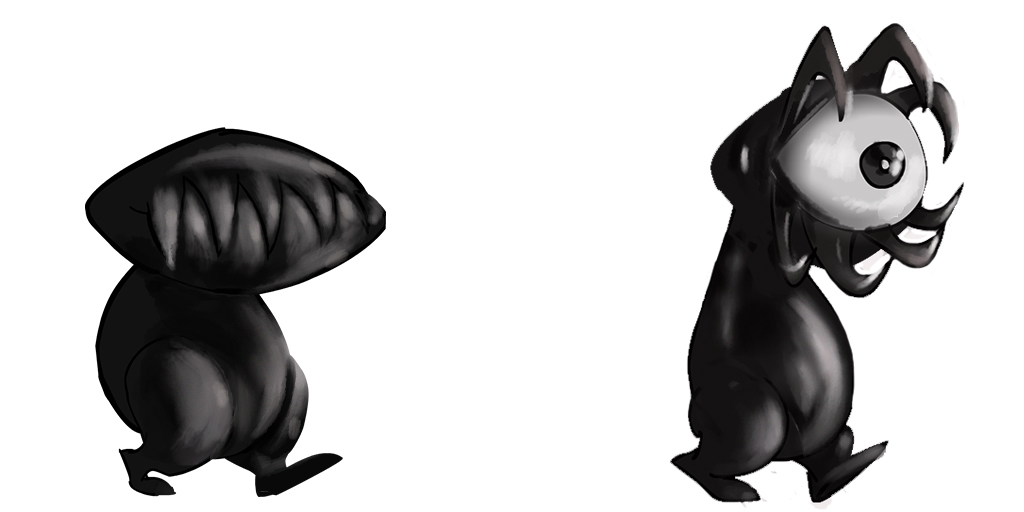
\includegraphics[width= 0.8\columnwidth]{images/gameDesign/35_nemici.jpg}
	\caption{Tipologie di nemici utilizzate nel prototipo.}
	\label{fig:ambientazione_nemico_03}
\end{figure}

Il \textit{dumb} è il primo nemico che si incontra, il suo comportamento è facile e prevedibile, viene utilizzato per permettere al giocatore di familiarizzare in maniera intuitiva con i nemici. Viene sfruttato soprattutto per premere pulsanti posti in luoghi non favorevoli al player o per raggiungere luoghi elevati grazie alla possibilità di saltargli in testa. Può essere guidato in diverse sezioni di gioco, ad esempio, cercando di sostituire un eventuale caduta con una proiezione di piattaforma (riferimento) o eliminando un ostacolo, ad esempio aprendo una porta.

Il \textit{guard} è un nemico più difficile da affrontare, in quanto reagisce direttamente alla presenza del nemico. Il moto di carica è più veloce di quello della semplice camminata, oltre che del player stesso, che è perciò costretto a fuggire o saltarlo con repentinità. La differenza principale di gameplay rispetto al \textit{dumb} consiste nel fatto che possa essere “guidato” facilmente in differenti sezioni di gioco, comportamento dovuto alla natura stessa del nemico che tende ad inseguire il personaggio.

\section{Audio e Suoni}
\label{sec:audio}

Per quanto riguarda l’audio presente del gioco, non siamo stati accompagnati da un reparto di esperti. Abbiamo quindi effettuato un design approfondito anche da questo punto di vista. 

Ogni elemento sonoro inserito è stato trovato online, dopo attente ricerche relative alle tematiche ed alle tipologie di suoni necessari. Chiaramente ogni elemento adoperato, è caratterizzato da una licenza gratuita, quindi liberamente utilizzabile per gli scopi del nostro progetto.

Per quanto riguarda la musica presente nei livelli, abbiamo ritenuto opportuno inserire, nell’\textit{hub centrale}, un tema che avesse generato sensazioni di sospensione e mistero. Il campione audio inserito è tale per cui la prima sezione risulti differente dalla seconda, caratterizzata invece da toni che generano sorpresa di fronte ai nuovi elementi che vengono mostrati a schermo e scoperti dal giocatore per la prima volta.
Nelle successive visite all’\textit{hub}, che avvengono nella transizione tra i livelli, la musica mantiene comunque una caratterizzazione misteriosa pur adattandosi alle nuove tematiche ascoltate nei livelli.

Questi sono caratterizzati da musiche decisamente più allegre. Il primo livello in particolare possiede un tema musicale molto frenetico ed agitato, che spinge il giocatore ad affrontare le prime sezioni \textit{platform} con spensieratezza, senza porre l’attenzione su elementi troppo impegnativi dal punto di vista della logica di gioco.
Con l’evolversi dei livelli, le musiche diventano decisamente più adatte alle meccaniche \textit{puzzle}, restano comunque luminose ed allegre, ma decisamente meno frenetiche di quella ascoltata nel primo livello. Tali temi tendono a rilassare il giocatore, pur mantenendo alta la sua attenzione durante le sezioni che richiedono maggiori abilità di ragionamento.

\section{Level Design}
\label{sec:level_design}

Per \textit{Level Design} si intende la creazione dell’ambiente di gioco a partire dalle meccaniche che si è deciso di includere. È un elemento di fondamentale importanza nella creazione di un prodotto videoludico. Senza un buon \textit{Level Design} l’esperienza può risultare noiosa e poco stimolante o eccessivamente frustrante, anche in presenza di ottime meccaniche di gioco.

\subsection{Principi di Level Design}
\label{sec:principi_level_design}

Nell’affrontare il design dei livelli sviluppati, abbiamo cercato di seguire dei passi che ci avessero permesso di ottenere i risultati prefissati, in modo ordinato.
La prima fase è quella di cercare di elencare ogni elemento che deve essere presente nel livello. Con “elemento” non si intendono solo gli oggetti che popolano lo scenario, ma anche quello che il giocatore deve riuscire ad imparare, a padroneggiare e le sfide di fronte a cui si deve porre. A titolo di esempio vengono riportati alcuni obiettivi che ci siamo posti per il primo livello:

\begin{itemize}
	\item Il giocatore deve imparare ad usare i tasti direzionali per muoversi.
	\item Deve imparare ad usare il salto.
	\item Deve padroneggiare la meccanica del salto.
	\item Deve capire che, attraverso l’utilizzo del puntatore, può osservare altre sezioni di gioco.
	\item Deve capire e dare per scontate le differenze tra le varie tipologie di terreno.
\end{itemize}

Una volta chiariti quali devono essere gli obiettivi, si inizia a disegnare su carta alcune sezioni che permettono di raggiungere lo scopo prefissato. Ogni sezione viene quindi analizzata attentamente per capire eventuali criticità, se sia necessario farla precedere da una sezione più facile con lo stesso scopo, se possa risultare troppo difficile per il livello scelto.

Dopo aver creato un buon numero di porzioni di livello si prova ad assemblarlo ed analizzarlo nel suo complesso per capire se ci sia necessità di inserire nuove sezioni o eliminarne di esistenti.
È in questo punto che risulta fondamentale il discorso già intrapreso in altri capitoli riguardo il cercare di mantenere l’utente nella situazione di \textit{flow} (Figura~\ref{fig:level_design_flow}). È infatti in questi momenti, in cui il giocatore non è annoiato o frustrato, che si possono ottenere, come risultati:

\begin{itemize}
	\item Estrema attenzione sull’obiettivo.
	\item Senso di controllo dell’azione.
	\item Sinergia tra azione e consapevolezza.
	\item Immedesimazione.
	\item Distorsione dell’esperienza del tempo.
	\item La ricerca dell’obiettivo che spinge a continuare.
\end{itemize}

\begin{figure}%[h]
	\centering
	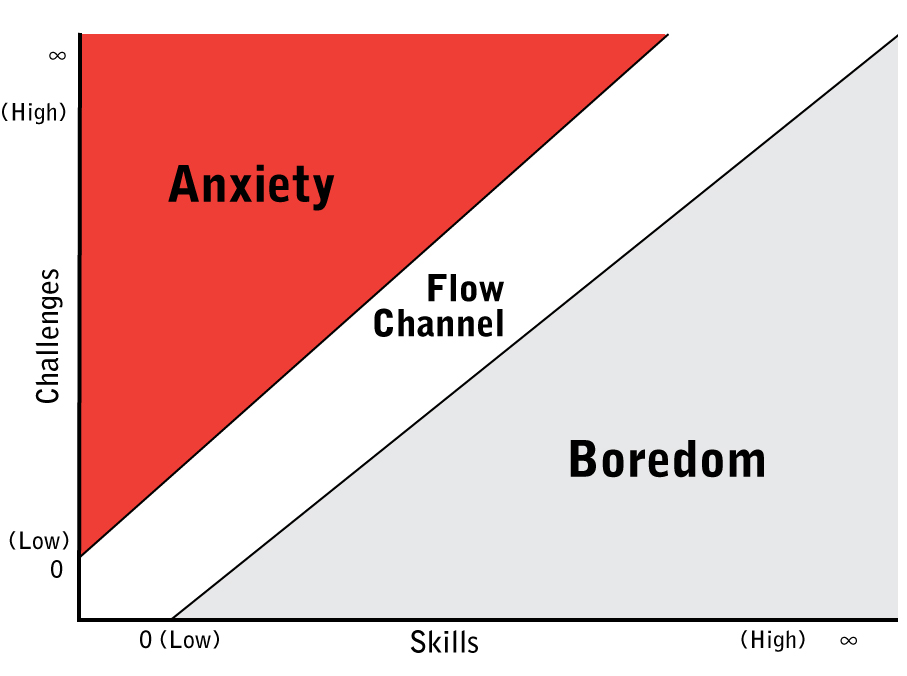
\includegraphics[width= 0.8\columnwidth]{images/gameDesign/36_flow.jpg}
	\caption{Rappresentazione grafica della situazione di Flow.}
	\label{fig:level_design_flow}
\end{figure}

Per far sì che il giocatore mantenga queste condizioni, è necessario che il livello accompagni l’utente lungo una curva di apprendimento che gli permetta di comprendere con facilità le meccaniche di gioco, di aumentare progressivamente il livello di difficoltà e permettere quindi un padroneggiamento delle meccaniche che generi soddisfazione e gratificazione.
È quindi necessario un attento studio degli elementi di gioco e degli equilibri che si devono venire a creare lungo la progressione del livello.
Una volta che si ha l’idea della struttura generale del livello, questo viene testato a fondo e modificato di conseguenza, in modo da perfezionare ogni dettaglio dell’esperienza di gioco, assicurandosi che gli obiettivi, che si erano descritti nella fase iniziale del \textit{Level Design}, siano stati raggiunti.
I passi che abbiamo seguito, e precedentemente descritto, sono in parte ispirati dall’articolo di Diorgo Jonkers, “How to design levels for a platformer” \cite{DiorgoJonkersArticle}.

Anche il libro The Art Of Game Design \cite{artOfGameDesign}, di Jesse Schell, fornisce alcuni interessanti spunti a riguardo, che ci hanno aiutato nella creazione delle varie sezioni di gioco.

La prima idea che emerge dall’analisi del capitolo “Game Mechanics Support Puzzles” è che i puzzles sono ovunque in un videogioco, spesso sono visibili e mostrati come tali, altre volte sono insiti nel gameplay, così da sembrare nascosti. Jesse Schell definisce puzzle ogni elemento di gioco che faccia fermare e pensare. Anche i giochi puramente action possiedono un gran numero di componenti puzzle, basti pensare ad una possibile battaglia con un boss di gioco. Il riuscire a capire il suo punto debole e come sfruttarlo a proprio vantaggio è un elemento puzzle. In un gioco di corse in cui si cerca di capire come superare l’avversario e si decide di sfruttarne la scia per ottenere una maggiore velocità, si sta risolvendo un puzzle. Ogni sezione di gioco che richieda l’utilizzo di una meccanica, in maniera non scontata, ha una componente puzzle.

Con l’evolversi dei videogiochi c’è stato un graduale passaggio dal puzzle esplicito a quello implicito, ma è esclusivamente dovuto al cambiamento di gusti dei giocatori ed alla maturazione delle abilità dei game designers.
L’autore ha definito dei principi, che abbiamo ritenuto fondamentali nello sviluppare ed architettare in maniera armoniosa tutti i livelli di gioco:

\begin{itemize}
	\item \textbf{Rendere l’obiettivo facile da capire.} Per fare in modo che i giocatori siano interessati, devono sapere cosa ci si aspetti che facciano.
	\item \textbf{Deve essere facile iniziare.} Una volta che il giocatore capisce l’obiettivo del puzzle, inizia a risolverlo. E con alcuni puzzle, è abbastanza chiaro come iniziare, sebbene non sia ovvio come risolverlo.
	\item \textbf{Dare un senso di progressione.} Ai giocatori piace la sensazione di fare progressi nel risolvere una situazione, dà loro speranza di stare arrivando alla risposta.
	\item \textbf{Dare un senso di risolvibilità.} Se il giocatore inizia a dubitare del fatto che un puzzle sia risolvibile, può diventare preoccupato del fatto di star perdendo tempo. Un modo per assicurarsi che ciò non avvenga è appunto mostrare dei progressi.
	\item \textbf{Aumentare gradualmente la difficoltà.} Abbiamo analizzato più volte questo punto. È un discorso che va molto al di là del singolo puzzle. In questo caso si intende la crescente difficoltà nel proporre al giocatore puzzle simili ma con soluzioni sempre più difficili, che lo invitino a superare i limiti raggiunti precedentemente.
	\item \textbf{Parallelizzare fa riposare il giocatore.} I puzzle, come già detto, fanno pensare a ragionare. C’è perciò il rischio concreto che un giocatore, incapace di fare progressi, abbandoni il gioco. Un buon modo per evitare questo comportamento è fornire contemporaneamente differenti puzzle, così che l’utente possa dedicarsi ad uno di questi e, nel caso dovesse fermarsi troppo a lungo, potersi dedicare ad un altro.
	\item \textbf{Un struttura a piramide estende l’interesse.} Significa che un insieme di piccoli puzzle, ognuno dei quali fornisce un piccolo indizio riguardo un puzzle più grande, aumentano l’interesse del giocatore. In questo modo è facile fornire dei piccoli obiettivi, raggiungibili più facilmente, che concorrono al raggiungimento di un obiettivo maggiore.
	\item \textbf{Gli aiuti estendono l’interesse.} Quando un giocatore sta per abbandonare un puzzle perché troppo difficile, fornirgli un aiuto può rinnovare la sua speranza e curiosità.
	\item \textbf{Dare la risposta.} Spesso basta far ragionare il giocatore e dare una risposta differente al puzzle. L’utente trova soddisfacente il momento in cui la risposta gli viene rivelata, anche se lui era arrivato ad una diversa conclusione. È lo stesso ragionamento che viene fatto per i libri, il lettore può immaginare un finale, ma è l’autore che fornisce la risposta e può essere completamente diversa da quella che si aspettava il lettore. Questo mezzo, se usato attentamente, può dare molta soddisfazione all’utente, portandolo ad incuriosirsi attraverso la sorpresa.
	\item \textbf{I “cambiamenti percettivi” sono un’arma a doppio taglio.} Per cambiamenti percettivi si intendono quei momenti in cui, osservando un determinato puzzle, si riesce a scoprire improvvisamente la soluzione, magari semplicemente cambiando prospettiva o attraverso un’idea inaspettata. Questo tipo di puzzle rischiano di portare a frustrazione il giocatore, in quanto si ottiene una grande soddisfazione nel caso si riesca a risolverlo, ma c’è un grande rischio che questo non avvenga, se, appunto, non si riesce ad avere l’idea giusta.
\end{itemize}

Come si vedrà nell’analisi dei livelli (riferimento) i concetti appena espressi hanno fornito una perfetta base per la creazione e lo sviluppo dei livelli di gioco.

\subsection{Scelte relative alla struttura dei livelli}
\label{sec:struttura_livelli}

Nelle prime fasi di Design si è deciso di strutturare l’esperienza di gioco in due fasi ben distinte. All’avvio della partita il giocatore si sarebbe trovato all’interno del museo. L’ambientazione sarebbe stata interamente in 3D, con la possibilità di controllare in prima persona il proprio personaggio. La visita al museo sarebbe dovuta proseguire in maniera lineare lungo un percorso standard. Sarebbero state presenti quindi teche con oggettistica e relative descrizioni.
All’interno dell’ambiente però, alcuni elementi avrebbero permesso al giocatore di infrangere delle regole e perciò uscire dalla visita standard, come una porta con scritto “Staff Only” (Figura~\ref{fig:level_design_staffonly}) o una teca con cui poter interagire per aprirla.

\begin{figure}%[h]
	\centering
	\includegraphics[width= 0.8\columnwidth]{images/gameDesign/37_museo3d.jpg}
	\caption{Rappresentazione tridimensionale del museo ipotizzata nelle prime sessioni di Design.}
	\label{fig:level_design_staffonly}
\end{figure}

Nel momento in cui il player avesse commesso quindi un’azione non prevista dalle regole dal museo, sarebbe entrato in un mondo parallelo, interamente bidimensionale, in cui sarebbero stati presenti la sua trasposizione e quella di tutti gli altri visitatori del museo.
L’ambientazione avrebbe dovuto rispecchiare gli spettacoli dell’epoca del pre-cinema, ispirandosi quindi, sia per meccaniche che per rappresentazione, all’oggettistica di riferimento.
I capitoli (riferimenti) affrontano in maniera approfondita l’analisi del design di ambientazioni e dei personaggi.

Dopo un’attenta analisi, si è preferito eliminare la prima sezione di gioco in prima persona, perché il passaggio alla seconda non sarebbe stato così immediato, oltre che rischioso da un punto di vista del messaggio comportamentale che avrebbe potuto trasmettere.

Si è quindi deciso di fare in modo che l’esperienza del giocatore non fosse direttamente collegata all’idea di museo, ma che ne richiamasse alcuni aspetti in maniera indiretta.
L’avventura avrebbe quindi assunto una caratterizzazione differente, con connotazioni pesantemente esperienziali. Si è pensato di abbandonare l’idea di sviluppare una ricca componente di storyline, ma far sì che l’esperienza vissuta dal giocatore fosse data dall’immersività nel mondo di gioco e dalle sensazioni che questo gli avesse potuto trasmettere.
Per questo tipo di approccio ci siamo in parte ispirati a videogiochi come LIMBO (riferimento), in cui si controlla un ragazzino, di cui si intuisce solo la sagoma. Ci si trova in un mondo, che ha l’aspetto di una foresta, ricco di pericoli, che metteranno a rischio l’incolumità del personaggio. Non è chiaro il perché il ragazzo si trovi in una tale situazione, ma è evidente che deve cercare di uscirne. L’esperienza di gioco è data appunto dalle sensazioni provate dal giocatore, garantite da un’ambientazione ricca di fascino e da meccaniche efficaci.


\section{Serious Game}
\label{sec:design_serious}

\section{Interfaccia}
\label{sec:design_interfaccia}
\chapter{Game Development}
\label{chap:game_development}

\section{Fasi dello sviluppo}

I lavori sul progetto ``The Magic Lantern'' sono iniziati a cavallo di Gennaio e Febbraio, dove i primi meeting con l'azienda sono serviti per spiegare i retroscena del progetto e il documento di game design iniziale.
Al secondo meeting è stata definitiva una timeline per l'intero lavoro, in buona parte rispettata. 

La timeline ha previsto una divisione del lavoro in due macro sezioni, dove in ognuna delle quali sono stati portati a termine vari sotto-fasi ed obiettivi:

\begin{itemize}

\item Pre Production: periodo stimato (Febbraio-Marzo)

\begin{itemize}
\item High Concept revision: all'inizio è servito rivedere il concept iniziale, recepire i feedback ricevuti dalla commissione Europea (per la quale il progetto si era precedentemente iscritto) e quindi riformulare, tramite varie sessioni di brainstorming, un nuovo concept.
\item Pitch: rielaborato il concept, si è spiegato tutto in un breve pitch, per definire bene i nuovi intenti di design.
\item Concept art revision: oltre al concept di gameplay si è fatto un concept anche a livello artistico.
\item Game Design Document updating: una volta approvato il pitch e le varie revisioni, l'obiettivo è stato quello di riscrivere il documento di game design.
\item Prototyping: definito il documento di design, si è creato un prototipo che confermi in prima battuta le scelte di design prese. Questi ultimi 2 step sono stati ripetuti più volte.
\end{itemize}

\item Production: periodo stimato (Aprile-Luglio)

\begin{itemize}
\item Game Design: una volta scelto il Game Design definitivo dalla fase precedente, questo è stato rivisto e ulteriormente raffinato.
\item Development: a questo punto, lo sviluppo vero e proprio della demo definitiva è partito.
\item Level Design: una grossa parte della production è stata dedicata al level design, in quanto, una volta creato un gameplay di base, è servito studiare come farlo fruire al giocatore.
\item Art production: a questo punto è stato necessario il supporto dal reparto grafico al fine di ``colorare'' e ``riempire'' il mondo di gioco. In genere gli artisti forniscono concept al resto del team al fine di fornire anche nuove idee per livelli e ambientazioni varie. In questo caso specifico, il reparto artistico ha fornito gli asset indispensabile per rendere il gioco chiaro e minimamente godibile.
\item Audio production: per ogni sezione di gioco è stato inserito il relativo audio, al fine di trasmettere le sensazioni volute al player.
\item First Playable: dopo aver tenuto conto di tutti i focus precedenti, si è passati alla creazione della prima versione giocabile della demo.
\item Testing alpha version: finalizzata la demo giocabile, questa va testata tramite il pubblico target, quindi vanno analizzati i risultati e i feedback raccolti.
\end{itemize}

\end{itemize}

La fase di Pre-Production è stata, in buona parte, rispettata. La fase di Production, invece, è stata ritardata di qualche settimana per via delle vacanze Pasquali e altre rielaborazioni varie che hanno riguardato gli ultimi due focus del pre-production (Game Design Document e Prototyping), in quanto è stato necessario provare più volte versioni dei design pensati (come è solito succedere per ogni videogame che attraversa questa fase). Qui sono state fatte varie prove di gameplay, tentando varie combinazioni di comandi per l'uso dello strumento centrale del gioco, la Lanterna Magica. Come già detto nel capitolo di Game Design (\ref{chap:game_design}), si è inoltre scelto di concentrare il gioco soprattutto sulle meccaniche intorno alla Lanterna, piuttosto che dare un uguale peso ad altre tecnologie del pre-cinema, se così non fosse stato, si sarebbero create troppe combinazioni e la complessità del gioco si sarebbe elevata troppo, considerati anche il tempo e i mezzi a disposizione. Si è scelto quindi di utilizzare le altre tecnologie in altri modi, come per esempio mini livelli o comunque sezioni limitate di gioco. In generale, questa fase ha visto un largo studio dello stato dell'arte dei giochi di interesse per il nostro studio, giochi sia di tipo Serious Game sia di tipo platform e puzzle. Si è quindi provato a prendere spunto dai pattern più famosi al fine di rendere il gioco il più comprensibile possibile.

La fase di Production, iniziata a fine Aprile, ha visto una fetta enorme di tempo dedicata al level design. Non è stato facile definire un livello di difficoltà per il pubblico target, ma in generale per il giocatore. In questa fase ci si è scontrati con dei veri problemi di design, e si è cercato di capire come una meccanica andrebbe fornita al player. Per fare ciò, ci si è ispirati in parte anche ai giochi esposti nella sezione dello stato dell'arte (\ref{chap:stato_dell_arte}). Dopo una lunga fase, durante la quale sono stati usati dei placeholder, è arrivato il supporto grafico per rendere il gioco più chiaro e adatto per un generico pubblico, questo supporto è arrivato a Giugno (nonostante fosse stato preventivato verso Aprile-Maggio). A causa di vari ritardi, come quello del supporto grafico, la continua re-implementazione dei livelli finali e la scelta delle modalità di fruizione dei contenuti Serious, la fase di Production (della demo) non si è potuta concludere a Luglio, come stabilito. Questo perché si è riusciti a portare a termine solo il primo round di testing, mentre era necessario farne almeno un secondo per apportare le modifiche necessarie in base ai feedback ricevuti durante il primo round, e quindi capire valutare l'efficacia dei cambiamenti applicati. Ovviamente, prima dei test esterni, sono state svolte varie sedute di testing interno all'azienda, per capire se il prodotto fosse pronto per un pubblico esterno.


\section{Strumenti}

The Magic Lantern è stato implementato tramite il game engine Unity3d versione 5.1.1.f1 (\url{https://unity3d.com}) usando prevalentemente il linguaggio di programmazione C\#. Unity3d è un game engine che fornisce un editor molto user-friendly, col quale si può familiarizzare anche in poche ore (presupponendo una minima base sulla computer graphic e l'informatica in generale). Esistono moltissimi tutorial sul web riguardo Unity3d, e la community è molto attiva, ciò semplifica ancor di più l'apprendimento dello strumento.

Come sistema di versioning è stato utilizzato Git (\cite{github}), tramite il programma SourceTree che fornisce una interfaccia grafica molto facile da utilizzare.

E' stato utilizzato inoltre, come strumento di team management e comunicazione interna, il programma Asana (\cite{asana}). Questo è uno strumento molto utile per assegnare task e fissare scadenze, cose essenziali per lavorare in team.


\section{Logica implementativa di gameplay}

\section{Controller del player}
\label{sec:player_movements}

Il videogioco si basa su classiche meccaniche \textit{platform}, il personaggio deve perciò essere capace di correre, saltare, salire scale. La classe \textit{playerMovements} si occupa appunto di gestire questi comportamenti.
Il player è gestito da una macchina a stati, mostrata in Figura~\ref{fig:development_player_stati}, che ne descrive lo stato attuale ed eventuali transizioni.

\begin{figure}%[h]
	\centering
	\includegraphics[width= 0.9\columnwidth]{images/development/player.jpg}
	\caption{Diagramma con gli stati del player.}
	\label{fig:development_player_stati}
\end{figure}

La classe, in primo luogo, si occupa di controllare se il player stia toccando terra o meno. Nel primo caso, il giocatore può utilizzare i tasti direzionali per cambiare il suo stato da \textit{idle} a \textit{running}. Inoltre, se l’attuale direzione risulta opposta a quella di movimento, il cambio di stato è preceduto da un’inversione di scala del personaggio.
Oltre alle situazioni in cui questo tocchi terra, il player può trovarsi nello stato di \textit{air}. In questa situazione i tasti direzionali possono essere utilizzati per controllare la caduta, in maniera limitata rispetto a quanto avviene a terra.
Lo stato di \textit{air} può essere raggiunto in due modi:

\begin{itemize}
	\item Spiccando un salto mentre è verificata la condizione di ground. In questo caso viene applicata una forza positiva lungo l’asse y.	
	\item Lasciandosi cadere da una sporgenza.
\end{itemize}

Raggiungendo lo stato \textit{air} il player mantiene la sua velocità lungo l’asse x, che può essere in parte limitata tramite i tasti direzionali, ma è soggetto ad una forza di gravità che lo spinge verso il basso.
La gravità, secondo canoni tipici dei giochi platform, è triplicata rispetto a quella standard, l’accelerazione di caduta risulta perciò molto enfatizzata. La velocità è comunque limitata da un valore massimo.
Oltre agli stati citati, esiste quello di \textit{onLadder}, questa particolare situazione descrive il personaggio mentre questo si trova ad utilizzare un scala. Il giocatore può decidere di scendere o salire attraverso i tasti direzionali. Lo stato può essere raggiunto sia quando il player è a terra, che quando si trova nella situazione \textit{air}, semplicemente premendo un tasto direzionale, lungo l’asse verticale, nei pressi di una scala.
Per lasciare lo stato di \textit{onLadder} esistono più modi:

\begin{itemize}
	\item Premendo un tasto direzionale lungo l’asse orizzontale. Viene impressa una piccola forza laterale al player, e questo passa allo stato di \textit{air}.	
	\item Raggiungendo la base della scala, se nella parte sottostante è presente un terreno, il personaggio la lascia, entrando nello stato ground, \textit{idle}.
	\item Raggiungendo la base della scala, se nella parte sottostante non è presente un terreno, il personaggio la lascia, entrando nello stato \textit{air}.
\end{itemize}

La classe \textit{playerMovements} è anche utilizzata come interfaccia dalle classi dell’\textit{AI} per richiamare metodi di movimento dei personaggi.

\section{Lanterna Magica e vetrini}

L’utilizzo della Lanterna Magica è la meccanica di gioco principale, questa permette di proiettare oggetti nell’ambientazione e modificare lo scenario di gioco.
Le classi \textit{MagicLantern} e \textit{MagicLanternGraphic} ne gestiscono interamente il comportamento.
\textit{MagicLantern}, classe derivata di \textit{Tool}, si occupa dello stato attuale della Lanterna e dei vari cambiamenti di stato in base all’input dell’utente.

\begin{figure}%[h]
	\centering
	\includegraphics[width= 0.9\columnwidth]{images/development/lanterna.jpg}
	\caption{Diagramma con gli stati della Lanterna Magica.}
	\label{fig:development_lanterna_stati}
\end{figure}

Come mostrato in Figura~\ref{fig:development_lanterna_stati}, la Lanterna si può trovare nei seguenti stati:

\begin{itemize}
	\item \textit{\textbf{NotUsed.}} Non è utilizzata dall’utente e risulta non visibile a schermo
	\item \textit{\textbf{InHand.}} Il personaggio sta usando la Lanterna, viene quindi mostrata a schermo, sovrapposta al player, ed il giocatore può usare il puntatore per mirare, prima di rilasciare e creare la proiezione.
	\item \textit{\textbf{Left.}} Il giocatore ha mirato e lasciato la Lanterna a terra. Questa sta perciò proiettando.
	\item \textit{\textbf{TurnedOff.}} La Lanterna è stata toccata da un nemico che l’ha spenta. Questo stato non è attualmente utilizzato nel prototipo sviluppato, in quanto si è negata la possibilità al nemico di spegnere la Lanterna.
	\item \textit{\textbf{Falling.}} La Lanterna sta cadendo.
\end{itemize}

All’inizio della partita, il giocatore non possiede ancora la Lanterna Magica, il \textit{gameObject} con la classe \textit{MagicLantern} è quindi disabilitato. Al primo raccoglimento della Lanterna, questa si trova nello stato \textit{NotUsed}. Il giocatore può quindi iniziare a mirare e passare allo stato \textit{InHand}. In questo stato la Lanterna è figlia del player, quindi lo segue durante i suoi movimenti.
Il giocatore può continuare a mirare, ad esclusione degli stati \textit{air} ed \textit{onLadder} del player (Capitolo \ref{sec:player_movements}).
Al momento del rilascio del tasto utilizzato per mirare, la Lanterna viene lasciata a terra, raggiunge perciò lo stato \textit{Left} e la proiezione viene resa tangibile ed interagibile. Se, al momento del rilascio, il player si trovava negli stati non adatti alla proiezione, precedentemente specificati, la Lanterna raggiunge lo stato \textit{NotUsed}.
Dallo stato \textit{Left}, la Lanterna può tornare direttamente a quello \textit{InHand} se l’utente preme il tasto per mirare, oppure a \textit{TurnedOff}, se è raggiunta da un nemico, o \textit{Falling} se il terreno sottostante scompare.
Dallo stato \textit{Falling}, la Lanterna raggiunge direttamente quello \textit{NotUsed} dopo un breve intervallo temporale.

La classe \textit{MagicLantern}, a seconda dello stato attuale, invoca particolari metodi della classe \textit{MagicLanternGraphic}, che si occupa invece di gestire la grafica dell’oggetto.
Il puntatore viene utilizzato per mirare, durante queste fasi, la sagoma della proiezione segue il puntatore, attraverso una funzione di \textit{smoothing} che rende i movimenti più piacevoli. La direzione del raggio viene quindi calcolata dinamicamente sulla base delle posizioni del player e della proiezione.
\textit{MagicLanternGraphic} si occupa quindi anche di spegnere ed accendere la lanterna, oltre che di cambiare la grafica del raggio, in modo da mostrare coerentemente gli stati \textit{InHand} e \textit{Left}.


\section{AI e spawner}

Poiché il gioco prevede l'interazione con dei nemici, è stato necessario sviluppare una logica di AI. Essendo il comportamento designato per i nemici non molto complesso, si è scelto di utilizzare una macchina a stati come logica di base, evoluta in un secondo momento in una macchina a stati gerarchica.

E' possibile vedere un Class Diagram rappresentante dell'implementazione usata:

\begin{figure}[h]
\centerline{\includegraphics[scale=0.45]{images/development/classdiagramAI.png}}
\caption{Class Diagram della AI usata.}
\label{fig:classdiagramAI}
\end{figure}

Il funzionamento di questa macchina a stati da la possibilità di gestire il comportamento di uno stato a diversi livelli di profondità, nonostante nell'implementazione finale sia stato usato un livello di profondità massimo pari a 2, si può potenzialmente andare ben oltre.
L'idea è che le azioni fatte dall'AI saranno presenti sempre nelle foglie della gerarchia, cioè in quegli stati che non avranno figli. Negli stati intermedi, oltre che nello stato foglia medesimo, si avrà la logica per il controllo di eventuali cambi di stato.
La scelta di questa logica permette una gestione ordinata dei passaggi di stato, oltre che un buon riuso del codice. Per esempio, lo stato intermedio \manclass{Patrol} può avere più stati figli sotto di sé, quali: \manclass{SuspiciousPatrol}; \manclass{WalkPatrol}; \manclass{StandPatrol}; \manclass{AreaPatrol} (nota bene, nel parlare di stati foglia, stati padre e stati figli, non si intendono concetti di ereditarietà tipica della programmazione ad oggetti). Questi ``stati foglia'', oltre che essere collegati fra loro da transizioni di stato (per esempio tutti sono collegati a \manclass{SuspiciousPatrol} e \manclass{WalkPatrol}, mentre gli altri due sono in genere esclusivi fra loro), sono tutti collegati anche ad altri stati. Quando tutti gli stati sotto lo stesso stato padre presentano la medesima transizione, allora di questa transizione è responsabile il padre, la logica di controllo è quindi definita nella classe del padre, infatti, come già detto, a controllare la necessità di transizione sono sia lo stato attivo sia gli stati gerarchici sopra quello stato. Per esempio, quando il player salta in testa ad un nemico mentre si trova in uno dei suoi stati \manclass{Patrol}, questo passerà in ogni caso allo stato \manclass{Stunned} che gestisce la morte o il temporaneo ``intontimento'' dei nemici.

Detto ciò, l'implementazione di un nemico prevede l'uso di una classe derivata da \manclass{AIAgent}, per esempio \manclass{AIGuard} e al suo interno andranno specificati gli stati padre e figlio da utilizzare (come \manclass{Patrol} e \manclass{WalkPatrol} etc). L'implementazione è basata sull'uso di delegati, invocati da \manclass{AIAgent}, in particolare sono invocati i delegati degli stati padre superiori, i quali, invocheranno in modo ricorsivo tutti i delegati fino a finire la gerarchia. 

I delegati, usati per ogni stato, sono:

\begin{itemize}

\item \manclass{Initialize}: invocato quando si entra nello stato dopo una transizione.
\item \manclass{Finalize}: invocato quando si esce dallo stato a causa di una transizione.
\item \manclass{Update}: invocato dallo stato attivo ogni frame, viene quindi invocato durante la funzione \manclass{Update} di \manclass{AIAgent}.
\item \manclass{StateTransition}: è un array di delegati che controllano se occorre effettuare una transizione di stato, vengono invocate durante la funzione \manclass{Update} di \manclass{AIAgent}, prima che venga invocato anche il delegato \manclass{Update}.
\item \manclass{TriggerEnter}: viene invocato quando viene invocata la funzione \manclass{OnTriggerEnter2D} di \manclass{AIAgent}.
\item \manclass{CollisionEnter}: viene invocato quando viene invocata la funzione \manclass{OnCollisionEnter2D} di \manclass{AIAgent}, invocata per esempio quando il nemico tocca il player o un muro.

\end{itemize}

L'implementazione scritta della macchina a stati non è ancora definitiva al 100\%, in quanto deve essere costruito uno schema che sia in grado di prevenire errori dall'errata impostazione della macchina, quindi occorre l'implementazione di metodi o di interfacce che agevolino questo compito.

Mentre il nemico ``Dumb'', non è in grado di fare delle azioni ``ragionate'', ma semplicemente cammina avanti e indietro, fin quando non trova la morte sul suo cammino (dovuta al player o all'ambiente), il secondo (la cui macchina a stati è mostrata in \myfig{\ref{fig:gerarchiaAIGuard}} ) invece presenta un minimo ragionamento, avendo degli stati che gli permettono di fare la guardia ad un posto o un area e riconoscere il player, quindi attaccarlo con una carica e ucciderlo al contatto (a meno che il contatto non avvenga sulla sua testa, in quel caso muore il Guard).

\begin{figure}[h]
\centerline{\includegraphics[scale=0.45]{images/development/gerarchiaAIGuard.png}}
\caption{Gerarchia macchina a stati del nemico ``Guard''.}
\label{fig:gerarchiaAIGuard}
\end{figure}

Infine, diciamo che correlato ai nemici, c'è lo script che gestisce la loro generazione, chiamato \manclass{spawner}. Questo genera da 1 ad ``n'' nemici, ad un ritmo di ``tot'' secondi (personalizzabile anche questo), avendo cura di controllare quanti nemici generati siano ancora in vita, così da non sforare il limite massimo scelto. Quando un nemico muore, se generato da uno spawner, richiama un metodo dell'istanza del relativo \manclass{spawner}, avvisando che è morto, quindi decrementando il contatore interno di nemici in vita.

\section{Menù, schede informative e contenuti sbloccabili}

Sia il menù di pausa che l'interfaccia utente delle schede informative, sono state implementate tramite l'uso della ``UI'' di Unity3d, un componente dell'editor Unity aggiunto nella versione 4.6. Gli script che regolano l'uso sono rispettivamente \manclass{MenuManager} e \manclass{InformativeManager}. Il primo gestisce il menù di pausa, mentre il secondo la navigazione dei contenuti Serious del gioco (oltre che metodi per analizzare quanto i contenuti siano stati letti, ma di questo parleremo nella sezione \ref{analisiFruizione}). 

Quando si entra in pausa, il timeScale passa a zero (una proprietà di Unity che regola lo scorrere del tempo) e si tiene traccia che non si è in gioco anche tramite una variabile statica della classe \manclass{PlayStatusTracker}, ``inPlay'', se questa è true, è attivo o il menù o l'interfaccia delle schede informative.
Il menù da la possibilità di ricominciare il livello, uscire dal gioco (e accedere alla prima scena con il menù principale) e accedere alle schede informative. 

La sezione di schede informative, come descritto nella sezione di design (\ref{chap:game_design}), è navigabile in modo da accedere a vari contenuti con le relative immagini. Lo sblocco di un contenuto, avviene tramite lo script \manclass{UnlockContent}, il quale comunica ad \manclass{InformativeManager} quale contenuto è stato sbloccato.

\section{UI in-game}

Le classi \textit{PlayingUI} e \textit{PlayingUILateral} si occupano di fornire dei metodi di accesso agli elementi che costituiscono l’interfaccia di gioco.

\textit{PlayingUI} si occupa dei 4 angoli dello schermo. Per ognuno di essi esiste la possibilità di specificare un’immagine o una serie di esse, da poter essere mostrate in verticale o orizzontale.
Le immagini possono quindi essere di tre dimensioni predefinite, così da fornire la possibilità di evidenziare determinati elementi, oltre che accompagnate dalla grafica di un bottone, di dimensioni standard, anche questo posizionabile in basso o lateralmente rispetto alla serie di immagini.
La classe fornisce chiaramente metodi per cambiare immagini, nasconderle, mostrarle ed accedere direttamente agli oggetti che costituiscono l’interfaccia.
Attualmente, nel prototipo sviluppato, viene utilizzata per mostrare in alto a destra il comando da premere per aprire le schede informative, come si può osservare in Figura~\ref{fig:interfaccia_ingame} e per mostrare al giocatore il vetrino attualmente utilizzabile dalla Lanterna Magica.

\textit{PlayingUILateral} invece, offre metodi simili a quelli di \textit{PlayingUI}, con la differenza data dal fatto che si occupa principalmente di gestire le sezioni laterali dell’interfaccia di gioco.
Permette quindi di creare due serie di immagini a destra ed a sinistra dello schermo, inserite in una barra che funge da contenitore. Questi insiemi di oggetti possono essere quindi mostrati e nascosti dinamicamente.
Attualmente viene utilizzata per mostrare all’utente gli oggetti e le stelle raccolte, rispettivamente nella parte destra e sinistra dello schermo, come mostrato in Figura~\ref{fig:rigiocabilita_UI_hub}.


\section{GeneralFinder e Utils}

Sono stati creati degli script per agevolare e rendere più efficiente le varie logiche di gioco. Per esempio, è stato creato uno script, chiamato \manclass{GeneralFinder} che raccoglie tutti i riferimenti più importanti della scena (come \manclass{PlayerMovements}, \manclass{InformativeManager} etc) e li immagazzina in variabili statiche, in modo che se un qualunque script debba in una qualunque parte del codice, accedere allo script del player, può farlo così: \manclass{GeneralFinder.PlayerMovements}, senza quindi dover cercare ogni volta il GameObject che lo contiene.

L'altro script creato ai fini di un risparmio di codice e resa efficiente del tutto, è \manclass{Utils} il quale implementa delle funzioni simili a quelle della libreria standard di Unity3d, ma dando funzionalità aggiuntive, utili sia per il nostro progetto sia per altri progetti generici.

\subsection{Oggetti interagibili}

La classe \textit{InteragibileObject} si occupa di fornire un’interfaccia standard per tutti gli oggetti dello scenario con cui è possibile interagire. È quindi utilizzata da leve, porte di fine ed inizio livello, oggetti collezionabili, personaggi non giocabili con cui dialogare. Dispone di metodi che mostrano a schermo il comando che il giocatore deve utilizzare per interagire con gli oggetti. Il comando si adatta dinamicamente all’uso o meno del controller.
I metodi di interazione e la grafica del comando da utilizzare vengono mostrati esclusivamente quando il giocatore si trova nei pressi dell’oggetto e scompaiono quando questo si allontana.
Al momento dell’interazione vengono invocati i metodi di oggetti specificati con variabili pubbliche tramite \textit{inspector}.

\subsection{Porte con bottoni}

L'utilizzo di porte che vengono aperte da bottoni avviene frequentemente nel gioco. Il comportamento più usato nel gioco prevede la pressione del bottone e il relativo innalzamento della porta corrispettiva, questa tornerà poi giù quando il bottone verrà rilasciato. Nonostante questo sia l'unico comportamento presente nella demo giocabile, sono state implementate delle varianti per l'apertura delle porte, una per esempio prevede che la porta rimanga alzata anche dopo il rilascio del bottone, oppure un'altra variante ancora prevede che la porta si apra (raggiungendo il suo picco di apertura) fin quando il bottone è premuto, quando invece nella configurazione di default basta toccare anche per un solo istante il bottone per fare aprire completamente la porta. Inoltre la logica prevede la possibilità di unire in serie più porte o meccanismi, sia in traslazione che in rotazione, al fine di risolvere degli enigmi presenti nei livelli di gioco. Sono stati previsti vari modi per premere un bottone, fra i quali, il passaggio del player, quello di un nemico o quello di un oggetto cassa.

\begin{figure}[h]
\centerline{\includegraphics[scale=0.35]{images/development/portaebottone.png}}
\caption{Focus su porta e bottone, dal gameplay di The Magic Lantern.}
\label{fig:portaebottone}
\end{figure}

%\subsection{Camera}

%\subsection{Altro...}

\section{Strumenti per il testing}

\subsection{Analisi di gameplay}
\label{sec:analisi_gamplay}

Durante lo sviluppo è risultato fondamentale studiare metodi efficaci per analizzare il gameplay dei giocatori e dei tester con strumenti oggettivi che ci avessero permesso di ricavare utili statistiche, ai fini di revisione del design e delle soluzioni applicate.
Abbiamo perciò sviluppato alcuni strumenti che ci avessero fornito informazioni riguardo:

\begin{itemize}
	\item Tempo trascorso in ogni porzione di livello.
	\item Game Over del personaggio.
	\item Equilibrio e organizzazione del Level Design.
	\item Difficoltà del gioco.	
\end{itemize}

Di seguito vengono quindi trattate alcune classi sviluppate appositamente per gli scopi appena esposti, con l’aggiunta di un sistema di replay della partita.

\paragraph{ZoneAnalyzer.}
\label{par:zone_analyzer}
È una classe che si occupa di salvare su file i dati relativi al tempo trascorso dal giocatore in ogni sezione di gioco. Il suo comportamento può essere quello di \textit{colelctor} o \textit{analyzer}. Ogni analyzer sfrutta uno o più collider di tipo \textit{trigger} che delimitano la porzione di gioco da analizzare. Quando il personaggio si trova all’interno della zona, viene incrementata una variabile che tiene conto del tempo trascorso. In ogni scena esiste un solo collector, che si occupa invece, al momento della chiusura del livello o del gioco, di raccogliere i dati di tutti gli analyzer e salvarli in un file .xml. Inoltre, ogni volta che il personaggio va in Game Over, lo script \textit{playerMovements} invia un messaggio che specifica il tag dell’oggetto che ha ucciso il player. In questo modo, si può tenere traccia, per ogni zona, del numero di morti generate da:

\begin{itemize}
	\item Nemici.
	\item Punte infilzanti.
	\item Porte.
\end{itemize}

\paragraph{HintAnalyzer.}
\label{par:hint_analyzer}
Si occupa di salvare su file .xml il numero di utilizzi di ogni aiuto usato nel gioco. Esistono alcuni trigger, in varie sezioni di gioco, che, nel caso il personaggio rimanga per troppo tempo al loro interno, fanno comparire un aiuto che permette al giocatore di non rimanere bloccato. Ogni volta che un aiuto viene attivato, la classe \textit{TutorialHInt}, che si occupa di gestirli, invia un messaggio all’HintAnalyzer, che riesce quindi a tener conto delle volte che il giocatore ha fatto uso di aiuti. Questa classe ci fa capire se il bilanciamento della curva di difficoltà è adeguato o meno.

\paragraph{SpikesAnalyzer.}
\label{par:spikes_analyzer}
Classe sviluppata inizialmente per calcolare il numero di morti dovute a punte infilzanti. In seguito all’ampliamento della classe \textit{ZoneAnalyzer}, è stata utilizzata soprattutto per verificare la difficoltà dei salti. Anche questa può avere il comportamento di \textit{analyzer} e \textit{collector}, i primi si occupano di contare il numero di volte in cui il player collide con dei trigger, il collector raccoglie quindi tutti i dati e li salva su .xml. Viene posto un analyzer nella porzione immediatamente sottostante ad un salto, così che, se si notano numeri troppo elevati, significa che il salto era troppo difficile e poco bilanciato.

\paragraph{Sistema di replay.}
\label{par:replay}
È stata appositamente creata la classe \textit{InputKeeper}, che funge da interfaccia per ogni input utilizzato dall’utente. La classe, se appositamente impostato, si occupa di salvare su file ogni variazione sugli input, accompagnandola dal tempo, in secondi, in cui è avvenuta. Con una diversa impostazione, la classe può fare in modo di utilizzare dei dati precedentemente salvati per simulare degli input dell’utente, invece caricati da file. In questo modo è possibile riosservare l’intera partita di un giocatore, e capirne eventuali criticità.

\subsection{Analisi della fruizione di contenuti Serious}
\label{analisiFruizione}

Per capire quanto i contenuti Serious vengano letti o visti dagli utenti, in vista del testing, sono stati usati gli script \manclass{InformativeManager} e \manclass{TestInformativeManager}. Il salvataggio dei dati avviene tramite un xml dove nel quale si serializza la classe \manclass{InfoSectionContainer}, la quale contiene informazioni riguardo i contenuti (\manclass{InformativeContent} e \manclass{SubContent}) e le relative sezioni (\manclass{InformativeSection}).

I dati salvati riguardano:

\begin{itemize}

\item I tempi, oltre che il numero di volte, impiegati per visualizzare una scheda informativa (cioè un contenuto), avendo pure il dettaglio per sotto-contenuto. Si è tenuto traccia pure del fatto che la scheda sia stata aperta o meno una volta sbloccata o se fosse stata vista in un secondo momento.
\item Poiché sono presenti dei quiz durante i livelli (riguardo i contenuti Serious), si è tenuto traccia del numero di tentativi sbagliati e se alla fine si è risposto in modo corretto.

\end{itemize}

\newpage
\chapter{Risultati e obiettivi, sviluppi futuri}
\label{chap:risultati}

%\appendix
% INCLUSIONE APPENDICI - - PERSONALIZZARE - TENERE COERENTE CON LISTA IN ALTO
%% !TEX root = ../thesis.tex
\chapter{An appendix}
\label{app:a}

appendix


%%%%%%%%%%%%%%%%%%%%%%%%%%%%%%%%%%%%%%%%%%%%%%%%%%%%%%%%%%%%%%%

% BIBLIOGRAFIA
\addcontentsline{toc}{chapter}{\refname}
\nocite{*}
\printbibliography

\end{document}